% Intended LaTeX compiler: pdflatex
\documentclass[12pt,a4paper,twoside]{ugathesis}
\usepackage[utf8]{inputenc}
\usepackage[T1]{fontenc}
\usepackage{graphicx}
\usepackage{grffile}
\usepackage{longtable}
\usepackage{wrapfig}
\usepackage{rotating}
\usepackage[normalem]{ulem}
\usepackage{amsmath}
\usepackage{textcomp}
\usepackage{amssymb}
\usepackage{capt-of}
\usepackage{hyperref}
\usepackage[citestyle=authoryear, bibstyle=authoryear, hyperref=true,backref=true,maxcitenames=2,url=true,backend=biber,natbib=true]{biblatex}
\addbibresource{biblio.bib}
\usepackage{amsthm, bm}
\usepackage[francais]{babel}
\usepackage[table]{xcolor}% http://ctan.org/pkg/xcolor
\usepackage{float}
\usepackage{tikz}
\usetikzlibrary{calc}
\usepackage{sectsty}
\usepackage{float}
\usepackage[figuresleft]{rotating}
\usepackage{epigraph}

%% théorèmes
\newtheorem{theorem}{Théoreme}
\newtheorem{corollaire}{Corollaire}
\newtheorem{proposition}{Proposition}
\renewcommand{\proofname}{Preuve}


%% defining colors
\definecolor{customDarkGreen}{RGB}{47,79,79}
\definecolor{customDarkGrey}{RGB}{25,25,25}
\definecolor{customGreen}{RGB}{41,124,120}
\definecolor{customGrey}{RGB}{105,105,105}
\definecolor{customSteelBlue}{RGB}{65,131,196}

%% coloring title
\chapterfont{\color{black}\huge}  % sets colour of chapters
\sectionfont{\color{customGreen}\LARGE}  % sets colour of sections
\subsectionfont{\color{customDarkGrey}}
\subsubsectionfont{\color{customGrey}}  % sets colour of sections

%% hyperlink
\hypersetup{unicode=true,
            colorlinks=true,
            linkcolor=black,
            citecolor=customSteelBlue,
            urlcolor=customSteelBlue,
            breaklinks=true}

%% table
\newcolumntype{x}[1]{>{\centering\arraybackslash\hspace{0pt}}p{#1}}

%% common 
\newcommand{\matr}[1]{\mathbf{#1}} %% \matr{}
\newcommand{\Y}{\matr{Y}} %% Output matrix
\newcommand{\Yrow}{n} %% Y row dim
\newcommand{\Ycol}{p} %% Y col dim
\newcommand{\Id}{\matr{Id}} %% \Id
\newcommand\norm[1]{\left\lVert#1\right\rVert} %% \norm
\newcommand{\pvalue}{$p$-value} %% \pvalue
\newcommand{\Var}{\mathrm{Var}} %% variance
\newcommand{\RR}{\mathbb{R}} %% real ensemble
\newcommand{\Normal}{\mathcal{N}} %% Normal distribution

%% name of method
\newcommand{\MethodCate}{CATE}

%% name of software
\newcommand{\RpackageCate}{{\tt cate}}


%% lattent factor model
\newcommand{\K}{K} %% number of latent factor
\newcommand{\U}{\matr{U}} %% factor score matrix/ records latent variables
\newcommand{\Ucol}{\K} %% U col dim
\newcommand{\Urow}{\Yrow} %% U row dim
\newcommand{\V}{\matr{V}} %% factor loading matrix
\newcommand{\Vcol}{\K} %% V col dim
\newcommand{\Vrow}{\Ycol} %% V row dim
\newcommand{\X}{\matr{X}} %% primary matrix / record primary variable
\newcommand{\Xcol}{d} %% X col dim
\newcommand{\Xrow}{\Yrow} %% X row dim
\newcommand{\B}{\matr{B}} %% primary effects matrix
\newcommand{\Bcol}{\Xcol} %% B col dim
\newcommand{\Brow}{\Ycol} %% B row dim
\newcommand{\E}{\matr{E}} %% residual error matrix
\newcommand{\W}{\matr{W}} %% approximation matrix with latent factor/
                          %% approximation matrix
\newcommand{\obP}{\matr{P}_{\lambda}} %% U row dim
\newcommand{\Lnoreg}{\mathcal{L}} %% L 
\newcommand{\Llasso}{\mathcal{L_{lasso}}} %% L lasso 
\newcommand{\Lridge}{\mathcal{L_{ridge}}} %% L ridge


%% lfmm equation
\newcommand{\LfmmLridge}{%
\Lridge(\W, \B) =  \frac{1}{2} \norm{\Y - \W - \X \B^T}_{F}^2 +
\lambda \norm{\B}^{2}_{2}%
}
\newcommand{\LfmmL}{%
\Lnoreg(\U, \V, \B) =  \frac{1}{2} \norm{\Y - \U \V^T - \X \B^T}_{F}^2 %
}
\newcommand{\LfmmLlasso}{%
\Llasso(\U, \V, \B) =  \frac{1}{2} \norm{\Y - \U \V^{T} - \X \B^T}_{F}^2 + \lambda \norm{\B}_{1} + \gamma \norm{\U \V^{T}}_{*}%
}
\newcommand{\LfmmP}{%
\obP = \Id_{\Yrow} - \X (\X^T \X + \lambda \Id_{\Yrow})^{-1}
\X^T%
}

%% tess3 equation


\author{Kévin CAYE}
\date{\today}
\title{Méthodes de factorisation matricielle pour la génomique des populations et les tests d'association}
\hypersetup{
 pdfauthor={Kévin CAYE},
 pdftitle={Méthodes de factorisation matricielle pour la génomique des populations et les tests d'association},
 pdfkeywords={},
 pdfsubject={},
 pdfcreator={Emacs 25.1.1 (Org mode 9.0.3)}, 
 pdflang={Frenchb}}
\begin{document}

\maketitle
\tableofcontents

% \begin{tabular}{ll}
%   textwidth in pt: \the\textwidth \\
%   textheight in pt: \the\textheight \\
% \end{tabular}
\baselineskip 0.7cm
\frontmatter

\chapter{Remerciements}
\label{sec:org8effc96}
\chapter{Résumé court}
\label{sec:org71b884f}

\noindent \textbf{Titre :} Méthodes de factorisation matricielle pour la génomique des
populations et les tests d'association.

\noindent \textbf{Résumé :} Nous présentons des méthodes statistiques reposant sur des
problèmes de factorisation matricielle. Une première méthode permet l'inférence
rapide de la structure de populations à partir de données génétiques en incluant
l'information de proximité géographique. Une deuxième méthode permet de corriger
les études d'association pour les facteurs de confusion. Nous présentons dans ce
manuscrit les modèles statistiques, ainsi que des aspects théoriques des
algorithmes d'inférence. De plus, à l'aide de simulations numériques, nous
comparons les performances de nos méthodes à celles des méthodes existantes.
Enfin, nous appliquons nos méthodes sur des données biologiques réelles. Nos
méthodes ont été implémentées et distribuées sous la forme de packages R :
\texttt{tess3r} et \texttt{lfmm}.

\noindent \textbf{Mots-clés :} optimisation, factorisation de matrices, structure génétique des
populations, métissage, étude d'association, facteurs de confusion, bio-informatique.

\vspace{0.5cm}

\noindent \textbf{Title:} Matrix factorization methods for population genomics and association
mapping.

\noindent \textbf{Summary:} We present statistical methods based on matrix
factorization problems. A first method allows efficient inference of population
structure from genetic data and including geographic proximity information. A
second method corrects the association studies for confounding factors. We
present in this manuscript the models, as well as the theoretical aspects of the
inference algorithms. Moreover, using numerical simulations, we compare the
performance of our methods with those of existing methods. Finally, we use our
methods on real biological data. Our methods have been implemented and
distributed as R packages: \texttt{tess3r} and \texttt{lfmm}.

\noindent \textbf{Keyword:} optimization, matrix factorization, genetic structure of populations,
admixture, association study,  confounding factors, bioinformatics.
\mainmatter

\chapter{Introduction}
\label{sec:org97134ca}
Cette dernière décennie a été marquée par une accumulation des données dans tous
les domaines de la science. Cette accumulation de données est une aubaine pour
les scientifiques. En génétique, l'abondance des données permet de comprendre
toujours mieux le vivant. Cependant, que faire d'autant de données et comment en
tirer l'information qui permettra de mieux comprendre le monde qui nous entoure
? Il s'agit là d'un défi majeur pour les statistiques.

Le premier problème qui se pose avec les grands jeux de données est celui de la
vitesse des algorithmes utilisés pour les traiter. Si nous avons beaucoup de
données rapidement nous voulons aussi des algorithmes rapides pour les analyser
et les visualiser. L'augmentation de la puissance des ordinateurs ne suffit pas
toujours à rendre applicable un algorithme à un plus grand jeu de données. Par
conséquent, il est toujours nécessaire de trouver des nouveaux algorithmes afin
de traiter rapidement des données plus grandes.

Un deuxième problème important avec les grands échantillons de données concerne
les études de liaisons entre variables. Il est bien connu des statisticiens
qu'un lien statistique entre variables ne correspond pas nécessairement à un
lien de causalité. Nous pouvons par exemple citer l'effet de Yule-Simpsons, un
paradoxe statistique dans lequel un phénomène observé de plusieurs groupes
semble s'inverser lorsque les groupes sont combinés
\citep{simpson1951interpretation}. Historiquement, les études de corrélation
étaient faites sur des échantillons de données construits pour l'occasion et
contrôlés pour les facteurs de confusion. Cependant, dans le contexte actuel les
scientifiques ont accès à beaucoup de données provenant de sources éparses.
Utiliser de telles données afin d'identifier des liens statistiques pertinents
pour une problématique scientifique, est alors beaucoup plus complexe qu'avec
des données contrôlées. À cela s'ajoute le fait que plus l'échantillon de
données est grand, plus il est possible de détecter des liens statistiques
subtils. Par conséquent, dans le contexte actuel où l'accès aux données est très
facile, il faut être très prudent et rigoureux dans les études de corrélation.

Dans le cadre de cette thèse de doctorat, nous nous sommes intéressés à
développer des méthodes statistiques adaptées au traitement de données
génétiques afin de répondre à deux problèmes : l'estimation de la structure
génétique des populations à partir de données génétiques et géographiques, et
l'estimation des facteurs de confusion pour corriger les tests d'association.
Les méthodes statistiques développées lors de cette thèse reposent sur des
problèmes de factorisation matricielle. Nous allons maintenant introduire plus
en détails les problématiques biologiques.

\section{La génomique des populations}
\label{sec:org6923e58}
\label{org95e8088}

La génétique des populations est l'étude de la distribution et des changements
de la fréquence des variants d'un gène, que l'on appelle allèles, dans des
populations d'êtres vivants. La génomique des populations est un néologisme qui
souligne le fait que l'on n'étudie plus les différences génétiques dans et entre
les populations à l'échelle d'un seul gène, mais à l'échelle du génome complet.
La génomique des populations a des applications en épidémiologie où elle permet
de comprendre la transmission des maladies génétiques. Elle est aussi utilisée
en agronomie où des programmes de sélection modifient le patrimoine génétique de
certains organismes pour créer des races ou variétés plus performantes, ou plus
résistantes à des maladies. Elle permet également de comprendre les mécanismes
de conservation et de disparition des populations et des espèces.

Les populations étudiées par la génétique des populations sont constituées d'un
ensemble d'individus qui forme une unité de reproduction. Les individus d'une
population peuvent se croiser entre eux, ils se reproduisent moins avec les
individus des populations voisines, desquelles ils sont géographiquement isolés.
Les changements de fréquence d'allèles dans les populations peuvent être
expliqués par quatre pressions évolutives : la mutation, la sélection, la dérive
génétique, et la migration. La mutation crée de nouveaux allèles qui peuvent
être neutres, c'est-à-dire sans effet sur l'organisme. Les mutations non neutres
peuvent par exemple avoir un effet sur la capacité de l'organisme à s'adapter à
son environnement. La sélection est l'hypothèse centrale de la théorie de
Darwin. Si un allèle permet à l'organisme d'être mieux adapté à son
environnement, alors il aura plus de chance d'être transmis aux générations
futures. Par exemple, un organisme porteur d'un allèle apportant un avantage
sélectif peut se reproduire plus facilement. La dérive génétique provient du
fait qu'il n'existe pas de populations infinies. Ainsi, au fil des générations
les distributions alléliques changent à cause de la reproduction au hasard des
individus. Ce processus peut engendrer la disparition ou la fixation d'un allèle
neutre simplement par hasard. Enfin, la migration est le passage de gènes d'une
population à une autre (par des individus migrant d'une population à l'autre,
par exemple sous forme de graines ou de pollen chez les plantes). Si cet échange
se fait entre des populations ayant des fréquences alléliques différentes, il va
tendre à modifier les fréquences alléliques.

La génétique des populations trouve ses origines dans les travaux de Sewall
Wright, J. B. S. Haldane et Ronald Fisher. Bien que ces travaux soient
antérieurs à la découverte de la structure de l'ADN (acide désoxyribonucléique)
par Watson et Crick en 1953, la génomique des populations utilise des données
d'observation de génomes de plusieurs individus provenant de plusieurs
populations. L'ADN contient toute l'information génétique (le génome) permettant
le développement, le fonctionnement et la reproduction des êtres vivants. L'ADN
peut être considéré comme une longue séquence des nucléotides : A, C, T, G. Les
récentes améliorations en séquençage de l'ADN ont permis d'acquérir les génomes
de nombreuses espèces différentes. Dans le cadre de cette thèse, nous nous sommes
intéressés seulement aux données dites de SNPs (single-nucleotide polymorphism),
qui sont les polymorphismes génétiques d'un seul nucléotide (Figure
\ref{fig:SNP}). De plus, nous supposons que l'on peut seulement observer deux
allèles par SNP. Cette hypothèse n'est pas réductrice car la probabilité qu'une
mutation survienne deux fois à la même position est très faible, et les
mutations sont des évènements rares pour les espèces considérées dans cette
thèse\footnote{Le taux de mutation chez l'Humain est environ \(0.5 \times
10^{-9}\).}. Les SNPs représentent \(90 \%\) de l'ensemble des variations
génétiques humaines, et des SNPs avec une fréquence allélique supérieure à \(1
\%\) sont présents dans le génome humain, en moyenne tous les cent à trois cents
nucléotides. Nous appelons locus une position sur l'ADN; nous parlons ainsi du
locus d'un SNP. Nous représentons les données génétiques comme la matrice
contenant le nombre de fois que l'allèle muté a été observé pour chaque individu
et chaque locus (Figure \ref{fig:matrix}). Nous noterons \(\Y\) la matrice de SNPs
dans ce qui suit.

\begin{figure}[!h]
  \centering
  ADNs \left \{\begin{tabular}{cccccccc}
                \cdots & G & A & \cellcolor{blue!25} T & C & C & \cdots & \cdots \\
                \cdots & G & A & \cellcolor{blue!25} A & C & C & \cdots & \cdots \\
                \cdots & G & A & \cellcolor{blue!25} A & C & C & \cdots & \cdots \\
                \cdots & G & A & \cellcolor{blue!25} T & C & C & \cdots & \cdots \\
                \cdots & G & A & \cellcolor{blue!25} T & C & C & \cdots & \cdots 
              \end{tabular}
              
              \caption{{\bf Illustration d'un SNP.} Le nucléotide différent
                entre les séquences est un SNP.}
\label{fig:SNP}
\end{figure}

\begin{figure}[!h]
  \centering
$ \Y = 
\begin{bmatrix}
  0      & 1    &  2    & 2& \cdots      & \cdots & \cdots \\
  1      & 1    &  0    &1& \cdots      & \cdots    &  \cdots \\
  \vdots      & \vdots    &  \vdots    & \vdots     & \cdots   & \cdots    &  \cdots \\
  \vdots      & \vdots    &  \vdots    & \vdots     & \cdots   & \cdots    &  \cdots \\
  0      & 0    &  2    &0& \cdots      & \cdots    &  \cdots \\
\end{bmatrix}
$
\caption{{\bf Illustration d'une matrice de SNPs pour une espèce diploïde.}
  Chaque élément de la matrice est le nombre de fois que l'allèle muté est
  observé pour un individu donné à un locus donné.}
\label{fig:matrix}
\end{figure}
\subsection{Estimation de la structure génétique des populations}
\label{sec:org674d57e}
Une étape très importante en génétique des populations est l'inférence d'une
représentation synthétique de la structure de populations à partir des données
génétiques. La structure de populations influence les distributions des SNPs par
le biais des quatre pressions évolutives dont nous avons parlées dans le début
de ce chapitre. Les pressions évolutives induisent une différenciation des
distributions alléliques entre les populations. Nous avons illustré ce résultat
en représentant les distributions alléliques d'un SNP pour des individus humains
provenant de populations africaine, européenne et afro-américaine. Nous
constatons une différence de distribution allélique entre les populations
(Figure \ref{fig:tess3_intro_freq}).

\begin{figure}[h]
\centering
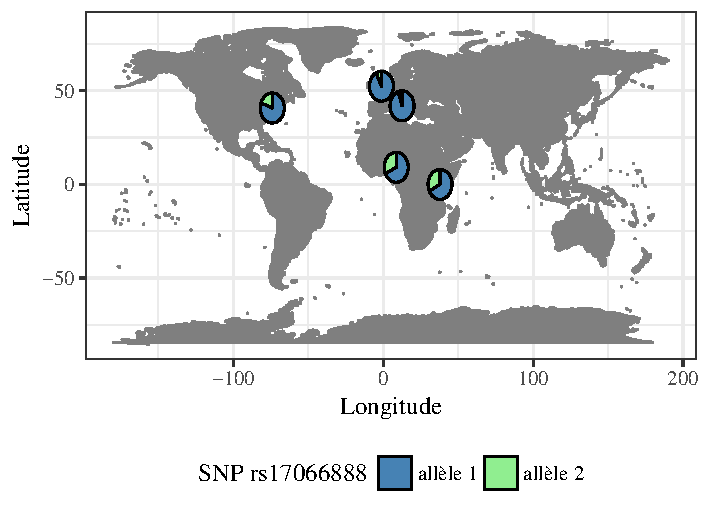
\includegraphics{./OUTPUT/Rplots/tess3_intro_freq.pdf}
\caption{{\bf Différenciation allélique entre des populations}. Distribution des
  allèles du SNP rs17066888 dans des populations européenne, africaine et
  afro-américaine.}
\label{fig:tess3_intro_freq}
\end{figure}

Une méthode très utilisée pour visualiser la structure de population est
l'analyse en composantes principales (ACP). Dans une population d'individus
structurée en \(K\) populations, il faut \(K-1\) axes principaux pour représenter la
structure de populations à partir de données génétiques \citep{Patterson_2006}.
Nous proposons d'illustrer ce résultat en calculant les deux premiers axes
principaux d'un échantillon de données de SNPs composé d'individus humains de
populations africaine, européenne et afro-américaine. Les deux premiers axes
principaux permettent de visualiser un groupe composé des individus européens et
deux groupes composés des individus africains. Les individus afro-américains
sont répartis entre les groupes européens et afro-américains (Figure
\ref{fig:tess3_intro_pca})

\begin{figure}[h]
\centering
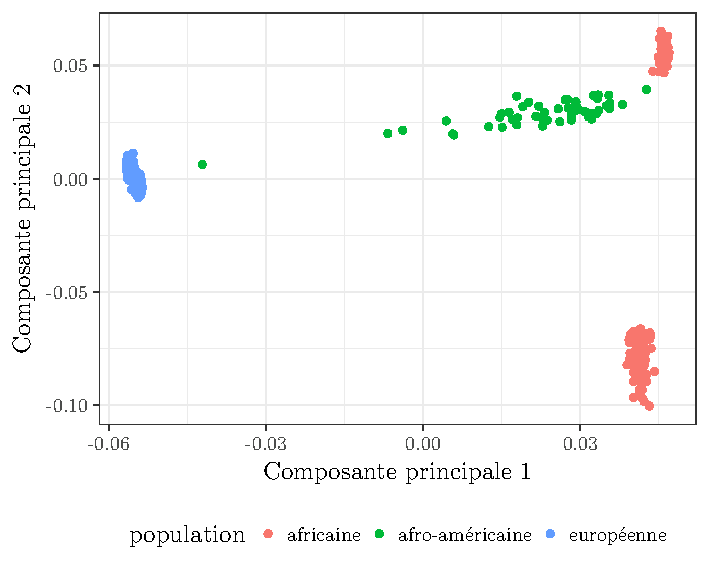
\includegraphics{./OUTPUT/Rplots/tess3_intro_pca.pdf}
\caption{{\bf Visualisation de la structure de population avec l'ACP.} Scores
  des deux premières composantes principales calculées sur des données de SNPs
  d'invidus humains de populations européenne, africaine et afro-américaine.}
\label{fig:tess3_intro_pca}
\end{figure}

Un modèle très utilisé pour étudier la structure génétique des populations à
partir de données de SNPs est celui du logiciel \texttt{structure} \citep{Pritchard2000}.
Dans ce modèle, nous supposons que le génome de chaque individu est la
combinaison de morceaux de génomes provenant de \(K\) clusters génétiques, aussi
appelé populations ancestrales. Dans le cadre de ce modèle, nous pouvons écrire
\begin{equation}
\label{eq:structure}
\Pr(\Y_{i,\ell} = j) = \sum_{k = 1}^{K} \matr{G}_{(d + 1)\ell + j, k} \Q_{i,k},
\end{equation}
où \(\Pr(\Y_{i,j} = d)\) est la probabilité d'observer l'allèle \(j\) au locus
\(\ell\) chez l'individu \(i\). Le terme \(\matr{G}_{(d + 1)\ell + j, k}\) représente la
fréquence d'apparition de l'allèle \(j\) au locus \(\ell\) dans le cluster génétique
\(k\). Le terme \(Q_{i,k}\) (appelé coefficient de métissage ou d'ascendance) est la
proportion de gènes de l'individu \(i\) provenant de la population \(k\). Les
coefficients d'ascendance et les fréquences d'allèles dans les clusters
génétiques sont respectivement rangés dans des matrices \(\Q\) et \(\matr{G}\). Afin
d'illustrer le modèle de \texttt{structure}, nous avons calculé les coefficients de
métissage sur le jeu de données utilisé précédemment pour illustrer l'ACP. Nous
avons utilisé le logiciel \texttt{snmf} qui permet de calculer des coefficients de
métissage à partir de données de SNPs avec \(K = 2\) clusters génétiques
\citep{Frichot_2015}. Les clusters génétiques trouvés par le logiciel \texttt{snmf} sont
européen et africain; tandis que les individus afro-américains ont des génomes
provenant des clusters génétiques africain et européen (Figure
\ref{fig:tess3_intro}). Il s'agit du résultat attendu au regard de l'histoire
démographique des individus afro-américains \citep{tishkoff2009genetic}.

\begin{figure}[h]
\centering
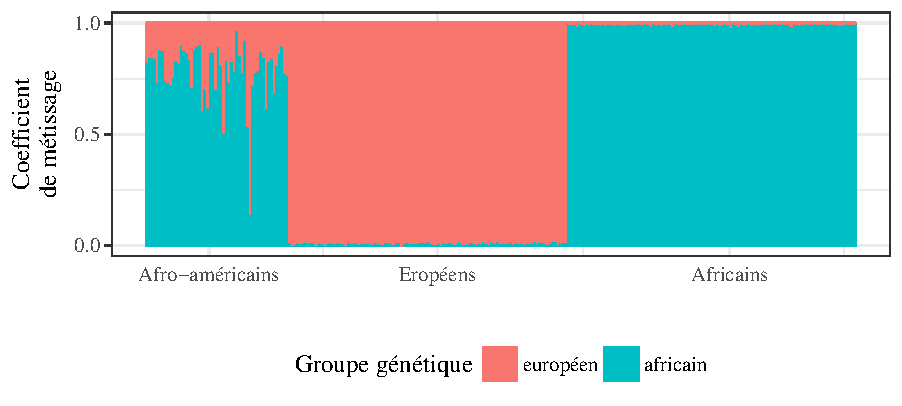
\includegraphics{./OUTPUT/Rplots/tess3_intro_barplot.pdf}
\caption{{\bf Coefficients de métissage.} Estimation par le logiciel
  \texttt{snmf} des coefficients de métissage pour un jeu de données composé
  d'individus humains provenant de populations européenne, africaine et
  afro-américaine.}
\label{fig:tess3_intro}
\end{figure}

\subsection{Méthodes d'estimation des coefficients d'ascendance}
\label{sec:orgb25d705}

Il existe de nombreuses méthodes pour estimer les coefficients d'ascendance à
partir de données génétiques. Le modèle du logiciel \texttt{structure} est bayésien et
l'inférence repose sur des méthodes d'échantillonnage de la loi a posteriori des
coefficients d'ascendance \citep{Pritchard2000}. D'autres méthodes visant à rendre
plus rapide l'inférence des matrices d'ascendance, minimisent la fonction
log-vraisemblance des paramètres d'ascendance génétique
\citep{Tang_2005,alexander2009admixture}. Certaines méthodes utilisent des
méthodes d'inférence variationnelle bayésiennes \citep{Raj_2014}. Des méthodes
très rapides, ne reposant pas sur une modélisation probabiliste, ont aussi été
proposées pour passer à l'échelle des grands jeux de données modernes
\citep{Frichot_2014,Popescu_2014}. Par ailleurs, de nombreuses méthodes utilisent
l'information spatiale individuelle afin d'améliorer l'estimation de
l'ascendance génétique et de localiser les clusters génétiques dans l'espace.
Des méthodes ont ajouté l'information géographique au modèle bayésien de
\texttt{structure} \citep{CHEN_2007,Corander2008,GUEDJ_2011}. Cependant, les méthodes
bayésiennes reposent sur de nombreuses hypothèses et passent plus difficilement
à l'échelle des grands jeux de données. Aucune méthode non basée sur un modèle
probabiliste n'a été proposée pour l'inférence spatiale des coefficients
d'ascendance. Nous résumons les méthodes d'inférence des coefficients
d'ascendance génétique dans la Table \ref{tab:org0629a90}

\rowcolors[]{2}{contiYellow!5}{contiYellow!20}
\begin{sidewaystable}[htbp]
\caption{\label{tab:org0629a90}
\textbf{Méthodes spatiales et non spatiales d'estimation de coefficients d'ascendance.} Les méthodes TESS3-AQP/APLS sont présentées dans cette thèse.}
\centering
\begin{tabular}{l|p{5cm}lp{5.5cm}|p{5.5cm}}
\hline
Méthode & Modèle & Spatiale & Algorithme & Référence\\
\hline
STRUCTURE & bayésien & non & MCMC & \citet{Pritchard2000,Falush1567}\\
FRAPPE & vraisemblance & non & EM & \citet{Tang_2005}\\
TESS & bayésien & oui & MCMC & \citet{CHEN_2007}\\
GENELAND & bayésien & oui & MCMC & \citet{phdGuedj}\\
BAPS & bayésien & oui & optimisation stochastique & \citet{Corander2008}\\
ADMIXTURE & vraisemblance & non & optimisation quasi-Newton alternée & \citet{alexander2009admixture,Alexander_2011}\\
fastStructure & bayésien & non & inférence variationnelle bayésienne & \citet{Raj_2014}\\
PSIKO & PCA & non & SVD & \citet{Popescu_2014}\\
sNMF & factorisation matricielle parcimonieuse & non & optimisation quadratique alternée avec projection & \citet{Frichot_2014}\\
TESS3-AQP & factorisation matricielle régularisée sur graphe & oui & optimisation quadratique alternée & \\
TESS3-APLS & factorisation matricielle régularisée sur graphe & oui & moindres carrés alternés projetés & \\
conStruct & bayésien & oui & MCMC & \citet{Bradburd189688}\\
\end{tabular}
\end{sidewaystable}
\rowcolors{2}{}{}

\section{Tests d'association}
\label{sec:orgae53d8b}
Un problème fondamental en science du vivant consiste à détecter les relations
de causalité qui existent entre des événements. En statistique, un événement est
modélisé par une variable aléatoire. Il est seulement possible de détecter des
liens statistiques entre les variables aléatoires; on parle alors d'étude de
corrélations. La corrélation renseigne sur les probabilités jointes des
variables aléatoires en question. Dans un cadre statistique, nous parlons de
tests d'association lorsque l'on cherche à identifier des corrélations entre des
variables aléatoires.

Les tests d'association sont très utilisés en génétique pour comprendre les
fonctions des gènes. Par exemple, on peut chercher quels SNPs sont corrélés à
une maladie pour comprendre les causes génétiques de celle-ci. Cependant, comme
nous l'avons vu dans la partie précédente, il existe de nombreux facteurs
responsables de la diversité génétique. Quand les facteurs de variation du
génome sont corrélés à la variable d'étude (la maladie par exemple), alors les
études d'association sont faussées. On observe en général une augmentation du
nombre de gènes associés à la variable d'étude. Une telle situation n'est pas
souhaitable car bien qu'il s'agisse de corrélations, il ne s'agit pas de
corrélations intéressantes pour l'étude biologique. Nous expliquons maintenant
plus en détail ce que sont les facteurs de confusion dans les études
d'association.

\subsection{Les facteurs de confusion}
\label{sec:org78f8559}
\label{orgd48b945}

Basées sur l'analyse de la corrélation, les études d'association sont
confrontées aux problèmes des facteurs de confusion et de la causalité. En effet
lorsque l'on détecte une corrélation entre deux variables, cela n'implique pas
nécessairement qu'il y a un lien de causalité entre celles-ci. Le lien de
causalité entre les deux variables peut être bien plus complexe et notamment
impliquer des liens avec d'autres variables non observées. En particulier, il
est possible de conclure à une association entre deux variables alors qu'elles
sont associées à une autre variable non considérée dans l'étude. On appelle
alors la variable non observée un facteur de confusion. La figure
\ref{fig:org4bbc538} illustre cette situation. Le problème des facteurs de
confusion est connu depuis longtemps. En effet, on le retrouve déjà dans
l'ouvrage \emph{The Design of Experiment} de Ronald Fisher qui introduisit entre
autre le concept d'hypothèse nulle en statistique \citep{fisher1937design}. Dans
cette thèse nous nous intéressons aux études d'association à très grande
échelle. Nous avons d'une part des observations de \(\Ycol\) variables sur \(\Yrow\)
individus rassemblées dans une matrice \(\Y\) de taille \(\Yrow \times \Ycol\), et
en général \(\Ycol\) est très grand devant \(\Yrow\). Nous avons d'autre part
l'observation d'une variable sur les mêmes \(\Xrow\) individus que l'on rassemble
dans une matrice \(\X\), de taille \(\Xrow \times 1\). L'objectif est alors de
trouver parmi les \(\Ycol\) variables \(\Y\) celles qui sont associées à \(\X\). Nous
supposons de plus qu'il existe un certain nombre de variables non observées qui
permettent d'expliquer les variations de \(\Y\). Ces variables non observées, que
l'on appellera variables latentes, sont potentiellement des facteurs de
confusion pour l'étude d'association entre les matrices \(\Y\) et \(\X\). Les
variables latentes sont potentiellement corrélées à \(\X\); il faut donc les
prendre en compte dans l'étude d'association.

\begin{figure}[htbp]
\centering
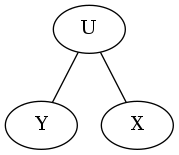
\includegraphics[width=5cm]{Figures/conf_factor.png}
\caption{\label{fig:org4bbc538}
\textbf{Graphe de corrélation entre la variable \(\Y\), la variable \(\X\) et le facteur de confusion \(\matr{U}\).} Dans cette situation si on ne prend pas en compte la variable \(\matr{U}\) dans l'étude d'association alors \(\X\) et \(\Y\) apparaîtront comme étant associées.}
\end{figure}

\subsection{Simulation numérique d'une association avec facteurs de confusion}
\label{sec:org23c297f}
\label{org6f0a320}

Dans cette partie nous proposons de montrer l'intérêt de prendre en
considération les facteurs de confusion dans les études d'association par une
simulation numérique. Pour cela nous simulons une variable explicative \(\X\) et
une variable latente \(\matr{U}\), de sorte que le coefficient de corrélation
entre les deux variables soit égal à \(0.6\). Nous simulons ensuite une matrice
de bruit gaussien de moyenne nulle et variance égale à 1, notée \(\E\). La matrice
des effets de la variable latente sur \(\Y\) est aussi simulée à l'aide de la loi
normale. Nous notons la matrice des effets latents \(\V\). La matrice des effets
de \(\X\) sur \(\Y\), notée \(\B\), est simulée de sorte que \(1 \%\) de ses lignes
soient non nulles. Enfin, la matrice des variables expliquées, \(\Y\), est calculée
telle que
\begin{equation} 
\Y = \matr{U} \V^{T} + \X \B^{T} + \E. 
\label{eq:model0}
\end{equation} 
Cette simulation correspond à une situation où \(1 \%\) des colonnes de \(\Y\) sont
associées à \(\X\). La variable latente \(\matr{U}\) est un facteur de confusion
pour cette étude d'association car elle est corrélée à la variable \(\X\).

Afin de détecter les variables expliquées associées à la variable explicative,
nous réalisons une régression linéaire de \(\Y\) par \(\X\). Nous effectuons une
seconde régression linéaire avec cette fois la variable \(\X\), ainsi que la
variable latente \(\matr{U}\), comme variables explicatives de la régression. Nous
réalisons un test de Student pour tester la nullité des coefficients associés à
la variable \(\X\) dans chacune des deux régressions. Quand on ne prend pas en
compte la variable latente, plus de \(40 \%\) des \pvalues sont inférieures à
\(10^{-15}\); alors que quand on prend en compte les facteurs latents, la
distribution des \pvalues est bien uniforme comme on s'y attend (Figure
\ref{fig:simu_intro}). En effet, on s'attend à une distribution uniforme des
\pvalues car la majorité des colonnes de \(\Y\) ne sont pas associées à la
variable \(\X\) (seulement \(1\%\) y sont associées par simulation). Dans le cas de
cette simulation il est impossible de ne pas prendre en compte la variable
latente; sans celle-ci on détecte presque la moitié des colonnes de \(\Y\) comme
étant associées à \(\X\).

\begin{figure}[!t]
\centering
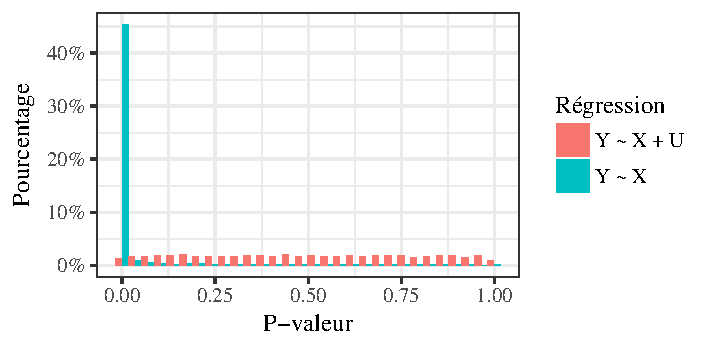
\includegraphics{./OUTPUT/Rplots/simu_intro.pdf}
\caption{{\bf Test de nullité des coefficients de la régression sans et avec le
    facteur de confusion.} Les données ont été simulées avec une variable
  latentes $\matr{U}$ corrélée avec la variable $\X$. }
\label{fig:simu_intro}
\end{figure}

\subsection{Méthodes de correction des facteurs de confusion pour les études d'association}
\label{sec:org1c76882}

Prendre en compte les facteurs latents est un problème important des études
d'association. Certaines méthodes utilisent l'analyse en composantes principales
pour estimer les facteurs de confusion et les intégrer aux tests de
significativité \citep{Rahmani_2016,Price_2006}. D'autres méthodes utilisent les
modèles mixtes afin de corriger les tests d'hypothèse pour les sources de
variation indésirable \citep{Kang_2008,Zhou_2014,Loh194944}. Récemment, de
nombreuses méthodes ont été proposées pour permettre d'estimer dans un même
modèle les effets des variables latentes et les effets des variables étudiées
pour l'association. La plupart de ces méthodes reposent sur l'équation
\eqref{eq:model0} que nous avons utilisée dans la partie précédente. Ces modèles
ont recu plusieurs noms dans la littérature : Latent Fator Mixed Models (LFMM)
\citep{Frichot_2013}, regression-based latent models (RLFM)
\citep{agarwal09_regres}, factor-augmented regression model
\cite{gerard2017empirical}, surrogate variable analysis (SVA)
\cite{article_Leek_Storey_2007}. Nous résumons dans le Table
\ref{tab:org773b2d1}, les méthodes reposant sur des modèles construits à
partir de l'équation \eqref{eq:model0} .

\rowcolors[]{2}{contiYellow!5}{contiYellow!20}
\begin{sidewaystable}[htbp]
\caption{\label{tab:org773b2d1}
\textbf{Méthodes reposant sur l'équation \ref{eq:model0} pour la correction des facteurs de confusion dans les études d'association.} Les méthodes ridgeLFMM et LassoLFMM sont présentées dans cette thèse. Les méthodes cate, sva-twostep et sva-riw sont présentées plus en détail dans la section \ref{orgb7a2d5c}.}
\centering
\begin{tabular}{p{3cm}|p{4.2cm}p{4cm}p{5cm}|p{4cm}}
\hline
Méthode & Modèle & Algorithme & Test d'hypothèse & Référence\\
\hline
sva-twostep & PCA et régression linéaire & moindres carrés ordinaire et SVD & test de Fisher & \citet{article_Leek_Storey_2007}\\
sva-irw & weighted-PCA et régression linéaire & moindres carrés ordinaire et \emph{weighted}-SVD & test de Fisher & \citet{article_Leek_Storey_2008}\\
RLFM & bayésien & Monte-Carlo EM & pas de test & \citet{agarwal09_regres}\\
famt & vraisemblance & EM & test de Student & \citet{friguet09_factor_model_approac_to_multip}\\
LFMM & bayésien & MCMC & test de wald, estimation de la variance par bootstrap bayésien & \citet{Frichot_2013}\\
cate & analyse factorielle et régression linéaire & EM ou SVD et estimation des moindres carrés généralisée & test basé sur la distribution asymptotique de l'estimateur des effets d'intérêt & \citet{wang2015confounder}\\
ridgeLFMM & factorisation matricielle avec régularisation \(L_{2}\) & SVD et estimation des moindres carrés régularisée en norme \(L_{2}\) & test de Student & \\
lassoLFMM & factorisation matricielle avec régularisation \(L_{1}\) & \emph{soft-thresholded} SVD et estimation des moindres carrés régularisée en norme \(L_{1}\) & test de Student & \\
MOUTHWASH / BACKWASH & régression linéaire et analyse factorielle & moindres carrés ordinaire et EM ou descente par coordonnées & \emph{adaptive shrinkage} (ASH) \citep{stephens16_false_discov_rates} & \citet{gerard2017empirical}\\
\end{tabular}
\end{sidewaystable}
\rowcolors{2}{}{}

\section{Résumé de la problématique}
\label{sec:orgd309411}

L'évaluation de l'ascendance génétique est un problème majeur en génétique des
populations. Des méthodes très efficaces ont été proposées pour l'estimation des
coefficients d'ascendance à partir de données génétiques. Cependant, l'estimation
de l'ascendance génétique en intégrant l'information spatiale a reçu moins
d'attention. Ainsi, afin de permettre l'étude des données génétiques modernes,
le développement de méthodes statistiques pour l'inférence de l'ascendance
génétique intégrant l'information spatiale est nécessaire.

Répondant à l'arrivée massive de données, le développement de méthodes pour les
études d'association à grandes échelles, est très actif en ce moment. Dans les
études d'association, un aspect très important est de détecter et corriger les
sources de variation indésirable pour l'étude. Chaque méthode utilise des
approches différentes et aucune ne s'est imposées comme étant la méthode de
référence. Dans le contexte actuel il est nécessaire de développer des
méthodes rapides et utilisables sur les données massives. Par ailleurs, une
comparaison des méthodes de correction pour les facteurs de confusion
permettrait de mieux comprendre les spécificités de chaque méthode.
\section{Contexte de la thèse}
\label{sec:org4eee06f}
Cette thèse a été financée par le LabEx PERSYVAL-Lab et co-encadrée par Olivier
François du laboratoire TIMC-IMAG et Olivier Michel du laboratoire GIPSA-lab.
Nos travaux ont principalement été réalisés au sein de l'équipe BCM (Biologie
Computationnelle et Mathématique). L'équipe BCM du laboratoire TIMC-IMAG est
spécialisée en étude de données génétiques et en développement de modèles
mathématiques pour les systèmes biologiques complexes. Les méthodes présentées
dans cette thèse sont donc dans la lignée des méthodes développées au sein de
l'équipe BCM. Ainsi, les logiciels que nous avons développés dans cette thèse
viennent compléter les logiciels produits par l'équipe BCM. Nous parlons en
particulier de \texttt{TESS} 2.3, un logiciel d'inférence spatiale de la structure
génétique des populations \citep{Durand_2009}; ainsi que de \texttt{LEA}, un package R
proposant une suite de fonctions dédiées aux études d'association génomique
\citep{Frichot_2015}.

\section{Objectifs de la thèse}
\label{sec:org881ceae}

La génétique produit beaucoup de données grâce aux technologies de séquençage
toujours plus efficaces. Cette affluence de données pose de nouveaux problèmes
aux statisticiens. L'objectif de cette thèse de doctorat est d'améliorer les
outils statistiques qui permettent aux biologistes de répondre à des questions
concrètes sur le vivant. Dans cette thèse nous nous sommes intéressés à deux
problématiques en analyse de données génétiques : l'estimation de la structure
génétique de population et les études d'association. L'accent a été mis sur la
complexité des algorithmes développés afin qu'ils soient applicables aux données
génétiques modernes. De plus, l'importance a été placée aussi bien sur le
développement mathématique des méthodes que sur leur implémentation
informatique. Afin que nos méthodes statistiques soient utilisables par la
communauté scientifique, il a été important de rendre accessibles des
implémentations informatiques efficaces des nouvelles méthodes statistiques.

\section{Résumé des résultats principaux}
\label{sec:orga44a34d}

Dans le cadre de cette thèse, nous avons proposé plusieurs méthodes reposant sur
des problèmes de factorisation matricielle. Nos méthodes ont été implémentés
dans deux packages R : \texttt{tess3r} et \texttt{lfmm}. Le package \texttt{tess3r} contient les
algorithmes AQP et APLS d'inférence de l'ascendance génétique en incluant
l'information spatiale. Le package \texttt{lfmm} contient les algorithmes lassoLFMM et
ridgeLFMM d'estimation des facteurs de confusion pour corriger les études
d'association.


\subsection{\texttt{tess3r}}
\label{sec:org2ca1207}

Dans le package \texttt{tess3r}, nous avons développé des algorithmes d'estimation
rapide des coefficients de métissage à partir de données génétiques et
géographiques. Les algorithmes reposent sur un problème de factorisation de la
matrice génétique. L'objectif est de factoriser la matrice génétique en le
produit d'une matrice des coefficients d'ascendance et d'une une matrice des
fréquences d'allèle dans les clusters génétiques. Pour inférer les matrices
d'ascendance nous avons utilisé une approximation des moindres carrés.
L'information spatiale est ajoutée à la fonction objectif au moyen d'une
régularisation sur la matrice des coefficients de métissage. La régularisation
spatiale permet d'ajouter l'hypothèse que des individus proches ont plus de
chance de partager des ancêtres communs, que des individus éloignés. Afin
d'estimer les matrices d'ascendance, nous avons proposé deux algorithmes appelés
AQP et APLS. Nos algorithmes diffèrent dans les approximations qu'ils font pour
diminuer la complexité algorithmique. Plus précisément, nous avons d'une part
l'algorithme AQP qui alterne des résolutions de problèmes d'optimisation
quadratique. Le corollaire 2 établi par \citet{Grippo_2000} permet de montrer la
convergence de l'algorithme AQP vers un minimum local de la fonction objectif.
Nous avons d'autre part, l'algorithme APLS pour lequel nous avons supprimé les
contraintes des problèmes d'optimisation quadratique. Cela permet d'alterner la
résolution de problèmes des moindres carrés régularisés par une norme \(L_{2}\).
Ainsi, la complexité de l'algorithme APLS augmente linéairement avec le nombre
d'individus dans l'échantillon. De plus, nous avons mis en place un test de
détection de l'adaptation locale. La statistique de test est calculée à partir
des estimations spatiales des matrices d'ascendance génétique.

En utilisant des simulations de coalescents, nous avons montré que les deux
algorithmiques AQP et APLS retournent des résultats avec la même précision
statistique. Toujours sur des simulations de coalescents, nous avons montré que
nos algorithmes reproduisent les mêmes erreurs statistiques que le logiciel
\texttt{TESS} 2.3 \cite{CHEN_2007}. Le logiciel \texttt{TESS} 2.3 permet également l'estimation
des coefficients de métissage à partir de données génétiques et géographiques mais
en utilisant un modèle bayésien. Sur ces simulations, nos algorithmes étaient 10
à 100 fois plus rapides que le logiciel \texttt{TESS} 2.3.

Pour mesurer le bénéfice de l'utilisation d'algorithmes spatiaux, nous avons
comparé les erreurs statistiques observées pour les algorithmes spatiaux avec
celles observées pour un algorithme non spatial \texttt{snmf} \cite{Frichot_2014}. Dans
nos expériences numériques, les erreurs des méthodes spatiales sont inférieures
à celles observées avec des méthodes non spatiales. De plus, les algorithmes
spatiaux ont permis de détecter une structure de population plus subtile.

Enfin, nous avons illustré l'utilisation de notre package R sur un millier de
génotypes \emph{A.thaliana}, chacun incluant plus de 210k SNPs. Notre méthode a
permis d'exiber la structure de population de l'espèce \emph{A.thaliana} en Europe.
Par ailleurs, nous avons appliqué les tests de neutralité afin d'effectuer un
balayage du génome pour la sélection dans des écotypes européens de l'espèce
végétale \emph{A.thaliana}. Le scan du génome a confirmé la preuve de la sélection
des gènes liés à la floraison \emph{CIP4.1}, \emph{FRI} et \emph{DOG1} différenciant la
Fenno-Scandinavie du nord-ouest de l'Europe \citep{Horton_2012}.

\subsection{\texttt{lfmm}}
\label{sec:orgcd6c9a3}
Dans le package \texttt{lfmm}, nous avons développé des algorithmes qui permettent
d'estimer les variables latentes afin de corriger les études d'association pour
les facteurs de confusion. Nous avons proposé une fonction objectif basée sur
l'approximation des moindres carrés de l'égalité \eqref{eq:model0} du modèle mixte
à facteurs latents. Le modèle consiste à expliquer les variations des variables
étudiées par la somme de deux effets : l'effet des variables latentes et l'effet
des variables explicatives (ces dernières sont aussi appelées covariables).
L'attache aux données de la fonction objectif a été construite à partir de
l'approximation des moindres carrés de l'égalité \eqref{eq:model0}. Nous avons
montré que le terme d'attache aux données ne permet pas à lui seul de définir
des estimateurs de manière univoque pour notre problème. Ainsi, nous avons
proposé d'ajouter un terme de régularisation portant sur les effets des
variables explicatives. Nous avons appelé nos méthodes ridgeLFMM, pour la
régularisation \(L_{2}\) et lassoLFMM, pour la régularisation \(L_{1}\).
L'algorithme ridgeLFMM utilise la formule du minimum global de la fonction
objectif des moindres carrés régularisée en norme \(L_{2}\). Nous avons apporté la
démonstration de cette formule. Pour l'algorithme lassoLFMM, nous avons proposé
une méthode alternée de descente par blocs de coordonnées. Les travaux de
\citet{Tseng_2001} permettent de démontrer la congergence de l'algorithme
lassoLFMM vers le minimum global de sa fonction objectif. Cependant, nous avons
proposé une preuve adaptée au résultat de convergence de notre algorithme.

Pour évaluer la capacité de nos méthodes à corriger les études d'association
pour les facteurs de confusion, nous avons réalisé des simulations à partir d'un
jeu de données réelles de génotypes humains. Nous avons ajouté à la comparaison
une méthode de référence qui ne prend pas en compte les facteurs latents. Nous
avons aussi comparé les méthodes de la littérature reposant sur le même modèle
de régression avec facteur latent que nos méthodes : cate, sva-irw et
sva-twostep. Nous avons également considéré la méthode calculant les facteurs
latents à l'aide de l'ACP. Ces simulations nous ont permis de montrer que nos
méthodes ridgeLFMM et lassoLFMM ont la même puissance que la méthode oracle qui
connait les variables latentes de la simulation. De plus, les statistiques
\pvalues obtenues avec nos méthodes sont correctement calibrées. Nous avons
observé que la méthode cate obtenait des performances très proches de celles de
nos méthodes sur toutes les simulations considérées.

Enfin, nous avons illustré l'utilisation de nos méthodes sur des études
d'association pour des données réelles. Sur les données réelles, nous montrons
que nos méthodes permettent de retrouver les associations découvertes par
d'autres études. De plus, nous observons dans ces études que malgré les
ressemblances conceptuelles entre les méthodes, les associations découvertes
peuvent varier largement d'une méthode à l'autre. Cela met en avant la nécessité
d'utiliser plusieurs méthodes dans les études d'association, ainsi que d'être
prudent dans les interprétations.

\chapter[Inférence spatiale des coefficients de métissage]{Inférence des coefficients de métissage à l'aide de données géographiques}
\label{sec:org77b2612}
\label{orgbd1de0b}
\section{Résumé}
\label{sec:orgd20fd47}

L'évaluation précise de la répartition de l'ascendance génétique dans l'espace
géographique est l'une des principales questions abordées par les biologistes de
l'évolution. Cette question a été communément abordée par l'application de
programmes d'estimation bayésiens permettant à leurs utilisateurs d'estimer les
proportions individuelles de métissage et les fréquences alléliques parmi les
populations ancestrales putatives. Suite à l'explosion des technologies de
séquençage à haut débit, plusieurs algorithmes ont été proposés pour faire face
au fardeau de calcul généré par les données massives dans ces études. Dans ce
contexte, l'intégration de la proximité géographique dans les algorithmes
d'estimation de l'ascendance est un défi statistique et computationnel ouvert.
Dans ce chapitre, nous introduisons de nouveaux algorithmes qui utilisent
l'information géographique pour estimer les proportions d'ascendance et les
fréquences génotypiques ancestrales à partir des données génétiques de la
population étudiée. Nos algorithmes combinent les méthodes de factorisation
matricielle et les statistiques spatiales pour fournir des estimations des
matrices d'ascendance basées sur l'approximation des moindres carrés. Nous
démontrons le bénéfice de l'utilisation d'algorithmes spatiaux grâce à des
simulations numériques, et nous fournissons un exemple d'application de nos
nouveaux algorithmes à un ensemble d'échantillons référencés spatialement pour
les espèces végétales \emph{Arabidopsis thaliana}. Sans perte de précision
statistique, les nouveaux algorithmes présentent des temps d'exécution beaucoup
plus courts que ceux observés pour les méthodes spatiales développées
antérieurement. Nos algorithmes sont implémentés dans le package R, \texttt{tess3r}.

\section{Introduction}
\label{sec:org9882707}
\label{org1e0e097}

Représenter la structure génétique de population est une étape importante dans
l'étude de données génétiques. Les données génétiques sont volumineuses et
multivariées. La structure génétique des populations fournit une représentation
synthétique qui permet de visualiser la variation génétique induite par la
stratification en populations. La stratification en populations fournie des
informations sur l'histoire et l'évolution démographique de l'espèce étudié
\citep{Li_2008}. Il est également indispensable de l'utiliser comme facteur de
correction dans les études d'association à un phénotype, un gradient
environnemental ou encore une maladie \citep{marchini2004effects}. De même, il
existe de nombreuses applications en médecine génétique nécessitant de connaître
la structure de populations, comme par exemple le calcul d'un score de risque
génétique pour une maladie \citep{Wray_2013}. Enfin, l'étude de la répartition en
population d'une espèce dans son habitat est une étape clé en génétique du
paysage \citep{Fran_ois_2015}.

Pour modéliser la structure génétique des populations, nous supposons que le
génome de chaque individu est la combinaison de morceaux de génomes provenant de
\(K\) clusters génétiques; les clusters génétiques sont aussi appelé populations
ancestrales \citep{Pritchard2000}. Dans chaque cluster génétique, l'objectif est
d'estimer les fréquences d'allèle pour chaque SNPs. Pour chaque individu, il
faut estimer la proportion de son génotype qui provient de chaque cluster
génétique. Les proportions sont appelées coefficients de métissage individuel,
aussi appelés coefficients d'ascendance.

\subsection{Méthodes d'inférence des coefficients de métissage}
\label{sec:orgd4b9a55}
L'inférence des coefficients de métissage a été largement étudiée et il existe
de nombreuses méthodes. On distingue deux types d'approche : les approches
reposant sur un modèle probabiliste et les approches fondées sur l'optimisation
d'une fonction objectif.

Parmi les approches reposant sur un modèle probabiliste, on compte le logiciel
\texttt{structure} proposé par \citet{Pritchard2000} qui a introduit le modèle de
structure génétique de population dont nous avons parlé dans l'introduction.
L'accès à des données génétiques de plus en plus massives a provoqué l'émergence
de plusieurs algorithmes plus rapides que celui de \texttt{structure}. En effet, le
logiciel \texttt{structure} implémente un algorithme d'échantillonnage de Monte-Carlo
pour estimer la distribution a posteriori des coefficients de métissage et des
fréquences d'allèle dans les clusters génétiques. Cependant les algorithmes de
Monte-Carlo ne passent pas à l'échelle des grands jeux de données génétiques
modernes. Il a été proposé des améliorations du logiciel \texttt{structure} reposant
sur une fonction de vraisemblance définie pour la matrice des coefficients de
métissage et les fréquences d'allèle dans les clusters. L'estimation est
effectuée en maximisant la fonction log-vraisemblance. Une première amélioration
de l'algorithme \texttt{structure} est fondée sur un algorithme EM (Expectation
Maximisation) maximisant la fonction de vraisemblance \citep{Tang_2005}. Des
algorithmes de vraisemblance plus récents sont implémentés dans les programmes
\texttt{admixture} et \texttt{fastStructure} \citep{Alexander_2011,Raj_2014}.

Dans les approches reposant sur l'optimisation d'une fonction objectif, les
coefficients de métissage sont estimés à l'aide de méthodes de moindres carrés
ou d'analyse factorielle. Pour estimer les matrices des coefficients de
métissage et de fréquence d'allèle dans les clusters, \citet{Engelhardt_2010}
proposent d'utiliser une analyse parcimonieuse à facteurs; \citet{Frichot_2014}
utilisent des algorithmes de factorisation de matrice non négative;
\citet{Popescu_2014} utilisent l'analyse en composantes principales. Ces méthodes,
reposant sur des problèmes d'optimisation, permettent de reproduire avec
précision les résultats des approches considérant une fonction de vraisemblance
\citep{Frichot_2014}. En outre, cette catégorie de méthodes fournit des
algorithmes qui sont généralement plus rapides que ceux des méthodes reposant
sur un modèle probabiliste.

\subsection{Méthodes d'inférence des coefficients de métissage à l'aide de données géographiques}
\label{sec:org5369fb9}

Dans la nature, les individus d'une espèce évoluent dans un environnement
géographique. Les clusters génétiques, identifiés par les méthodes d'estimation
de la structure génétique des populations, sont induits par les pressions
évolutives qui s'opèrent dans l'environnement géographique de l'espèce. Les
clusters génétiques peuvent par exemple être générés par l'isolation des
populations à cause d'une mer les séparant ou bien des différences d'altitude
entre celles-ci. L'étude réalisée par \citet{Novembre_2008} a montré qu'il est
possible de prédire la position des individus à partir de l'étude de la
structure génétique des populations. De nombreuse méthodes ont permis
d'améliorer la prédiction de la position géographique des individus à partir du
génome \citep{Baran_2013,Yang_2012,Bhaskar_2016,Ra_ola_2014}. Si la structure
génétique des populations permet de prédire la position spatiale des individus,
alors il est possible d'améliorer l'estimation de la structure génétique des
populations en utilisant l'information géographique. Cette idée a été exploitée
pour améliorer le modèle bayésien de \texttt{structure} en intégrant des données
géographiques dans la distribution a priori des coefficients de métissage
\citep{CHEN_2007,Corander2008}. Les algorithmes spatiaux fournissent des
estimations de la structure de population plus robustes que des algorithmes non
spatiaux qui peuvent conduire à des estimations biaisées du nombre de clusters
\citep{Durand_2009}. Certaines méthodes bayésiennes sont basées sur des
algorithmes de Monte-Carlo de chaîne de Markov qui nécessitent beaucoup de
calcul \citep{FRAN_OIS_2010}. Ainsi, les méthodes existantes d'estimation des
coefficients d'ascendance à l'aide de données géographiques ne sont pas adaptées
aux grands jeux de données modernes.

\subsection{Plan du chapitre}
\label{sec:org4a8173c}

Dans ce chapitre, nous présentons une nouvelle méthode pour l'estimation des
coefficients individuels de métissage fondée sur des données géographiques et
génétiques. Cette méthode repose sur un problème de factorisation de matrices
avec des contraintes convexes et une régularisation sur un graphe spatial. Nous
proposons deux algorithmes qui résolvent le problème de factorisation. Le
premier algorithme repose sur un algorithme d'optimisation quadratique alternée
(AQP pour alternated quadratic programing), l'autre sur un algorithme des
moindres carrés alternés projetés (APLS pour alternated projected least square).
Le terme alterné dans les deux algorithmes fait référence au fait que l'on
alterne une étape d'optimisation, selon la matrice des coefficients de
métissage, puis la matrice des fréquences de génotypes ancestraux. L'algorithme
AQP a un fondement théorique bien établi par \citet{Bertsekas_1997}; ce n'est pas
le cas de l'algorithme APLS. En utilisant des simulations coalescentes, nous
montrons que les estimations calculées par l'algorithme APLS sont de bonnes
approximations des solutions de l'algorithme AQP. De plus, nous montrons que les
performances de l'algorithme APLS s'élèvent aux dimensions des jeux de données
modernes. Sur des simulations, nous montrons que l'erreur statistique fournis
par APLS est du même ordre que l'erreur obtenue avec le logiciel \texttt{TESS} 2.3; ce
logiciel implémente une méthode bayésienne pour l'inférence spatiale de la
structure génétique des population. Toujours sur des simulations, nous montrons
que notre algorithme spatial APLS estime mieux la structure de population que la
méthode sNMF. L'algorithme de sNMF repose aussi sur un problème de factorisation
de matrice mais n'utilise pas l'information spatiale. Enfin, nous présentons
l'application de nos algorithmes aux données d'écotypes européens de l'espèce
végétale \emph{Arabidopsis thaliana}, pour lesquelles des données géographiques
individuelles et génétiques sont disponibles \citep{Horton_2012}.

\section{Nouvelles méthodes d'estimation des coefficients de métissage}
\label{sec:orgb222cf4}
Dans cette section, nous présentons deux nouveaux algorithmes d'estimation de la
structure génétique des populations qui intègrent l'information de proximité
géographique.

\subsection{Matrices d'ascendance génétique}
\label{sec:org1e2088c}

Nous considérons une matrice de génotype, \(\Y\), enregistrant des données de \(n\)
individus à \(p\) locus polymorphes pour une espèce ayant une ploïdie de \(d\),
c'est-à-dire qui possède un génome composé de \(d\) exemplaires de chaque
chromosome. Pour les SNPs autosomiques\footnote{Les SNPs autosomiques sont les SNPs des chromosomes autosomes
ou homologue. Les chromosomes autosomes sont formés de paires dont les membres
ont la même forme, mais diffèrent des autres paires dans une cellule diploïde.
Chez l'humain, on compte 22 paires de chromosomes homologues.} dans un organisme
diploïde, le génotype au locus \(\ell\) est un nombre entier, 0, 1 ou 2,
correspondant au nombre d'allèles de référence observé à ce locus. Dans nos
algorithmes nous utilisons des formes disjonctives introduites par
\citet{Frichot_2014} pour coder les génotypes. Par exemple pour un organisme
diploïde, le nombre d'allèles observés à chaque locus \(,0,1,2\) est encodé comme
\(100\), \(010\) et \(001\). Pour les organismes \(d\text{-ploïde}\), il existe \((d + 1)\)
génotypes possibles à chaque locus, et chaque valeur est encodée sous une forme
disjonctive unique.

En utilisant la même approche que \citet{Frichot_2014}, si l'on suppose qu'il y a
\(K\) clusters génétiques, nous cherchons à décomposer la matrice \(\Y\) en une
matrice de coefficients de métissage \(\Q\), de taille \(n \times K\) et une matrice
de fréquences de génotypes dans les \(K\) clusters génétiques \(\mathbf{G}\), de taille \(p
\times K\). Nous notons \(\Q_{i,k}\) le coefficient de métissage de l'individu \(i\)
pour le cluster \(k\). Nous avons de plus
\begin{equation}
\label{eq:QConst}
\Q \geq 0 \, , \quad \sum_{k=1}^K {\bf Q}_{i,k} = 1.
\end{equation}
Nous notons \(\mathbf{G}_{(d + 1)\ell + j, k}\) la fréquence du génotype \(j\) au locus \(\ell\)
dans le cluster \(k\) et nous avons
\begin{equation}
\label{eq:GConst}
\mathbf{G} \geq 0 \, , \quad \sum_{j=0}^{d} {\bf G}_{(d+1)\ell + j, k} = 1.
\end{equation}
Enfin, nous voulons estimer les matrices \(\Q\) et \(\mathbf{G}\) en factorisant la matrice
de génotype de la façon suivante
\begin{equation}
\label{eq:tess3:Y}
\Y = \Q \mathbf{G}^{T}.
\end{equation}
Ainsi le problème d'inférence peut être résolu en utilisant les méthodes de
factorisation de matrices non négatives avec en plus les contraintes convexes
décrites par les équations \eqref{eq:QConst} et \eqref{eq:GConst}
\citep{lee1999learning,Cichocki2009}. Dans la suite, nous utiliserons les notations
\(\DQ\) et \(\DG\) pour représenter les ensembles formés à partir des contraintes
sur les matrices \(\Q\) et \(\mathbf{G}\).
\subsection{Information géographique}
\label{sec:org174cea9}
L'information géographique est introduite dans le problème de factorisation de
matrice en utilisant des poids entre les individus. Les poids sont utilisés pour
imposer une contrainte de régularité de l'estimateur des coefficients de
métissage sur l'espace géographique. En effet, nous souhaitons que des individus
proches dans l'espace géographique aient des coefficients de métissage proches.
Les poids sont définis à partir des coordonnées géographiques des individus que
l'on note \(x_{i}\) pour chaque individu \(i\). Nous attribuons aux individus
proches dans l'espace un poids plus grand que pour des individus éloignés. Les
poids sont calculés en construisant un graphe complet pondéré entre les
individus. Entre chaque individu \(i\) et \(j\), nous construisons la matrice des
poids du graphe \(\W\) de la manière suivante
\begin{equation}
\label{eq:tess3Graph}
\W_{i,j} = \exp( - {\rm dist}( x_i, x_j )^2/ \sigma^2),
\end{equation}
où la fonction \({\rm dist}( x_i, x_j)\) définit une distance entre
les coordonnées géographiques \(x_{i}\) et \(x_{j}\) des individus d'indice \(i\) et \(j\). 

Ensuite, nous introduisons la matrice laplacienne associée à la matrice des poids
géographiques \(\W\). La matrice laplacienne est définie de la manière suivante
\begin{equation}
\label{eq:tess3Laplace}
\Laplacienne = \D - \W,
\end{equation}
où \(\D\) est la matrice diagonale tel que 
\begin{equation}
\label{eq:tess3Diag}
\left\{ \D_{,i,i} \right\}_{i = 1..n}= \left\{\sum_{j = 1}^n \W_{i,j}\right\}_{i = 1..n}.
\end{equation}
Par le calcul, \citet{DengCai2011} ont montré que 
\begin{equation}
\label{eq:tess3Reg}
{\rm Tr} (\Q^{T} \Laplacienne \Q)  = \frac{1}{2} \sum_{i,j = 1}^n  \W_{i,j}  \| \Q_{i,.} - \Q_{j,.} \|^2.
\end{equation}
où \(\mathrm{Tr}\), la trace, est la fonction qui renvoie la somme des valeurs
diagonales d'une matrice carrées. Dans notre approche, nous supposons que les
individus géographiquement proches ont plus de chance d'avoir des ancêtres
communs que des individus éloignés. Ainsi nous utilisons le terme défini par
l'équation \eqref{eq:tess3Reg} pour régulariser l'estimateur de la matrice des
coefficients de métissage \(\Q\).

\subsection{Problèmes d'optimisation des moindres carrés}
\label{sec:orgcdc83de}
L'estimation des matrices \(\Q\) et \(\mathbf{G}\) à partir de la matrice de génotype \(\Y\)
est réalisée en optimisant la fonction suivante
\begin{equation}
\mathcal{L}(\Q, \mathbf{G}) =   \|  {\bf Y} - {\bf QG}^T \|^2_{\rm F} +  \alpha {\rm Tr} (\Q^{T} \Laplacienne \Q), 
\label{eq:tess3LS}
\end{equation}
où la matrice \(\Q\) appartient à \(\DQ\), l'ensemble définie par les contraintes
\eqref{eq:QConst}, et la matrice \(\mathbf{G}\) appartient à \(\DG\), l'ensemble définie par les
contraintes \eqref{eq:GConst}. La notation \(\| \matr{M} \|_{\rm F}\) désigne la norme
de Frobenius de la matrice \(\matr{M}\). Le paramètre de régularisation \(\alpha\)
contrôle la régularité des estimations des coefficients de métissage dans
l'espace géographique. Les grandes valeurs de \(\alpha\) impliquent que les
coefficients de métissage aient des valeurs proches pour les individus
géographiquement proches.

\subsection{Algorithme d'optimisation quadratique alternée (AQP)}
\label{sec:orgff24e0c}

Nous remarquons que les polyèdres \(\DQ\) et \(\DG\) sont des ensembles convexes et
que la fonction \(\LS\) définie par l'équation \eqref{eq:tess3LS}, est convexe par
rapport à chaque variable \(\Q\) ou \(\mathbf{G}\) lorsque l'autre est fixée. Nous pouvons
ainsi appliquer l'algorithme de descente par blocs de coordonnées au problème
afin de trouver un minimum local de la fonction \(\LS\). L'algorithme de descente
par blocs de coordonnées consiste à alterner des étapes d'optimisation selon
chacune des coordonnées de la fonction à optimiser (Figure
\ref{fig:coordinate_descente}). Cet algorithme converge vers un minimum local
quand la fonction objectif est convexe et définie sur un ensemble convexe
\citep{Bertsekas_1997}. Le problème d'optimisation selon \(\mathbf{G}\), quand \(\Q\) est fixé,
est un problème d'optimisation quadratique. Il en va de même quand on échange
les rôles de \(\mathbf{G}\) et \(\Q\), c'est pour cela que l'algorithme est dit
d'optimisation quadratique alternée (AQP).

\begin{figure}[t]
\centering
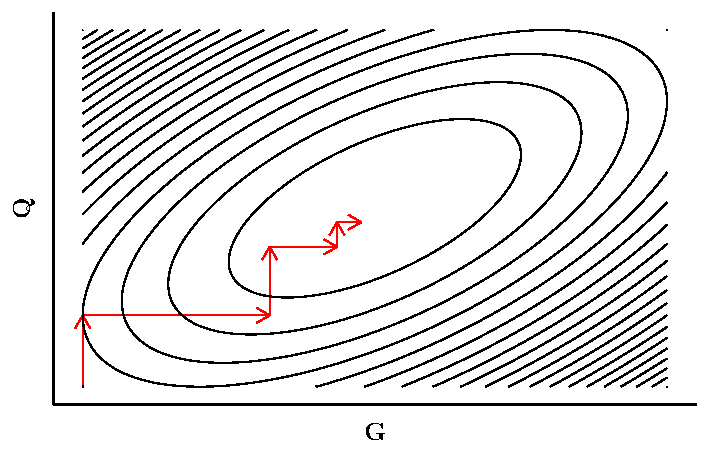
\includegraphics{./OUTPUT/Rplots/coordinate_descente.pdf}
\caption{{\bf Illustration de l'algorithme de descente par blocs de
    coordonnées.}}
\label{fig:coordinate_descente}
\end{figure}

L'algorithme APQ commence à partir de valeurs initiales pour les matrices
\(\mathbf{G}\) et \(\Q\), et alterne deux étapes d'optimisation. La première étape
calcule la matrice \(\mathbf{G}\) tandis que la matrice \(\Q\) est fixée. Nous
supposons que \(\Q\) est fixée et écrivons \(\mathbf{G}\) sous une forme vectorielle
comme ceci
\begin{equation*} 
g = {\rm vec}(\mathbf{G}) \in \mathbb{R} ^ {K(d +1)p}.
\end{equation*}
La première étape de l'algorithme résout le problème d'optimisation
quadratique suivant 
\begin{equation}
\begin{aligned}
\underset{g \in \DG}{\min}  ( -2  v^T_Q \, g + g^T \D^{Q} g ) ,
\end{aligned}
\label{eq:AQPg}
\end{equation}
où \(\D^{Q} = \Id_{(d + 1) p} \otimes \Q^T \Q\) et \(v_Q = {\rm vec} (\Q^T \Y)\).
Ici, \(\otimes\) désigne le produit Kronecker et \(\Id_{d}\) est la matrice identité
de taille \(d\). La structure en blocs de la matrice \(\D^{Q}\) nous permet de
décomposer le problème \eqref{eq:AQPg} en \(p\) problèmes de programmation
quadratiques indépendants à \(K(d + 1)\) variables.

Pour la deuxième étape de l'algorithme, nous considérons que \(\mathbf{G}\) est la
valeur obtenue après la première étape de l'algorithme, et écrivons \(\Q\) sous
une forme vectorielle
\begin{equation}
q = {\rm vec}(\Q) \in \mathbb{R}^{nK} 
\end{equation}
La deuxième étape résout le problème de programmation quadratique suivant
\begin{equation}
\begin{aligned}
\underset{q \in \DQ}{\min} ( -2 v^T_G \, q + q^T \D_G q ) ,
\end{aligned}
\label{eq:AQPq}
\end{equation}
où \(\D_G = \Id_{n} \otimes \mathbf{G}^T \mathbf{G} + \alpha \Laplacienne \otimes \Id_K\) et \(v_G
= {\rm vec}(\mathbf{G}^T \Y^T)\). Contrairement au problème \eqref{eq:AQPg} de la première
étape, le problème \eqref{eq:AQPq} ne peut pas être séparé en plus petits
problèmes. Ainsi, la deuxième étape de l'algorithme AQP nécessite de résoudre un
problème de programmation quadratique à \(n K\) variables; cela peut être très long
pour les jeux de données avec beaucoup d'individus. Nous alternons ces deux
étapes jusque convergence de l'algorithme AQP en un minimum local de \(\LS\).

Nous pouvons énoncer le résultat de convergence suivant.
\begin{theorem}
\label{orge8df024} L'algorithme AQP qui alterne les étapes d'optimisation des
problèmes \eqref{eq:AQPg} et \eqref{eq:AQPq} converge vers un minimum local de la
fonction \(\LS\) définie par l'équation \eqref{eq:tess3LS}.
\end{theorem}

\begin{proof}
La fonction \(\LS\) définie par l'équation \eqref{eq:tess3LS} est convexe par
rapport à \(\Q\) quand \(\mathbf{G}\) est fixé et inversement. De plus les ensembles
de définition \(\DQ\) et \(\DG\) sont convexes. Donc, d'après le corollaire 2 établi
par \citet{Grippo_2000}, tout point limite de l'algorithme AQP converge vers un
point de minimum local de la fonction \(\LS\).
\end{proof}

\subsection{Algorithme des moindres carrés alternés projetés (APLS)}
\label{sec:orgc0eb398}
Dans cette partie nous présentons l'algorithme APLS de calcul d'un minimum local
de la fonction \(\LS\) définie par l'équation \eqref{eq:tess3LS}. Contrairement à
AQP, il n'y a pas de résultat qui garantisse la convergence de d'APLS vers un
minimum local de la fonction \(\LS\). Cependant, l'algorithme APLS a une
complexité algorithmique plus faible que l'algorithme AQP. L'algorithme APLS
commence par initialiser au hasard les matrices \(\Q\) et \(\mathbf{G}\) puis alterne deux
étapes. La matrice \(\Q\) est calculée pendant que la matrice \(\mathbf{G}\) est fixé et
vice versa. 

La première étape de calcul de \(\mathbf{G}\) consiste à calculer
\begin{equation}
\label{eq:tess3:apls:g}
{\bf G}^\star = \arg \min  \|  {\bf Y} - {\bf QG}^T \|^2_{\rm F} \, .
\end{equation}
Cette étape peut être séparée en \((d+1) p\) (le nombre de colonnes de \(\Y\))
problèmes indépendants. De plus, cette opération peut être parallélisée. Ensuite
nous projetons \(\mathbf{G}^{\star}\) sur le polyèdre \(\DG\). 

Pour la seconde étape de calcul de la matrice \(\Q\), nous commençons par calculer
la matrice des vecteurs propres de la matrice laplacienne \(\laplacienne\) que
nous notons \(\matr{U}\), ainsi que la matrice diagonale \(\LapVp\) formée des valeurs
propres de \(\Laplacienne\). Comme la matrice laplacienne est symétrique et
positive ses valeurs propres sont des nombres réels non-négatifs. D'après le
théorème spectral nous avons
\begin{equation}
\Laplacienne = \matr{U}^T \LapVp \matr{U}.
\end{equation}
Après cette opération nous projetons la matrice des données \(\Y\) sur la base des
vecteurs propres de la façon suivante
\begin{equation}
\label{eq:3}
\mathcal{P}(\Y) = \matr{U} \Y,
\end{equation}
et, pour chaque individu, nous calculons 
\begin{equation}
\label{eq:tess3:apls:q}
q_i^\star = \arg \min \| \mathcal{P}(\Y)_i - \mathbf{G} q \|^{2}_{2} + \alpha \lambda_i \| q \|^{2}_{2}  ,
\end{equation}
où \(\mathcal{P}(\Y)_{i}\) est la ligne d'indice \(i\) de la matrice des données
projetées, et \(\lambda_{i}\) désigne la valeur propre d'indice \(i\) de
\(\Laplacienne\). Les solutions, \(q_{i}^{\star}\), sont concaténées en une matrice,
\(\Q^{\star}\), puis la matrice \(\Q\) est calculée par la projection de \(\matr{U}
\Q^{\star}\) sur le polyèdre \(\DQ\). La complexité de la deuxième étape de APLS
croît linéairement avec \(n\), le nombre d'individus. Alors que la propriété
théorique de convergence de l'algorithme AQP est perdu pour l'algorithme APLS,
nous nous attendons à ce que l'algorithme APLS fournisse de bonnes
approximations de l'algorithme AQP. C'est ce que nous observons dans nos
expériences numériques.

\subsection{Choix des hyperparamètres}
\label{sec:orgccbcea4}
Le choix des hyperparamètres est un problème qui est commun à toutes les
méthodes d'estimation des coefficients de métissage. La méthode que nous avons
présentée dans la partie précédente nécessite le choix de trois
hyperparamètres : le nombre de facteurs, \(K\), le paramètre de régularisation,
\(\alpha\) et le paramètre d'échelle géographique, \(\sigma\). Nous présentons ici
des méthodes qui permettent d'aider au choix de ces paramètres.

\subsubsection{Le paramètre d'échelle géographique \(\sigma\)}
\label{sec:org7726351}
Les tests la corrélation entre le génotype et les coordonnées géographiques sont
utilisés depuis longtemps en génétique des populations. Des approches populaires
reposent sur le test de Mantel \citep{mantel1967} et sur la mesure de
l'auto-corrélation spatiale \citep{HARDY_1999,Epperson_1996}. Avant d'utiliser
notre méthode spatiale d'estimation des coefficients de métissage, nous
proposons de choisir des valeurs de l'échelle géographique en visualisant le
variogramme spatial \citep{Cressie1993}. Le variogramme peut être étendu aux
données génétiques de la façons suivante
\begin{equation}
\label{eq:tess3:variogram}
\gamma(h) = \frac{1}{2 |N(h)|} \sum_{i,j \in N(h)} \frac{1}{L} \sum_{l = 1}^{(p+1)L} |\Y_{i,l} - \Y_{j,l}|,
\end{equation}
où \(N(h)\) est défini comme l'ensemble des individus à une distance géographique
\(h\). Visualiser le variogramme fournit des informations sur le niveau de
l'auto-corrélation spatiale dans les données génétiques et donne une estimation
empirique de l'échelle géographique \(\sigma\). Une autre approche consiste à
prendre pour paramètre d'echelle géographique la distance géographique moyenne
entre les individus.

\subsubsection{Le paramètre de régularisation \(\alpha\)}
\label{sec:orgea0d691}
La valeur par défaut du paramètre de régularisation \(\alpha\) a été choisie de
sorte que le terme d'attache aux données et le terme de régularisation de la
fonction \(\LS\) définie par \eqref{eq:tess3LS} soient du même ordre de grandeur.
Ainsi, nous proposons de diviser chaque terme par sa valeur maximale. Cela
revient à considérer \(\alpha\) égal à \(p / \lambda_{max}\), où \(\lambda_{max}\) est
la plus grande valeur propre de la matrice laplacienne.

\subsubsection{Le nombre de clusters génétiques \(K\)}
\label{sec:org5ce0c42}

Le nombre de clusters génétiques, \(K\), peut être évalué en utilisant une
technique de validation croisée fondée sur l'imputation des génotypes masqués
\citep{Wold_1978,Eastment_1982,Alexander_2011,Frichot_2014}. La procédure de
validation croisée divise les entrées matricielles génotypiques en un ensemble
d'apprentissage et un ensemble de test. Les probabilités de génotype pour les
entrées masquées sont prédites à partir des estimations des matrices \(\mathbf{G}\) et
\(\Q\), obtenues à partir d'entrées non masquées et de l'équation \eqref{eq:tess3:Y}.
Ensuite, l'erreur de prédiction est calculée en utilisant l'erreur quadratique
moyenne (RMSE, Root Square Mean Error) entre le génotype prédit et le génotype
réellement observé.

\subsection{Statistique de différenciation des clusters génétiques pour détecter les locus sous adaptation locale}
\label{sec:orge8e6fb8}

Les méthodes d'estimation de la structure génétique des populations arrivent à
détecter des clusters génétiques grâce aux pressions évolutives (décrites dans
la partie \ref{org95e8088}) qui provoquent la différenciation des distributions
alléliques entre les différents clusters génétiques. À l'origine de cette
différenciation il y a la migration, la dérive génétique et l'adaptation à
l'environnement. Les locus qui ne sont pas impliqués dans un processus
d'adaptation à l'environnement sont dits neutres. Nous faisons l'hypothèse
qu'une large majorité des locus observés sont neutres. La migration et la dérive
génétique influencent de la même façon les distributions alléliques de tous les
locus neutres, induisant ainsi une différenciation typique entre les différents
clusters génétiques identifiés par les méthodes d'estimation de la structure.
Les locus impliqués dans l'adaptation locale peuvent être identifiés en
cherchant les locus pour lesquels on observe une différenciation anormale entre
les clusters génétiques \citep{Lewontin175}. Nous proposons de calculer une
statistique de différenciation entre les fréquences génomiques dans les clusters
génétiques inférées par nos algorithmes pour détecter les locus sous adaptation
à l'environnement.

En supposant qu'il y à \(K\) clusters génétiques, les matrices \(\Q\) et \(\mathbf{G}\)
obtenues à partir des algorithmes AQP et APLS sont utilisées pour calculer la
statistique de différenciation entre les clusters génétiques pour chaque locus
de la façon suivante \citep{Martins_2016}
\begin{equation*}
F^{Q}_{\rm ST} = 1 - \sum_{k=1}^K q_k \frac{f_k (1-f_k)}{f(1-f)},
\end{equation*}
où \(q_{k}\) est la mesure du coefficient de métissage dans le cluster \(k\)
moyenné sur tous les individus 
\begin{equation*}
q_k = \sum_{i =1}^n \Q_{i,k} / n,
\end{equation}
$f_{k}$ est la fréquence d'allèle dans le cluster $k$ au locus considéré 
\begin{equation*}
f_k =  \sum_{j = 1}^p  j \mathbf{G}_{(p+1)(\ell) + j, k}/p,
\end{equation}
et 
\begin{equation*}
f = \sum_{k = 1}^K q_k f_k.
\end{equation*}
À un locus donné, la formule de \(F^{Q}_{\mathrm{ST}}\) correspond à la proportion
de la variance génétique qui peut être expliquée par la structure de population
latente 
\begin{equation*}
F^Q _{\rm ST}  =  \frac{\sigma^2_T - \sigma^2_S}{\sigma^2_T },
\end{equation*}
où \(\sigma^2_T\) est la variance totale et \(\sigma^2_S\) est la variance de
l'erreur \citep{Weir1996}. En suivant la théorie ANOVA nous utilisons les
statistiques \(F^Q_{\rm ST}\) pour effectuer des tests statistiques de neutralité
à chaque locus, en comparant les valeurs observées à la valeur de
différenciation génomique de fond.

Le test porte sur la statistique du \zscore au carré 
\begin{equation*}
z^2 = (nK) F^{Q}_{\rm ST} / (1 - F^{Q}_{\rm ST}),
\end{equation*}
pour lequel une distribution du \(\chi^{2}\) à \(K-1\) degrés de liberté est attendue sous
l'hypothèse nulle. L'hypothèse nulle est ensuite calibrée empiriquement en
mesurant le niveau différenciation correspondant à une différenciation neutre.
Nous utilisons pour cela le facteur d'inflation génomique
\citep{Devlin_1999,Fran_ois_2016}. Après une calibration du test, le contrôle du
taux de fausse découverte est effectué en utilisant l'algorithme de
Benjamini-Hochberg \citep{benjamini1995controlling}.

\subsection{Implémentation en R}
\label{sec:org4cdfcac}
Les deux algorithmes APLS et AQP que nous avons présentés dans cette partie ont
été implémentés en langage R dans un package que nous avons appelé \texttt{tess3r}. Le
nom du package fait référence au logiciel \texttt{TESS} 2.3 qui permet aussi d'estimer
l'ascendance génétique à partir de données génétiques et géographiques dans un
modèle très proche de celui considéré ici. La différence majeure entre les deux
logiciels est que \texttt{TESS} 2.3 utilise un algorithme MCMC pour estimer les matrices
d'ascendance, alors que \texttt{tess3r} implémente des algorithmes de factorisation de
matrices.

\section{Expérimentations : données simulées et réelles}
\label{sec:org0425fe9}
\subsection{Données simulées}
\label{sec:orgd0924e4}
\subsubsection{Simulations à partir de données réelles}
\label{sec:org7f1954a}
Des sous-échantillons provenant du jeu de données réelles d'\emph{Arabidopsis
thaliana} (données décrites dans la section \ref{org37bea3f}) ont été utilisés pour
effectuer une analyse de la convergence et du temps de calcul des algorithmes
AQP et APLS. Les temps d'exécution ont été évalués en utilisant un seul
processeur informatique Intel Xeon 2.0 GHz.
\subsubsection{Simulations coalescentes}
\label{sec:orgd1522fd}
Nous avons utilisé le programme informatique \texttt{ms} pour effectuer des simulations
coalescentes de SNPs neutres et de SNPs sous adaptation à l'environnement
\citep{Hudson_2002}. Deux populations sources ont été créées à partir de la
simulation du modèle à deux îles de Wright. Ensuite nous avons généré des
génotypes en mélangeant les génotypes des deux populations simulées avec \texttt{ms}
grâce à des proportions de mélange qui varient continuellement selon un gradient
longitudinal \citep{Durand_2009,FRAN_OIS_2010} (Figure \ref{tess3:cline}). Dans ce
scénario, les individus à chaque extrémité de la zone géographique sont
représentatifs de leur population d'origine, tandis que les individus au centre
de la gamme partagent des niveaux intermédiaires d'ascendance dans les deux
populations ancestrales. Pour ces simulations, la matrice des coefficients de
métissage, noté \(\Q_0\), est entièrement décrite par la position des individus
échantillonnés.

\begin{figure}[th!]
\def\svgwidth{\linewidth}
\LARGE
\input{cline_inkscape.pdf_tex}
\caption{{\bf Simulation de génotypes métissés spatialement.} Les populations
  sources sont simulées à l'aide du programme \texttt{ms} pour obtenir les
  matrices de fréquence de génotypes $\mathbf{G}_{1}$ et $\mathbf{G}_2$. La matrice $\Y$ est
  générée en tirant des gènes des deux populations sources avec des probabilités
  générées selon un gradient longitudinal et stoquées dans la matrice $\Q$.}
\label{tess3:cline}
\end{figure}

Les segments de chromosome neutre des populations sources ont été générés en
simulant des séquences d'ADN avec une taille de population efficace de \(N_0 =
10^6\) pour chaque population. Le taux de mutation par nucléotide et génération a
été réglé sur \(\mu = 0,25 \times 10^{-7}\); le taux de recombinaison par
génération a été réglé sur \(r = 0,25 \times 10^{-8}\); et le paramètre \(m\) a été
choisi pour obtenir des niveaux neutres de \(F_{\rm ST}\) compris entre des
valeurs de \(0.005\) et \(0.10\). Le nombre de nucléotides pour chaque séquence
d'ADN a varié entre 10k et 300k pour obtenir un nombre de locus polymorphes
compris entre 1k et 200k après avoir filtré les SNPs ayant une fréquence
d'allèle mineure inférieure à 5 \(\%\). Pour créer des SNPs avec des valeurs de
\(F_{\rm ST}\) atypiques par rapport au \(F_{\rm ST}\) des locus neutres, des
segments chromosomiques ancestraux supplémentaires ont été générés en simulant
des séquences d'ADN avec un taux de migration \(m_s\) inférieur à \(m\). Les
simulations ont permis de reproduire pour les SNPs sous adaptation locale les
niveaux de diversité attendues lors du balayage sélectif d'un segment
chromosomique particulier \citep{Martins_2016}. Pour chaque simulation, la taille
de l'échantillon a varié pour un nombre d'individus allant de 50 à 700.

Nous avons comparé les estimateurs des algorithmes APLS et AQP entre eux. De
plus, nous avons comparé les résultats de l'algorithme APLS avec ceux obtenus
par le logiciel \texttt{TESS} 2.3. Chaque programme a été exécuté 5 fois sur les mêmes
données simulées en utilisant \(K = 2\) clusters génétiques comme hyperparamètres.
Nous avons calculé l'erreur quadratique moyenne (RMSE) entre les valeurs
estimées et connues de la matrice \(\Q\), et entre les valeurs estimées et connues
de la matrice \(\mathbf{G}\). Ensuite, pour évaluer le bénéfice des algorithmes spatiaux,
nous avons comparé les erreurs statistiques de l'algorithme APLS aux erreurs
obtenues avec la méthode sNMF qui reproduit les résultats du programme
\texttt{structure} avec précision \citep{Frichot_2014,Frichot_2015}. Pour quantifier les
performances des tests de détection de l'adaptation locale en fonction de
l'intensité de la sélection environnementale, nous avons utilisé l'aire sous la
courbe précision-rappel du test d'adaptation locale (AUC) pour plusieurs valeurs
de l'intensité de la sélection (\(m/m_s\)).
\subsection{Application à des écotypes européens d'\emph{Arabidopsis thaliana}}
\label{sec:org5850e43}
\label{org37bea3f}

Nous avons utilisé l'algorithme APLS pour étudier la structure de population
spatiale et pour détecter les locus sous adaptation locale en considérant 214k
SNPs à partir de 1 095 écotypes européens des espèces végétales \emph{A.thaliana}
\citep{Horton_2012}. Le critère de validation croisée a été utilisé pour évaluer
le nombre de clusters génétiques dans l'échantillon, et nous avons utilisé le
variogramme spatial des données génétiques pour évaluer l'échelle de
l'auto-corrélation spatiale. Nous avons utilisé les fonctions du package
\texttt{tess3r} pour afficher les coefficients de métissage interpolés sur une carte
géographique d'Europe. Une analyse d'enrichissement de l'ontologie des gènes
utilisant le logiciel \texttt{AMIGO} \citep{Carbon_2008} a été réalisée afin d'évaluer
quelles fonctions moléculaires et processus biologiques pourraient être
impliqués dans l'adaptation locale de \emph{A.thaliana} en Europe.

\section{Résultats}
\label{sec:org0a47a68}
\subsection{Analyse de la convergence et des temps d'exécution}
\label{sec:orga505ded}

Nous avons utilisé des simulations coalescentes de polymorphismes neutres avec
un modèle spatial de mélange pour comparer les erreurs statistiques des
estimations des matrices \(\Q\) et \(\mathbf{G}\) obtenues avec AQP et APLS. La
référence pour la matrice \(\Q\), noté \(\Q_0\), est calculée à partir des
proportions de mélange utilisées pour générer les génotypes à partir des deux
populations sources simulées par \texttt{ms}. Pour la matrice \(\mathbf{G}\), la matrice
de référence, notée (\(\mathbf{G}_0\)), est calculée à partir des fréquences
empiriques des génotypes des deux populations sources. Les erreurs quadratiques
moyennes (RMSE) pour les estimations des matrices \(\Q\) et \(\mathbf{G}\) diminue à
mesure que la taille de l'échantillon et le nombre de locus augmentent (Figure
\ref{fig:tess3:comp}). Pour tous les algorithmes, les erreurs statistiques sont
généralement faibles lorsque le nombre de locus est supérieur à 10k. Ces
résultats permettent de prouver que les deux algorithmes produisent des
estimations équivalentes des matrices \(\Q_0\) et \(\mathbf{G}_0\). Les résultats
permettent également de vérifier que l'algorithme APLS converge vers les mêmes
estimations que celles obtenues par l'algorithme AQP, qui est garanti de
converger vers un minimum de la fonction objectif \(\LS\).

\begin{figure}[!t]
\centering
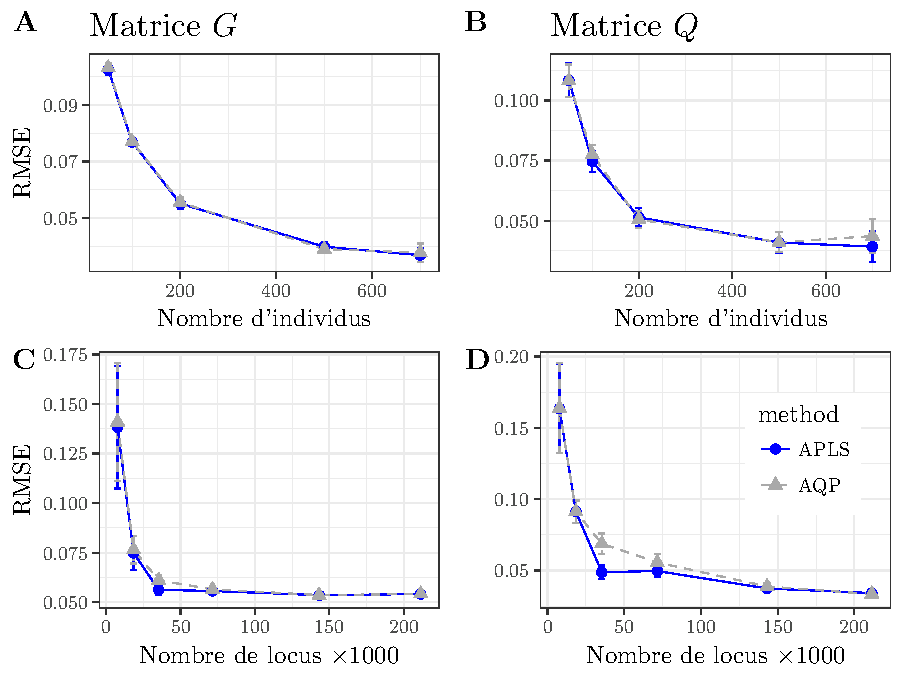
\includegraphics{./OUTPUT/Rplots/tess3_APLS_AQP_rmse_comp.pdf}
\caption{{\bf Racine carré de l'erreur quadratique moyenne (RMSE) pour les
    estimations des matrices $\Q$ et $\mathbf{G}$}. Simulations de génotype métissé
  spatialement. A-B) Erreur statistique des estimations de APLS et AQP en
  fonction du nombre d'individu $n$ ($p \sim 10^4$). C-D) Erreur statistique des
  estimations de APLS et AQP en fonction du nombre de locus $p$ ($n = 200$)}
\label{fig:tess3:comp}
\end{figure}

Nous avons sous-échantillonné un grand jeu de données de SNPs d'écotypes de
\emph{A.thaliana} pour comparer les propriétés de convergence et les temps
d'exécution des algorithmes AQP et APLS. Dans ces expériences, nous utilisons
les méthodes avec \(6\) clusters génétiques et avons répliqué 5 fois chaque
simulation. Pour un nombre d'individus allant de 500 à 600 et un nombre de 50k
locus, l'algorithme APLS nécessite plus d'itérations (25 itérations) que
l'algorithme AQP (20 itérations) pour converger vers sa solution (Figure
\ref{fig:tess3:vitesse}). Pour un nombre de locus allant de 10k à 200k et 150
individus, nous observons des résultats similaires. Pour 50k SNPs, les temps
d'exécution sont significativement plus bas pour l'algorithme APLS que pour
l'algorithme AQP. Pour 50k SNPs et 600 individus, cela prend en moyenne 1,0 min
pour l'algorithme APLS et 100 min pour l'algorithme AQP pour calculer leurs
résultats. Pour 100k SNPs et 150 individus, il faut en moyenne 0,6 min (9,0 min)
pour l'algorithme APLS (AQP) pour calculer leurs résultats. Pour le spectre de
valeurs du nombre d'individus et de locus considéré, l'implémentation de
l'algorithme APLS est environ 2 à 100 fois plus rapide que celle de
l'algorithme AQP.

\begin{figure}[!t]
\centering
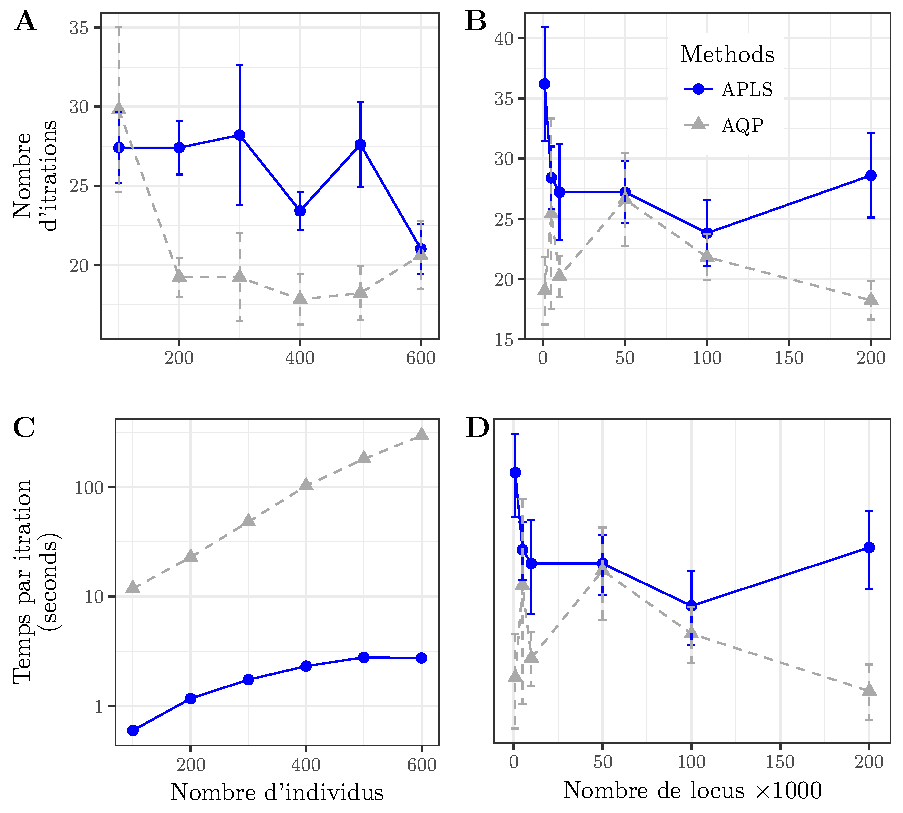
\includegraphics{./OUTPUT/Rplots/tess3_vitesse.pdf}
\caption{{\bf Nombre d'itérations et temps d'exécution pour les algorithmes AQP et
  APLS}. A-B) Nombre total d'itération avant que l'algorithmes ait atteint une
  solution stable. C-D) Temps de calcul d'une seul itération en secondes. Le
  nombre de SNPs a été fixé à $p = 50$k pour A et C. Le nombre d'individus a été
  fixé à $n = 150$ pour B et D.}
\label{fig:tess3:vitesse}
\end{figure}
\subsection{Comparaison avec une méthode spatiale bayésienne : TESS}
\label{sec:orga542833}

Nous avons utilisé des simulations coalescentes de polymorphismes neutres avec
un modèle spatial de mélange pour évaluer les capacités de l'algorithme APLS à
reproduire les estimations obtenues avec le logiciel \texttt{TESS} 2.3. Nous avons
simulé deux clusters génétiques de 100 échantillons de 2000 locus pour différent
niveau de différenciation moyen \(F_{\rm ST}\). Cela a permis de créer des jeux de
données pour lesquels il est plus ou moins difficile d'estimer la structure de
population. Les erreurs statistiques, mesurées par RMSE, pour l'estimation des
matrices \(\Q\) et \(\mathbf{G}\) varie entre \(0.02\) et \(0.15\) (Figure
\ref{fig:tess3:tess23}). Les erreurs statistiques augmentent à mesure que les
niveaux de différenciation entre les deux populations sources diminuent, mais
elles reste dans une gamme acceptable pour les valeurs de \(F_{\rm ST} > 0.016\).
Dans l'ensemble, les performances statistiques sont du même ordre pour \texttt{TESS}
2.3 et APLS.

\begin{figure}[!t]
\centering
\begin{minipage}{0.49\textwidth}
  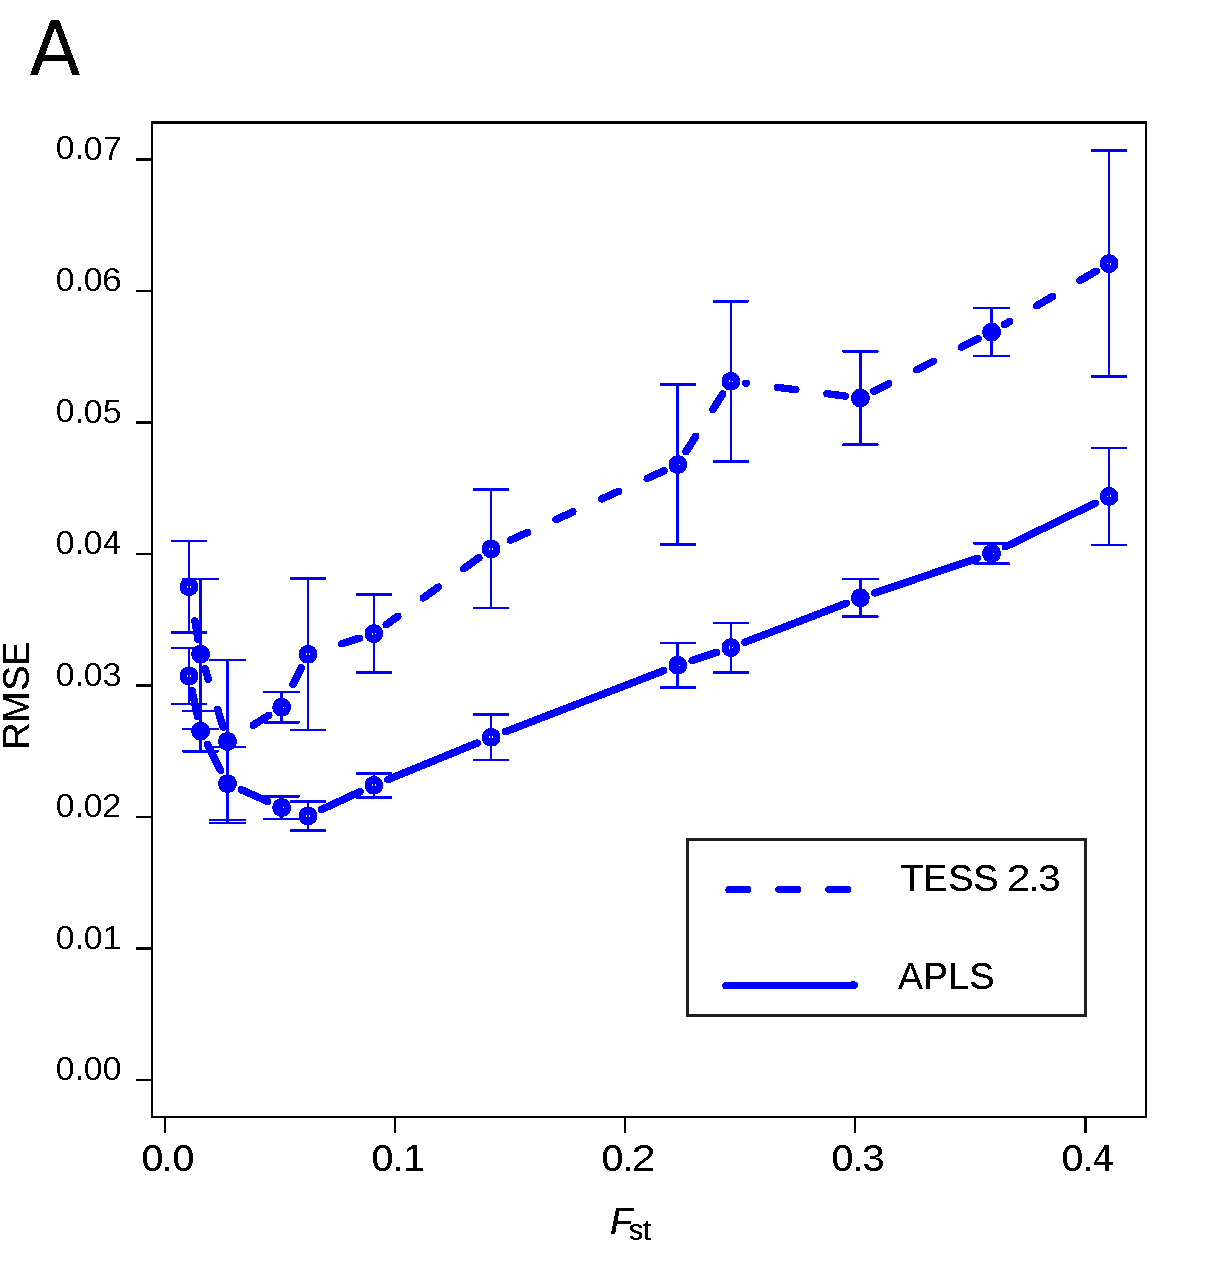
\includegraphics[width=\textwidth]{./OUTPUT/Rplots/tess3_tess2_3_rmseG.pdf}
\end{minipage}
\begin {minipage}{0.49\textwidth}
  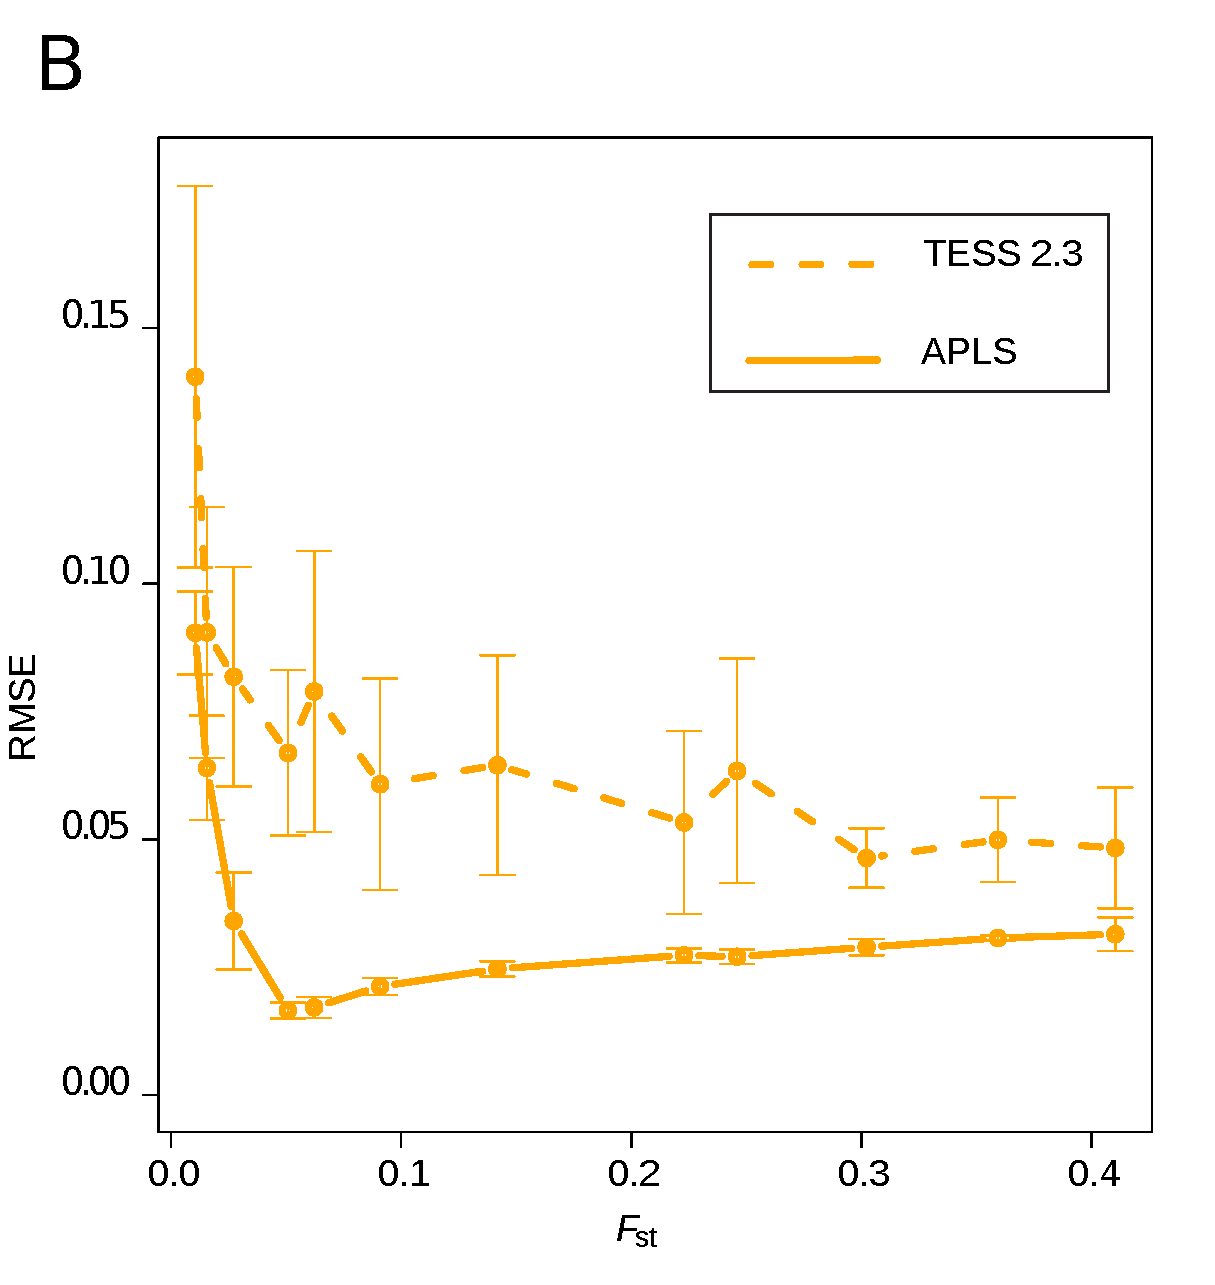
\includegraphics[width=\textwidth]{./OUTPUT/Rplots/tess3_tess2_3_rmseQ.pdf}
\end{minipage}
\caption{{\bf Racine de l'erreur quadratique moyenne (RMSE) pour l'estimation de
    $\Q$ (figure A) et $\mathbf{G}$ (figure B).} Simulations de génotypes métissés
  spatialement pour plusieurs niveaux de différenciation ($\Fst$) entre les
  populations sources. Les populations sources sont simulées par un modèle de
  Wright à deux îles et la statistique de différenciation est définie comme
  $1/(1+4N_0 m)$ où $m$ est le taux de migration et $N_0$ la taille
  effective de la population. Les erreurs statistiques de \textit{TESS} 2.3 et APLS sont
  représentées comme des fonctions de $\Fst$.}
\label{fig:tess3:tess23}
\end{figure}    
\subsection{Comparaison avec une méthode non spatiale : sNMF}
\label{sec:org2d40b31}

En utilisant des simulations coalescentes de polymorphismes neutres avec un
modèle spatial de mélange, nous avons comparé les estimations statistiques
obtenues à partir d'un algorithme spatial (APLS) et d'un algorithme non spatial
(sNMF, \cite{Frichot_2014}). Pour différents niveaux de différenciation de la
population ancestrale, les estimations obtenues à partir de l'algorithme spatial
sont plus précises que celles obtenues en utilisant des approches non spatiales
(Figure \ref{fig:tess3:comp:rmse:snmf}). Pour les données simulées plus grandes,
la méthode spatiale arrive à détecter une structure de population plus fine que
l'algorithme non spatial (Figure \ref{fig:tess3:comp:rmse:snmf}).

\begin{figure}[!t]
\centering
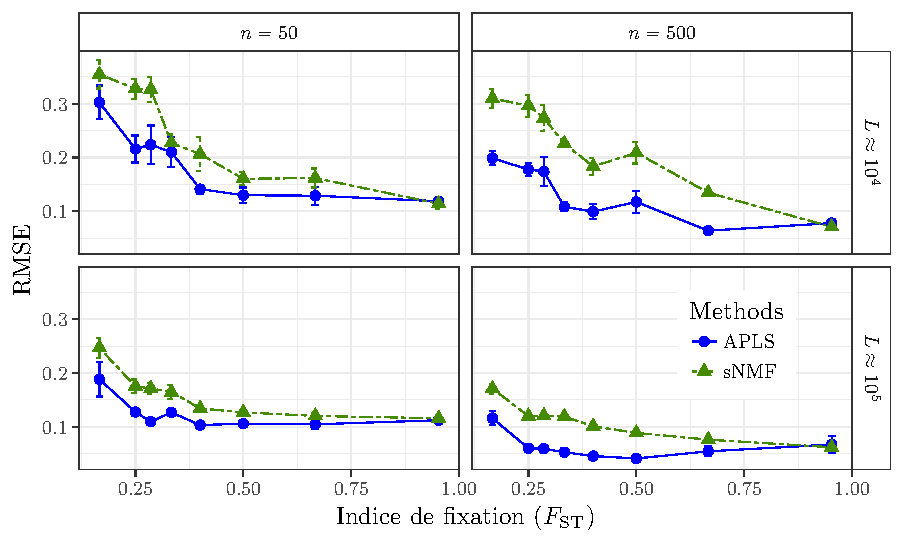
\includegraphics{./OUTPUT/Rplots/tess3_comp_rmse_snmf.pdf}
\caption{{\bf Racine de l'erreur quadratique moyenne (RMSE) pour l'estimation de
    $\Q$.} Simulations de génotypes métissés spatialement pour plusieurs niveaux
  de différenciation($F_{\rm ST}$) entre les populations sources. Les
  populations sources sont simulées par un modèle de Wright à deux îles et la
  statistique de différenciation est définie comme $1 / (1 + 4 N_0 m)$ où $m$
  est le taux de migration et $N_0$ la taille effective de la population. Les
  erreurs statistiques de sNMF et APLS sont représentées comme des fonctions de
  $F_{\rm ST}$.}
\label{fig:tess3:comp:rmse:snmf}
\end{figure}

Sur les simulations avec des locus sous adaptation locale, nous avons utilisé
l'aire sous la courbe de précision-rappel (AUC) pour quantifier les performances
des tests de détection des locus sélectionnés reposant sur les estimations des
matrices d'ascendance génétique, \(\Q\) et \(\mathbf{G}\). De plus, nous avons
calculé les AUC pour des tests de neutralité basés sur le calcul de la \(\Fst\) à
partir des génotypes des populations sources avant le mélange. Comme ils
représentent les valeurs maximales atteignables, les AUC basés sur les génotypes
des populations sources sont toujours plus élevés que ceux obtenus pour des
tests basés sur des estimations des matrices d'ascendance. Pour toutes les
valeurs de l'intensité de sélection (le rapport des taux de migration aux locus
neutres et adaptatifs), les AUC sont plus élevées pour les méthodes spatiales
que pour les méthodes non spatiales (Figure \ref{fig:tess3:auc}). Pour les
intensités de sélection élevées, les performances des tests fondés sur les
estimations des matrices d'ascendance sont proches des valeurs optimales
atteintes par des tests basés sur les fréquences dans les populations sources
simulées par \texttt{ms}. Ces résultats fournissent des preuves que l'inclusion de
l'information spatiale dans les algorithmes d'estimation de l'ascendance
améliore la détection des signatures de balayage sélectif survenant dans des
clusters génétiques inconnus.

\begin{figure}[!t]
\centering
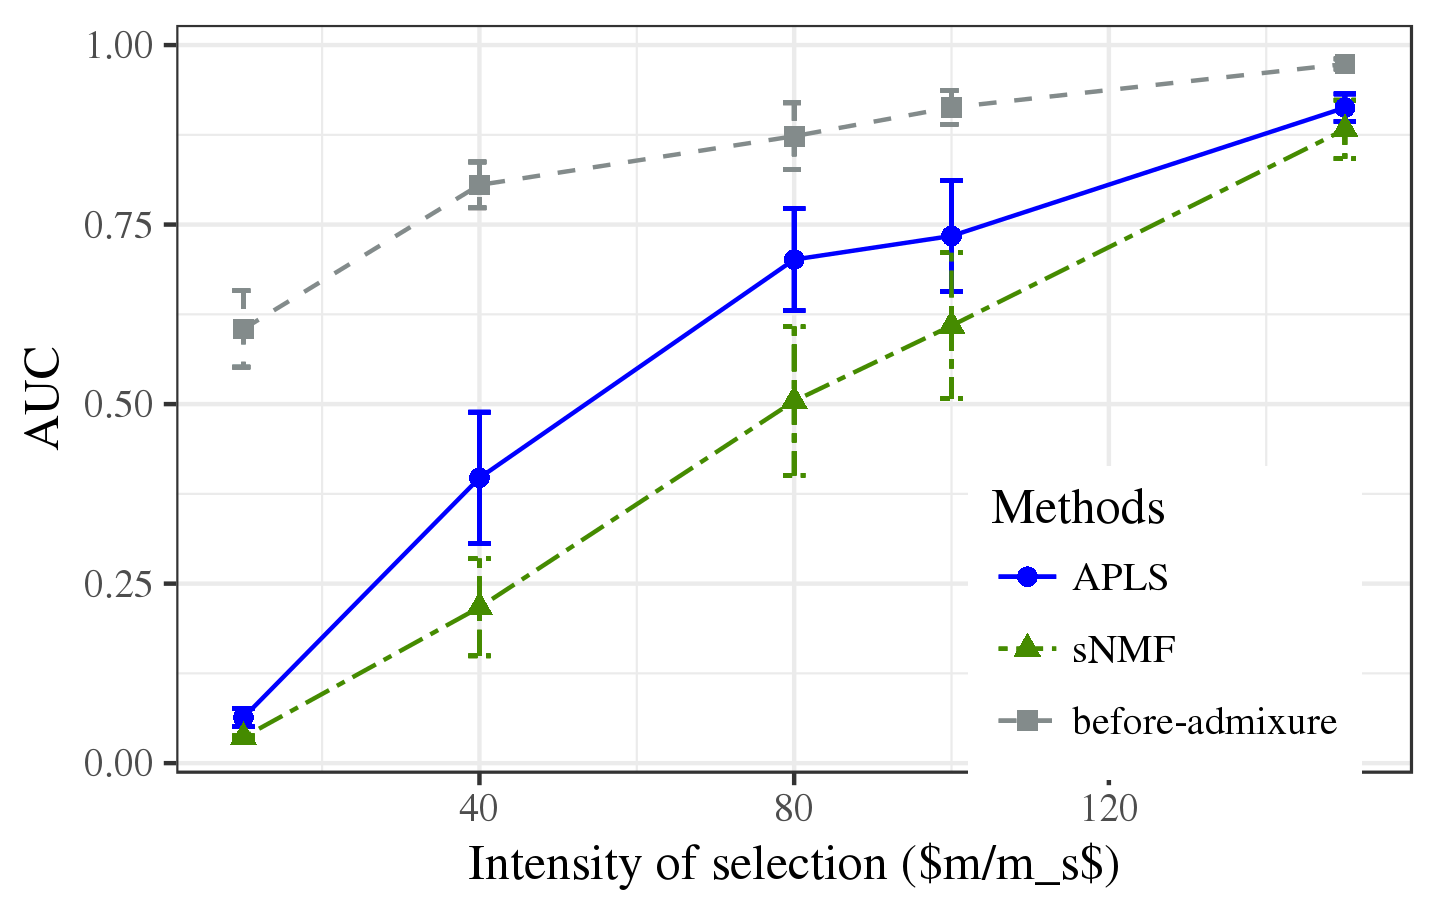
\includegraphics{./OUTPUT/Rplots/tess3_comp_auc_snmf.pdf}
\caption{{\bf Aire sous la courbe de précision-rappel (AUC).} Tests de
  neutralité appliqués aux simulations de populations spatialement métissées.
  Nous avons calculé l'AUC pour les tests basés sur la statistique $F_{\rm ST}$
  calculée à partir des vrais populations sources avant le métissage, à partir
  des estimations d'ascendance spatiale calculées avec l'algorithme APLS,
  l'estimations d'ascendance non spatiales ({\tt structure}) calculées avec
  l'algorithme {\ tt snmf}. L'intensité de la sélection dans les populations
  sources, définies comme le rapport $ m / m_s $, varie dans la fourchette
  de $1-160$.}
\label{fig:tess3:auc}
\end{figure}
\subsection{Sensibilité des estimateurs aux erreurs dans les mesures spatiales}
\label{sec:org9d81990}
Ensuite, nous avons utilisé les jeux de données simulées afin d'évaluer la
robustesse des estimations APLS pour des mesures inexactes des coordonnées
spatiales. À cette fin, un bruit gaussien a été ajouté aux coordonnées
géographiques vraiment observées en considérant les valeurs du rapport signal
sur bruit allant de 0 à 3. Nous avons calculé le variogramme spatial pour toutes
les simulations et avons constaté que la corrélation entre les données
génétiques et spatiales disparaît complétement pour un niveau de signal sur
bruit valant 2. Pour toutes les simulations, nous avons comparé l'erreur des
estimations de la matrice \(\Q\) fournies par APLS, relativement à celle obtenue
par la méthode non spatiale sNMF. Pour de faibles niveaux d'incertitude dans les
coordonnées spatiales, les erreurs statistiques des estimations APLS sont
inférieures à celles de sNMF (Figure \ref{fig:tess3:noise}). Pour les simulations
avec \(n = 500\) individus et \(p = 10^{5}\) locus, un rapport de signal sur bruit
important augmente les erreurs statistiques dans les estimations de la matrice
\(\Q\) de l'algorithme APLS. Pour un rapport signal sur bruit plus petit, les RMSE
sont généralement inférieurs pour l'algorithme APLS que pour la méthode sans
coordonnées spatiales. Pour les simulations avec \(n = 50\) individus et \(p =
10^4\) locus, les estimations APLS étaient plus précises que les estimations non
spatiales. Ce résultat inattendu s'explique par des différences algorithmiques
subtiles dans les programmes testés. Dans une large mesure, les estimations de
l'algorithme APLS sont robustes à l'incertitude dans les mesures spatiales. Des
tests graphiques standards tels qu'une analyse de variogramme peuvent aider à
décider si notre algorithme spatialement explicite est utile ou non.

\begin{figure}[!t]
\centering
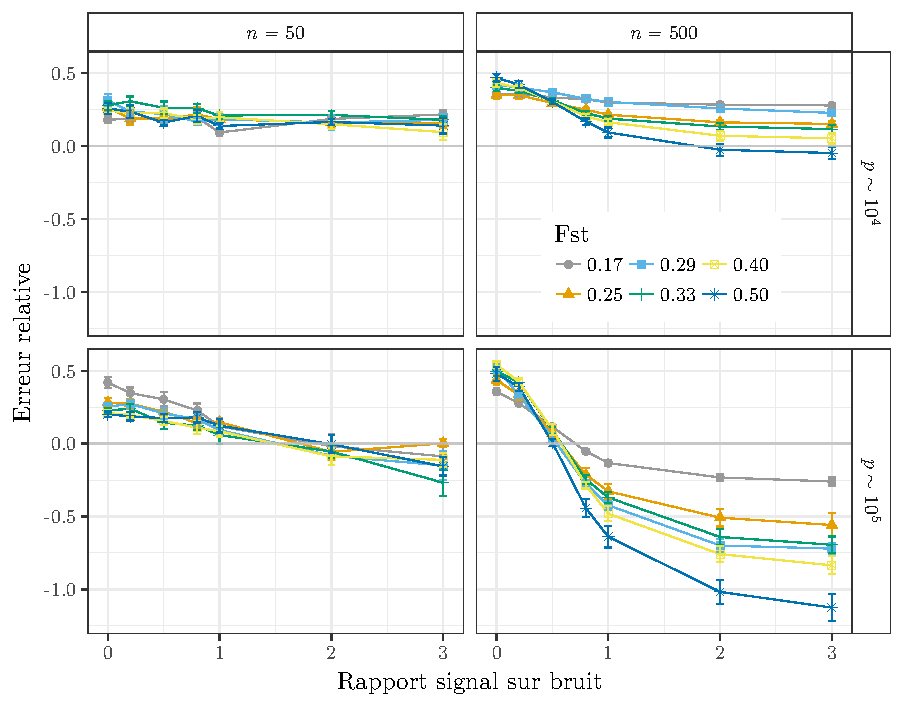
\includegraphics{./OUTPUT/Rplots/tess3_noise.pdf}
\caption{{\bf Impact de l'incertitude dans les coordonnées géographiques sur les
    estimations des coefficients de métissage.} Erreur statistique relative des
  estimations des coefficients de métissage obtenues à partir de l'algorithme
  APLS pour plusieurs niveaux du rapport bruit-signal et des valeurs de l'indice
  de fixation ($\Fst$). La méthode sNMF a été considéré comme la référence pour
  la méthode non spatiale (valeur 0)}
\label{fig:tess3:noise}
\end{figure}

\subsection{Application à des données Arabidopsis Thaliana}
\label{sec:orgacbd936}

Nous avons utilisé l'algorithme APLS pour étudier la structure génétique de
population spatiale et effectuer un balayage du génome pour les allèles
adaptatifs dans des écotypes européens de l'espèce végétale \emph{A. thaliana}. Le
critère de validation croisée diminue rapidement pour \(K = 1\) à \(K = 3\) nombre
de clusters, indiquant qu'il y a trois clusters génétiques principaux en Europe,
correspondant aux régions géographiques d'Europe occidentale, d'Europe centrale
et orientale et de Scandinavie septentrionale. Pour un nombre de clusters \(K\)
supérieur à 4, les valeurs du critère de validation croisée diminue de
manière plus lente; ce qui indique qu'une sous-structure subtile, résultant de
processus historiques complexes d'isolement par distance, pourrait également être
détectée (Figure \ref{fig:tess3:at:param}). Le variogramme spatial donne une
echelle spatiale approximative de \(\sigma = 150\) km (Figure
\ref{fig:tess3:at:param}). La figure \ref{fig:tess3:at:map} affiche l'estimation de
la matrice \(\Q\) interpolée sur une carte géographique d'Europe pour 6 clusters
génétiques. L'estimation des coefficients de métissage fournit une preuve
claire du regroupement des écotypes dans des groupes génétiques spatialement
homogènes.

\begin{figure}[!t]
\centering
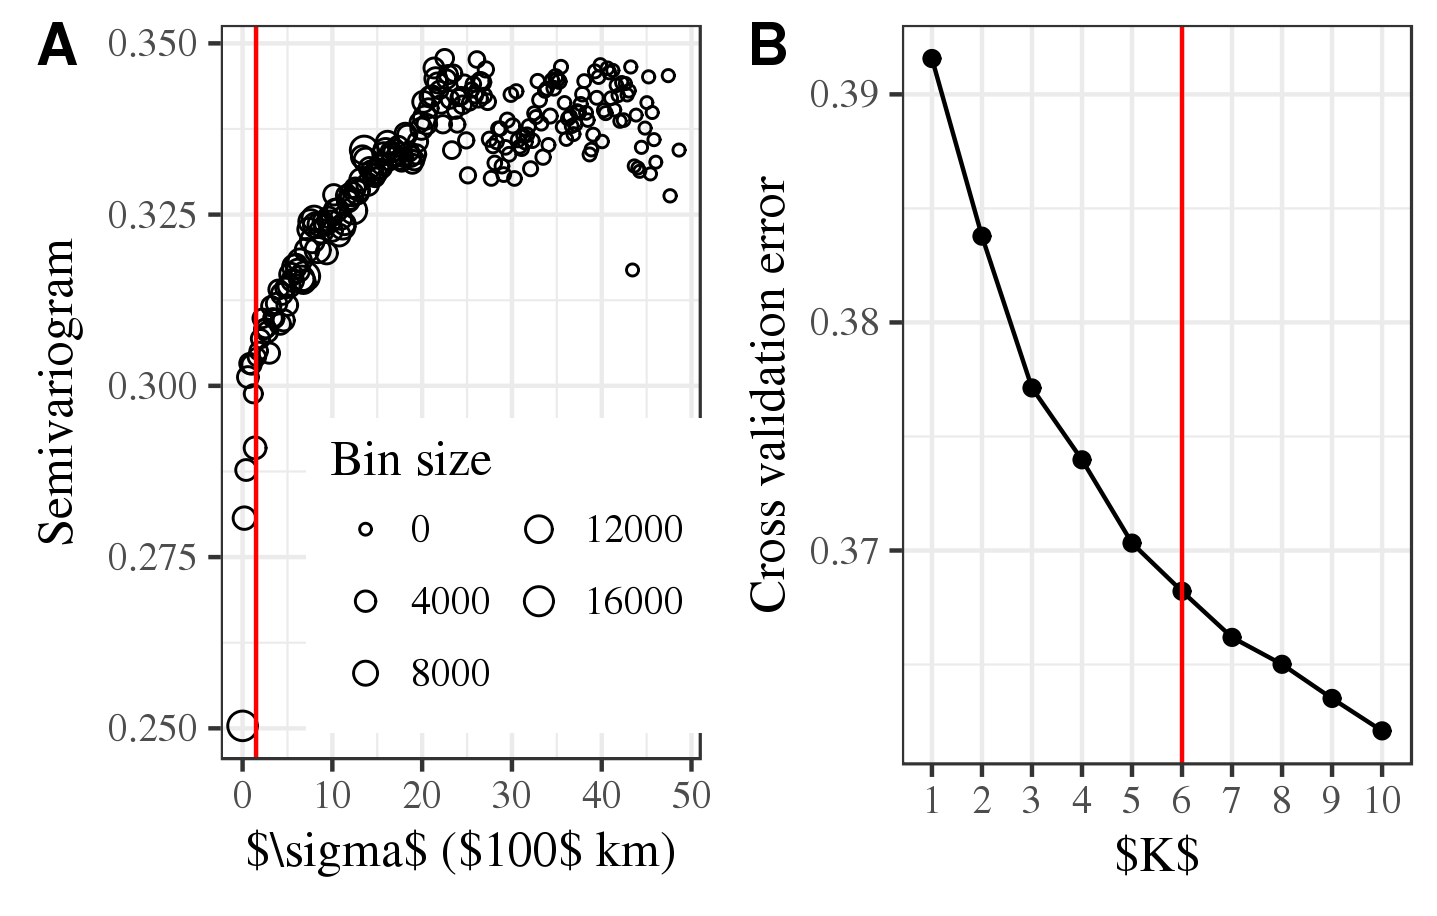
\includegraphics{./OUTPUT/Rplots/tess3_AT_params.pdf}
\caption{{\bf Choix de $\sigma$ et $K$ pour l'algorithme APLS}. A) Variogramme
  empirique pour les données {\it A. thaliana}. La ligne verticale rouge montre
  la valeur de l'échelle géographique choisie, $\sigma = 1.5$. B) Erreur de
  validation croisée en fonction du nombre de clusters génétiques, $K$. La
  ligne verticale rouge montre le nombre de clusters génétiques choisi, $K=6$.}
\label{fig:tess3:at:param}
\end{figure}

\begin{sidewaysfigure}[!t]
\centering
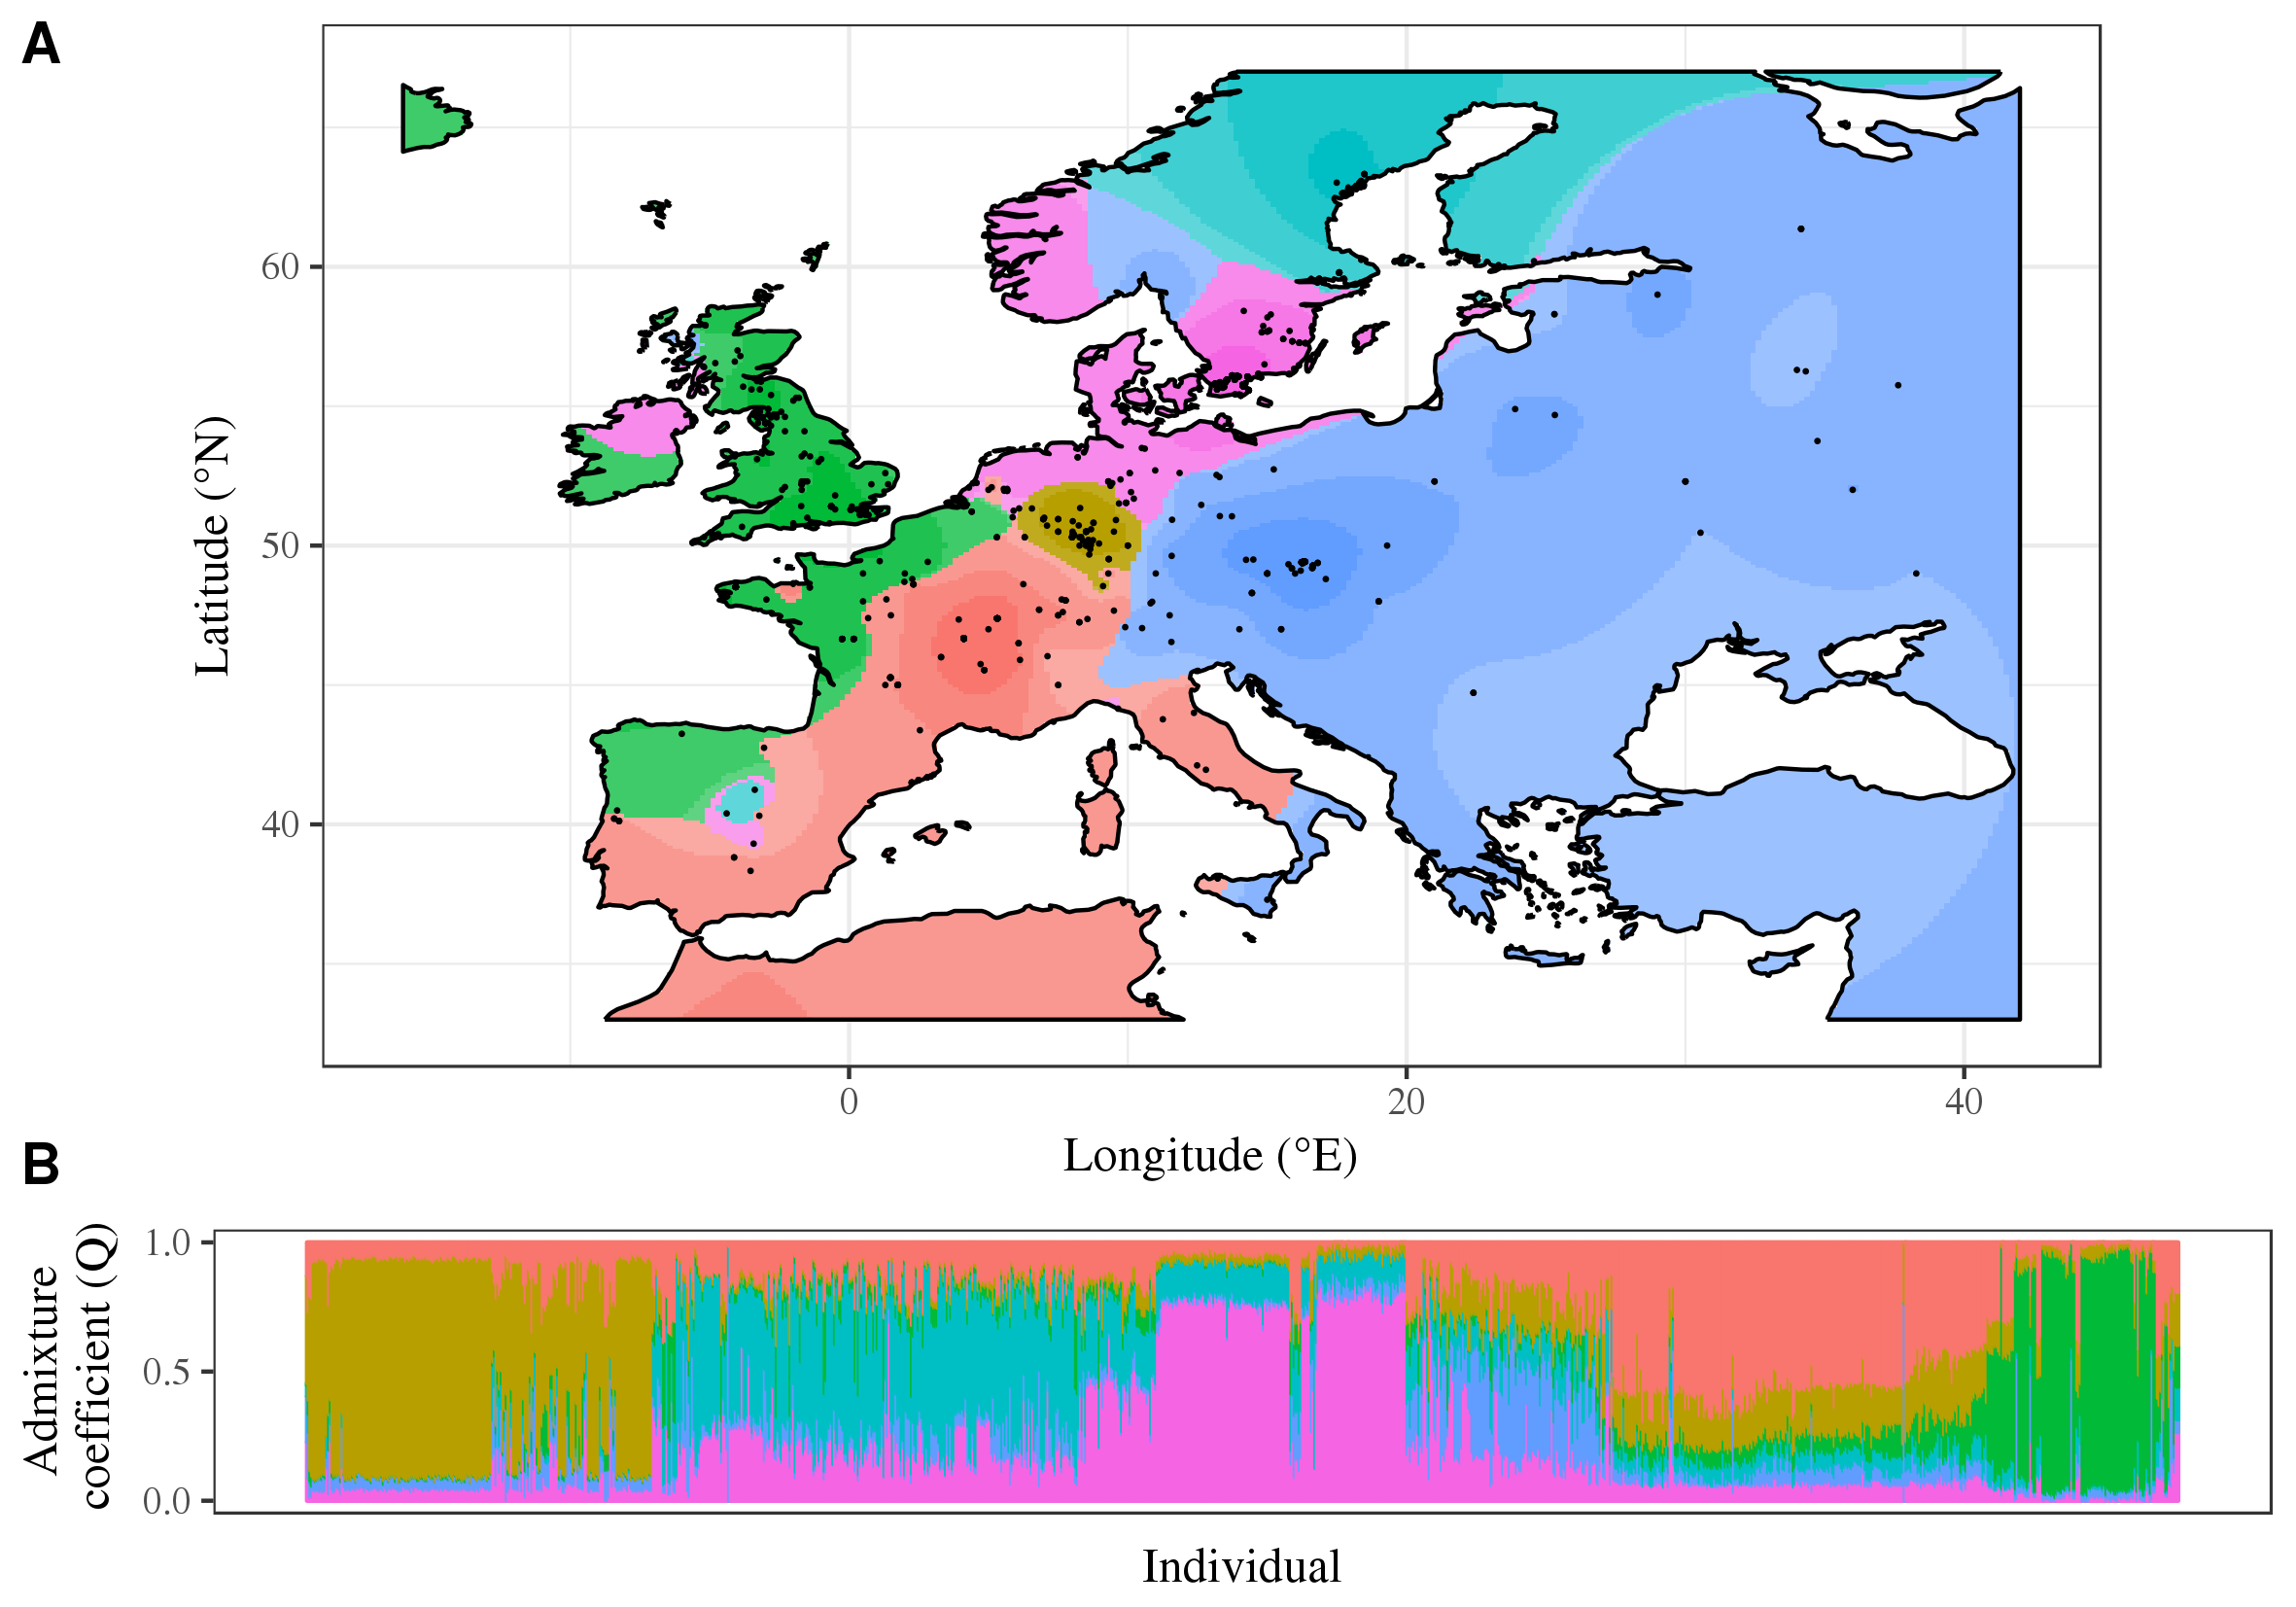
\includegraphics{./OUTPUT/Rplots/tess3_AT_map.pdf}
\caption{{\bf {\it A. thaliana} coefficients de métissage}. Estimation des
  coefficients de métissage calculée par l'algorithme APLS avec $K = 6$ clusters
  génétiques et $\sigma = 1.5$ pour le paramètre d'échelle géographique. A)
  Carte géographique des coefficients de métissage. B) Barplot des coefficients
  de métissage.}
\label{fig:tess3:at:map}
\end{sidewaysfigure}

Les tests basés sur la statistique \(\Fst\) ont été appliqués à l'ensemble de 214k
SNP pour détecter les locus sous sélection naturelle dans le génome de l'espèce
\emph{A.thaliana}. \emph{A. thaliana} se trouve dans une large variété d'habitats, et
l'adaptation locale à l'environnement est reconnue comme étant une pression
importante qui façonne la diversité génétique dans l'espace
\citep{Hancock2011,Fournier-Level2011}. L'algorithme APLS a été exécuté sur les
1095 écotypes européennes de \emph{A. thaliana} avec 6 clusters génétiques et 1.5
pour le paramètre d'échelle spatiale. En utilisant l'algorithme
Benjamini-Hochberg pour contrôler le FDR à \(1 \%\), le programme a produit une
liste de 12 701 SNPs candidats. Les 100 meilleurs candidats incluent des SNPs
dans les gènes liés à la floraison SHORT VEGETATIVE PHASE (SVP),
COP1-interacting protein 4.1 (CIP4.1) et FRIGIDA (FRI) (\(p\text{-valeur} <
10^{-300}\)). Ces gènes ont été détectés par des analyses antérieures de la
sélection sur cet ensemble de données \citep{Horton_2012}. Nous avons réalisé une
analyse d'enrichissement en ontologie des gènes en utilisant AmiGO afin
d'évaluer quelles fonctions biologiques pourraient être impliquées dans
l'adaptation locale en Europe. Nous avons trouvé une sur-représentation
significative des gènes impliqués dans les processus cellulaires (\(1.06\) fois
plus que l'attendu, et une \pvalue égale à \(0.0215\) après correction de
Bonferonni).

\begin{sidewaysfigure}[!t]
\centering
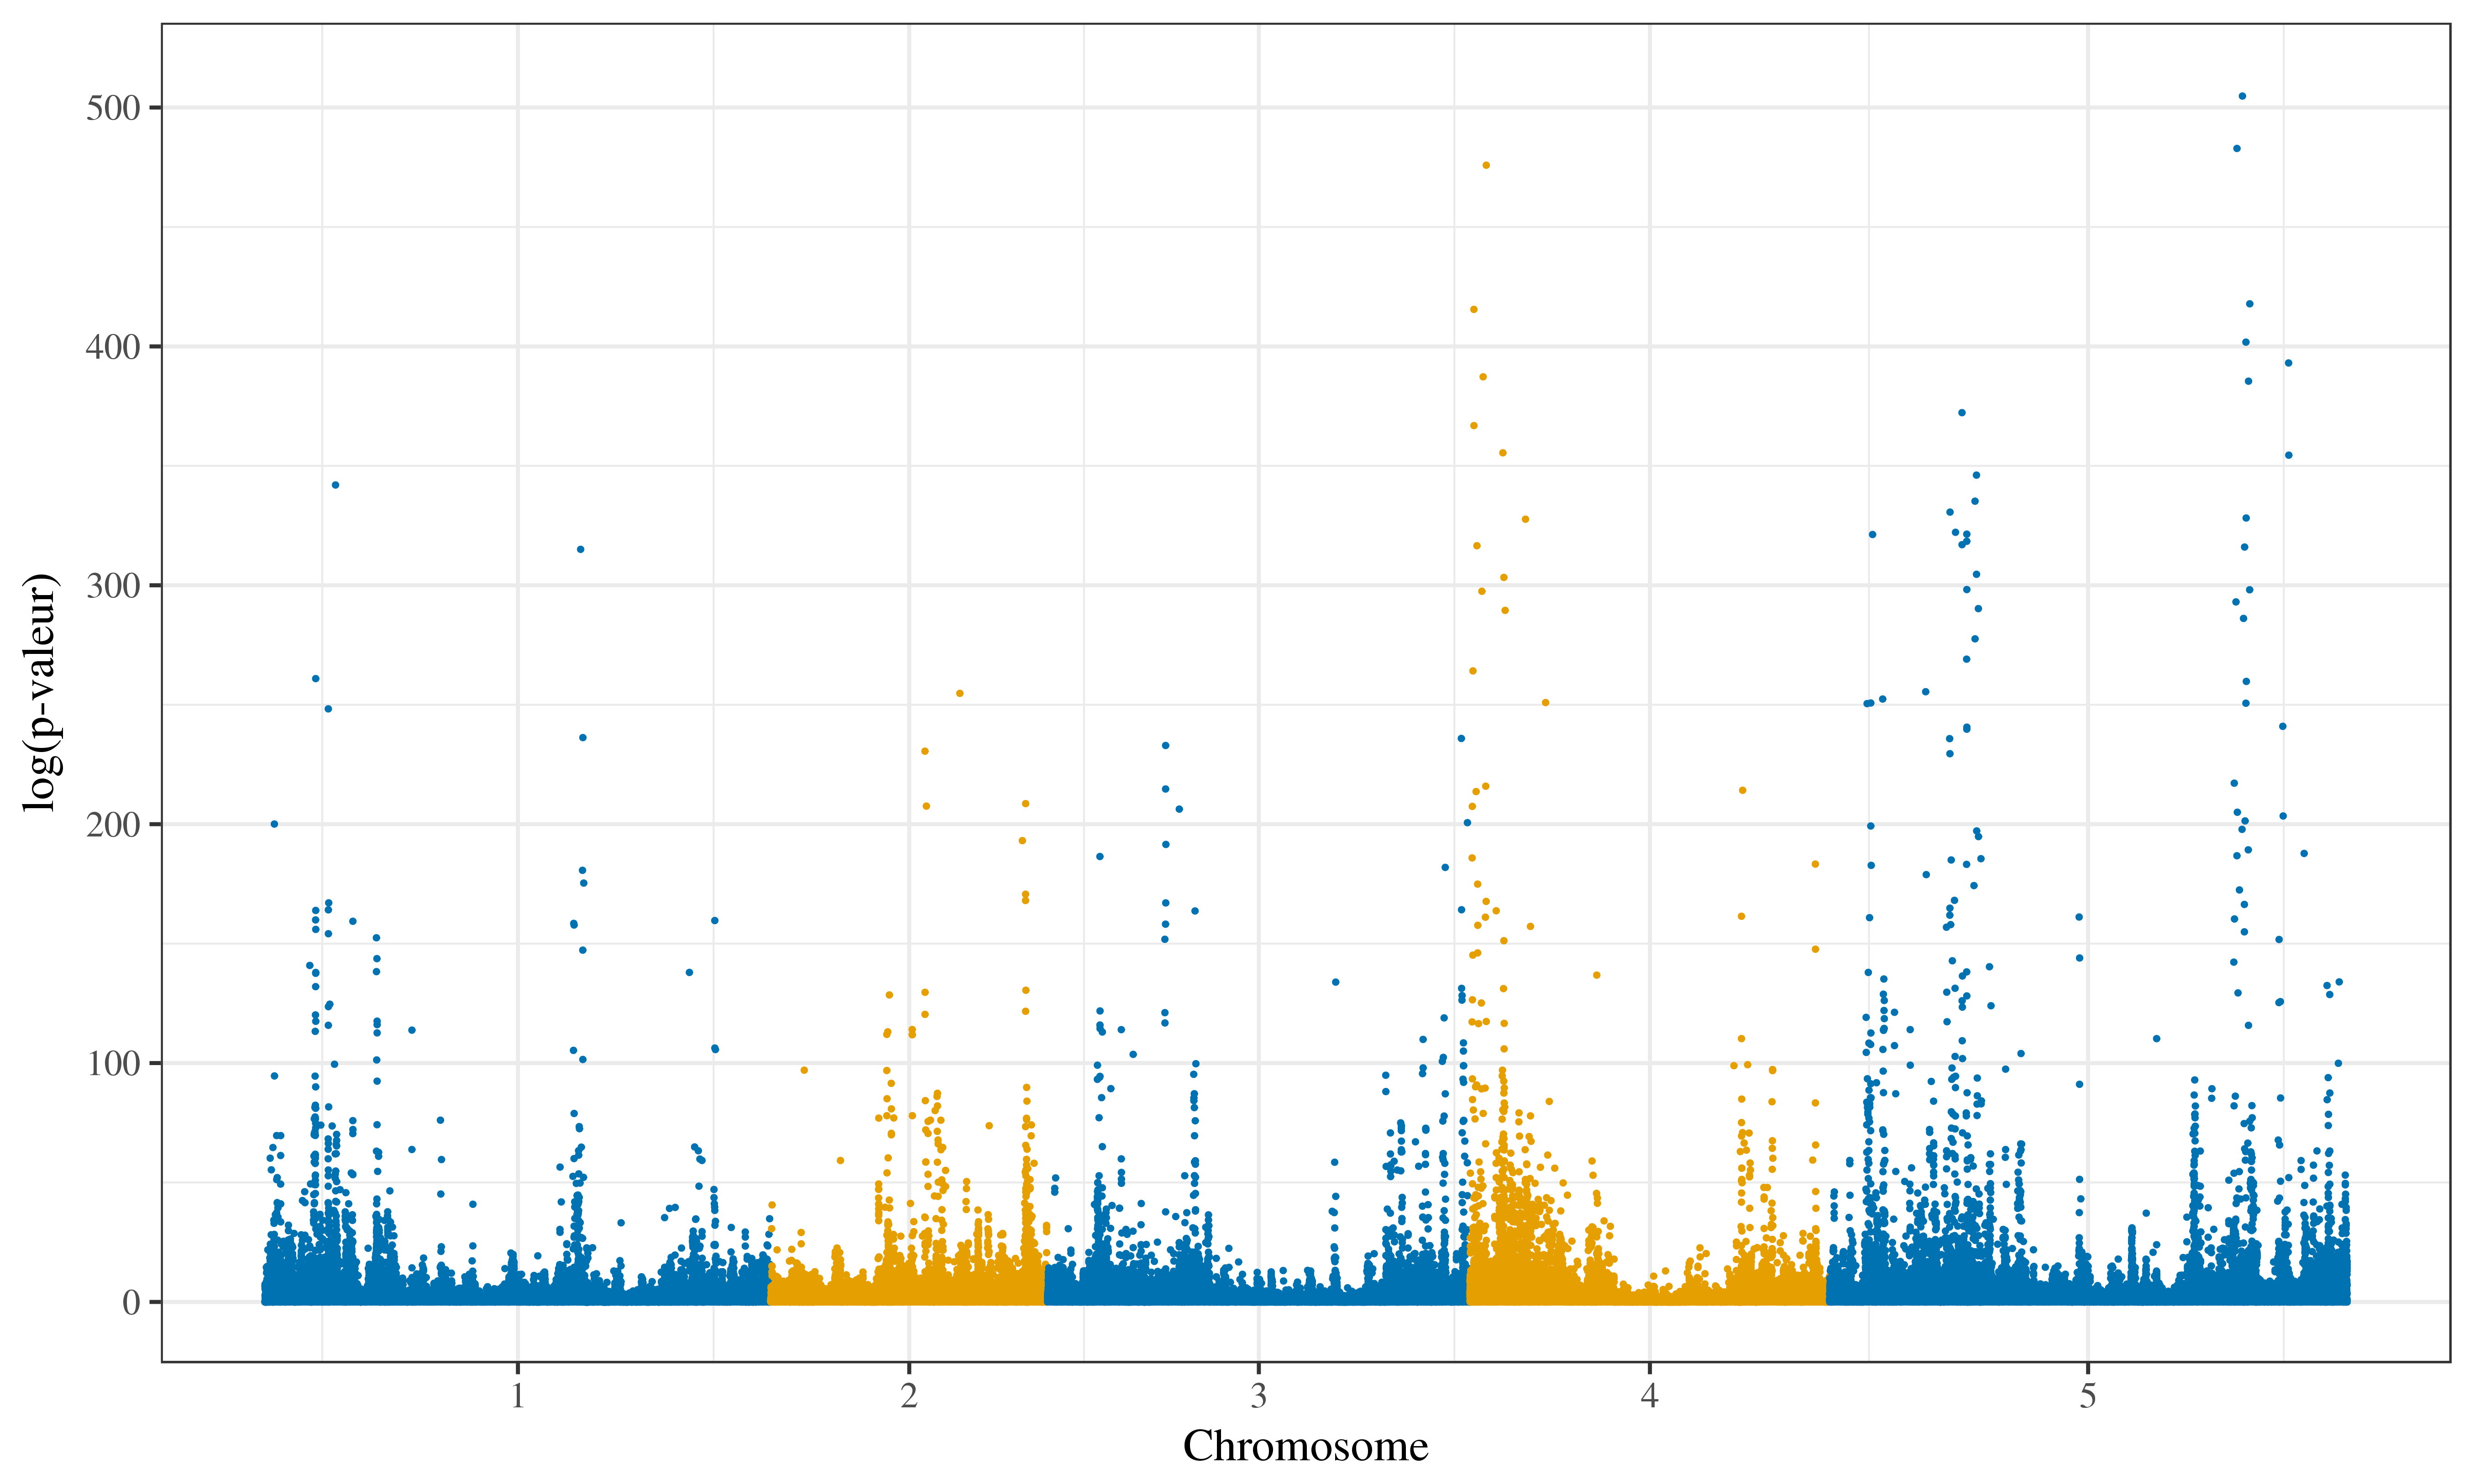
\includegraphics{./OUTPUT/Rplots/tess3_AT_manhattanplot.png}
\caption{{\bf Détection de locus sous adaptation locale sur des écotypes
    européennes de \bf {\it A. thaliana}}. Manhattan plot de
  $-\log(p\text{-value})$. Les \pvalues ont été calculées à partir de la
  structure de la population estimée par l'algorithme APLS avec $K = 6$ clusters
  génétiques et $ \sigma = 1,5 $ pour le paramètre d'échelle géographique.}
\label{fig:tess3:at:manhattanplot}
\end{sidewaysfigure}

\section{Discussion}
\label{sec:org7254bca}
L'inclusion de l'information géographique dans l'inférence des relations
ancestrales entre les organismes est un objectif majeur des études en génétique
des populations \citep{Malecot1948,Epperson_1996,Cavalli-Sforza1994}. En supposant
que des individus géographiquement proches sont plus susceptibles de partager la
même ascendance que des individus dans des sites éloignés, nous avons introduit
deux nouveaux algorithmes pour estimer les proportions d'ascendance à l'aide
d'informations géographiques et génétiques. Sur la base des problèmes de
moindres carrés, les nouveaux algorithmes combinent des approches de
factorisation matricielle et de statistiques spatiales pour fournir des
estimations précises des coefficients de métissage individuels et des fréquences
d'allèle dans les clusters génétiques. Les deux algorithmes partagent de nombreuses
similitudes, mais ils diffèrent dans les approximations qu'ils font pour
diminuer la complexité algorithmique. Plus précisément, l'algorithme AQP alterne
des résolutions de problèmes d'optimisation quadratique alors que l'algorithme
APLS lève les contraintes des problèmes d'optimisation afin de les transformer
en problèmes des moindres carrés. La complexité algorithmique de l'algorithme
APLS augmente linéairement avec le nombre d'individus dans l'échantillon en
ayant la même précision statistique que l'algorithme AQP plus lent.

Pour mesurer le bénéfice de l'utilisation d'algorithmes spatiaux, nous avons
comparé les erreurs statistiques observées pour les algorithmes spatiaux avec
celles observées pour les algorithmes non spatiaux. Dans nos expériences
numériques les erreurs des méthodes spatiales sont inférieures à celles
observées avec des méthodes non spatiales, et les algorithmes spatiaux ont
permis de détecter une structure de population plus subtile. En outre, nous
avons mis en place un test de détection de la sélection reposant sur les
estimations spatiales des matrices \(\Q\) et \(\mathbf{G}\) \citep{Martins_2016}; et
nous avons observé que les tests rejettent la neutralité des locus avec plus de
précision que ceux fondés sur des approches non spatiales. Ainsi, l'information
spatiale a contribué à améliorer la détection des signatures de balayage
sélectif survenant dans des populations sources avant les événements de mélange.
Nous avons appliqué les tests de neutralité afin d'effectuer un balayage du
génome pour la sélection dans des écotypes européens de l'espèce végétale
\emph{A.thaliana}. Le scan du génome a confirmé la preuve de la sélection des gènes
liés à la floraison \emph{CIP4.1}, \emph{FRI} et \emph{DOG1} différenciant la Fenno-Scandinavie
du nord-ouest de l'Europe \citep{Horton_2012}.

L'estimation des coefficients de métissage, en utilisant des algorithmes rapides
qui étendent des approches non spatiales telles que \texttt{structure}, a été
intensément discutée au cours des dernières années \citep{Wollstein2015}. Dans ces
améliorations, les approches spatiales ont reçu moins d'attention que les
approches non spatiales. Dans cette étude, nous avons présenté un cadre
conceptuelle permettant de développer des méthodes rapides d'estimation de
l'ascendance spatiale. Ces méthodes rapides sont implémentées dans le package
\texttt{tess3r} qui propose une pipeline intégrée pour l'estimation et la visualisation
de la structure génétique de population et pour la recherche de locus
responsables de l'adaptation locale. La complexité algorithmique de nos
algorithmes permet à leurs utilisateurs d'analyser des échantillons comprenant
des centaines à des milliers d'individus. Par exemple, l'analyse de plus d'un
millier de génotypes \emph{A.thaliana}, chacun incluant plus de 210k SNP, n'a pris
que quelques minutes à l'aide d'un seul CPU.

\chapter[Algorithmes d'estimation des facteurs de confusion]{Algorithmes d'estimation pour les modèles de régression à facteurs latents}
\label{sec:org64484ff}
\label{orga10073b}

\section{Résumé}
\label{sec:org0afad26}

Les études d'association sont massivement utilisées en biologie. Elles
permettent par exemple de découvrir les causes génétiques d'une maladie ou bien
les gènes impliqués dans un processus d'adaptation au climat. Lors de ces
études, nous sommes amenés à tester les corrélations entre un grand nombre de
variables, comme par exemple des SNPs, et une variable d'intérêt, comme par
exemple une maladie. Dans certaines de ces études, des sources de variation
indésirable, telles que la structure de populations, ou bien les conditions
expérimentales, peuvent sévèrement biaiser les résultats des tests. Une méthode
communément utilisée consiste à modéliser les sources de variation indésirable à
l'aide de variables latentes. Dans ce chapitre, nous introduisons deux nouveaux
algorithmes qui permettent d'estimer les variables latentes afin de corriger les
études d'association pour les sources de variation indésirable. Nous appelons
ces variables latentes les facteurs de confusion pour l'étude d'association.
Nous utilisons l'approche classique qui consiste à ajouter un terme factoriel au
modèle de régression des variables étudiées par des variables d'intérêts. Nos
deux algorithmes reposent sur différentes régularisations portant sur les effets
d'intérêt. Le premier algorithme utilise une régularisation en norme \(L_{2}\),
tandis que le second utilise un régularisation en norme \(L_{1}\). Pour chaque
algorithme, nous démontrons leur convergence vers le minimum de leur fonction
objectif respective. Nous montrons sur des simulations numériques que nos
algorithmes reproduisent les performances d'autres algorithmes de correction
pour les études d'association. Nous montrons enfin que nos algorithmes
permettent de reproduire des résultats d'une étude d'association entre des
variants génétiques humain et la maladie \celiac, ainsi qu'une étude
d'association entre des niveaux de méthylation de l'ADN et la polyarthrite
rhumatoïde. Nous présentons enfin des résultats trouvés par nos algorithmes sur
un exemple d'étude d'association entre des génotypes et un gradient climatique.
Nos algorithmes sont implémentés dans le package R, \texttt{lfmm}.

\section{Introduction}
\label{sec:org846b5e1}
\label{org9613dc6} 


Au cours de la dernière décennie, des études d'association à grande échelle ont
été utilisées pour identifier des gènes candidats associés à une maladie
particulière ou un trait phénotypique d'intérêt. Selon le type des marqueurs
moléculaires examinés dans les génomes ou dans les cellules, plusieurs
catégories d'étude d'association ont été menées pour détecter des corrélations
significatives entre les marqueurs et le phénotype. Par exemple, les études
d'association à l'échelle du génome (GWAS genome-wide association studies) se
concentrent sur des polymorphismes à un seul nucléotide (SNP pour
single-nucleotide polymorphism) en examinant des variants génétiques chez
différents individus \citep{Balding_2006}. Les GWAS ont été étendues à des études
d'association à l'échelle de l'épigénome (EWAS epigenome-wide association
studies) qui mesurent les niveaux de méthylation de l'ADN chez différents
individus pour des associations entre la variation épigénétique et des
phénotypes \citep{Rakyan_2011}. Des approches similaires ont été appliquées à la
caractérisation de la variation observée dans l'ARN par rapport à différents
environnements, traitements médicaux, phénotypes ou maladies \citep{Slonim_2002}.
D'autres exemples d'études d'association incluent des études d'association
génétique-environnement (GEAS) dans lesquelles des locus sont testés pour leurs
corrélations avec des gradients écologiques afin de détecter des signatures de
sélection naturelle \citep{rellstab15_pract_guide_to_envir_assoc}. En peu de
temps, les études d'association ont permis des progrès considérables dans
l'identification des variants génétiques, qui confèrent une susceptibilité aux
maladies, ainsi qu'une compréhension plus approfondie de l'évolution des génomes
en réponse à la sélection naturelle.

\subsection{Méthodes de correction pour les facteurs latents}
\label{sec:org8b965cd}
Dans cette section, nous nous plaçons dans le cadre méthodologique des modèles
de régression linéaire. Il s'agit d'un cadre très utilisé en étude d'association
que nous pouvons formaliser de la façon suivante
\begin{equation}
\label{eq:statReg}
\Y_{j} = \X b_{j} + \E_{j}
\end{equation}
où \(\Y_{j}\) est la matrice des observations de la variable d'indice \(j\) pour
\(\Yrow\) individus, typiquement constituée de variants génétiques. Le
coefficient \(b_{j}\) représente l'effet de la variable \(\X\) sur \(\Y_{j}\). La
matrice \(\E_{j}\) est la matrice de l'erreur résiduelle. Il arrive parfois que
l'on fasse la régression dans l'autre sens, la régression s'écrit alors
\begin{equation}
\label{eq:statRegRevers}
\X = \Y_{j} a_{j} + \E^{'}_{j},
\end{equation}
où \(\a_{j}\) représente l'effet de \(\Y_{j}\) sur \(\X\). Dans la suite nous
discutons de régression uniquement dans le sens de l'équation \eqref{eq:statReg}.
L'objectif est de trouver les coefficients \(b_{j}\) qui sont significativement
différents de zéro. Dans ce cas, nous disons que \(\Y_{j}\) est associée à \(\X\).
Comme nous l'avons évoqué dans la partie précédente, avec cette approche il est
possible qu'une ou plusieurs variables latentes soient corrélées à la fois à
\(\Y\) et à \(\X\). Dans ce cas, si nous ne considérons pas les variables latentes
comme variables explicatives de la régression, nous détectons un grand nombre de
variables \(\Y_{j}\) significativement corrélées à \(\X\). Nous allons
maintenant présenter différentes approches de correction des études
d'association pour les facteurs de confusion.

\subsubsection{Estimation des facteurs latents a priori}
\label{sec:org93f983a}
Une première approche consiste à estimer les variables latentes en faisant une
analyse factorielle de \(\Y\). On fait l'analyse factorielle a priori et sans
prendre en compte la variable \(\X\). Les variables latentes sont ensuite ajoutées
au modèle de régression avec les autres variables explicatives, de sorte que
nous avons
\begin{equation}
\Y_{j} = \X b_{j} + \bar{\matr{U}} \V_{j}^{T} + \E_{j}
\end{equation}
où \(\bare{\matr{U}}\) est la matrice des variables latentes calculée a priori et
\(\V_{j}\) la matrice des effets des variables latentes sur \(\Y_{j}\). Par exemple,
les méthodes EIGENSTRAT et Refactor calculent les variables latentes à l'aide de
l'analyse en composantes principales (ACP) de la matrice \(\Y\)
\citep{Price_2006,Rahmani_2016}.
\subsubsection{Les modèles mixtes}
\label{sec:org9186b3d}
Une autre approche de correction pour les facteurs de confusion est le modèle
mixte. Dans un tel modèle, on ajoute un effet aléatoire au modèle de la
régression
\begin{equation}
\label{eq:mixemodel}
\Y_{j} = \X \B^{T} + \matr{Z} \matr{\Gamma}_{j} + \E_{j},
\end{equation}
où \(\matr{Z}\) est une matrice fixée à l'avance ("design matrix" en anglais) et
\(\matr{\Gamma}_{j}\) est la matrice des effets aléatoires à estimer. Dans les
modèles mixtes, on suppose de plus que la matrice de covariance de l'effet
aléatoire est connue. La matrice de covariance doit correspondre à la variance
du facteur de confusion; elle est en général calculée à partir de \(\Y\). Les
modèles mixtes ont été largement utilisés pour les GWAS
\citep{Kang_2008,Zhou_2014}. Dans les GWAS, les rôles de \(\Y_{j}\) (un variant
génétique) et \(\X\) (un phénotype) sont inversés dans l'équation
\eqref{eq:mixemodel}; et l'effet aléatoire permet d'expliquer la variation de
\(\Y_{j}\) qui est due à la structure de population. Dans ce cas, la matrice de
covariance est estimée a priori à partir les données génétiques.
\subsubsection{Les modèles mixtes à facteurs latents (LFMM latent factor mixed model)}
\label{sec:org2e7b6bc}
Nous introduisons maintenant les modèles mixtes à facteurs latents. Pour de tels
modèles, l'équation de régression peut s'écrire comme ceci :
\begin{equation}
\label{eq:glfmm}
\Y = \X \B^{T} + \matr{U} \V^{T} + \E,
\end{equation}
Dans cette équation \(\matr{U}\) est la matrice des variables latentes et \(\V\) est
la matrice des effets des facteurs latents. La différence majeure entre LFMM et
les autres modèles est que l'on ne suppose rien a priori sur les facteurs de
confusion. Dans LFMM, l'estimation des variables latentes \(\matr{U}\) et des
effets de la variable explicative \(\B\) se font en même temps. Les matrices
\(\matr{U}\) et \(\V\) permettent d'apprendre les variations systématiques observées
dans la matrice \(\Y\) tandis que la matrice des effets \(\B\) permet d'apprendre
l'effet de \(\X\) sur les colonnes de \(\Y\). Il existe différentes méthodes pour
estimer les paramètres de LFMM. On distingue d'abord des approches qui reposent
sur des algorithmes de Monte-Carlo
\citep{Frichot_2013,carvalho08_high_dimen_spars_factor_model}. Ces approches
reposent sur une modélisation bayésienne qui permet d'échantillonner les lois a
posteriori des paramètres. L'avantage des méthodes MCMC est qu'elles permettent
d'estimer la variance du paramètre \(\B\) grâce au bootstrap bayésien
\citep{rubin1981bayesian}, et de faire un test de significativité statistique.
Certaines approches reposent sur des algorithmes EM (Expectation Maximisation)
\citep{friguet09_factor_model_approac_to_multip,agarwal09_regres,zhou16_spars_multiv_factor_analy_regres}.
Ces approches sont souvent plus rapides que les méthodes utilisant des
algorithmes de Monte-Carlo. Enfin, d'autres approches reposent sur une
estimation des variables latentes à partir d'une transformation de \(\Y\)
\citep{gerard2017unifying,wang2015confounder,article_Leek_Storey_2007}. Cette
transformation a pour but de séparer la variation de \(\Y\), expliquée par les
variables latentes, de celle expliquée par \(\X\). Parmi les méthodes reposant sur
une transformation des données, on distingue des autres les méthodes dites à
contrôle négatif qui supposent connu un sous-ensemble de colonnes de \(\Y\) qui ne
sont pas associées à \(\X\). Les méthodes à contrôle négatif utilisent les
variables dites nulles pour estimer les variables latentes. L'estimation des
variables latentes pour corriger les études d'association est un problème très
vaste et aucune méthode ne s'est imposée comme étant la méthode référence.
\subsection{Plan du chapitre}
\label{sec:org2ff7b7d}
Nous proposons, dans ce chapitre, deux algorithmes d'estimation rapide et
efficace des paramètres du modèle LFMM. Nos deux algorithmes d'estimation
consistent à isoler la variation de \(\Y\), expliquée par les variables latentes,
de celle expliquée par les variables explicatives \(\X\). Les méthodes que nous
présentons sont comparables aux méthodes sva \citep{article_Leek_Storey_2007} et
cate \citep{wang2015confounder}, qui procèdent d'une façon très similaire. Nous
décrivons plus en détail les méthodes cate et sva dans la partie
\ref{orgb7a2d5c}. Chacun des algorithmes que nous présentons découle de
l'optimisation d'une fonction objectif. Nous montrons que nos algorithmes
d'estimation convergent vers le point de minimum global de leur fonction
objectif respective. Enfin, nous comparons nos méthodes à sva et cate sur des
simulations numériques ainsi que pour des exemples de GWAS, EWAS et GEAS.

\section{Nouvelles méthodes de correction pour les facteurs de confusion}
\label{sec:org35ccd58}
\subsection{Modèle mixte à facteurs latents}
\label{sec:org01cac0c}
\label{org9776989}

Dans cette partie, nous introduisons les notations du modèle mixte à facteurs
latents que nous utilisons pour corriger les tests d'association : 
\begin{equation}
\label{eq:model}
\Y = \X \B^T + \matr{U} \V^T + \E.
\end{equation}
Dans cette équation, \(\Y\) est la matrice de taille \(\Yrow \times \Ycol\) qui
rassemble les observations de \(\Ycol\) variables pour \(\Yrow\) individus. Par
exemple, la matrice \(\Y\) peut contenir des SNPs, des niveaux de méthylation ou
bien des niveaux d'expression génique. Nous appelons la matrice \(\Y\) la matrice
des variable expliquées. La matrice \(\X\), de taille \(\Xrow \times \Xcol\),
regroupe toutes les variables explicatives. Les variables explicatives ne sont
pas obligatoirement toutes des variables d'intérêt pour l'étude d'association;
des variables explicatives supplémentaires peuvent être ajoutées pour améliorer
le modèle. Les variables explicatives peuvent être par exemple un phénotype,
comme une maladie, ou un gradient environnemental, comme la température d'un
habitat. La matrice des effets de \(\X\) sur \(\Y\) de taille \(\Ycol \times \Xcol\)
est notée \(\B\). Si l'on suppose qu'il y a \(K\) variables latentes, la matrice
\(\matr{U}\) est la matrice des \(\K\) variables latentes et la matrice \(\V\)
représente les effets des variables latents sur \(\Y\). Les matrices \(\V\) et
\(\matr{U}\) sont respectivement la matrice des effets latents (appelée aussi
matrice des axes factoriels), de taille \(\Ycol\times\Ucol\), et la matrice des
variables latentes, de taille \(\Urow \times \K\). Enfin la matrice \(\E\) est la
matrice d'erreur résiduelle, de taille \(\Yrow\times\Ycol\).

Dans un premier temps, nous remarquons que les matrices \(\matr{U}\) et \(\V\) ne
sont pas définies de façon unique. En effet, comme ces deux matrices sont
multipliées entre elles dans l'équation \eqref{eq:model}, les matrices \(\matr{U}\)
et \(\V\) sont définies à une matrice inversible près
\begin{equation}
\matr{U} \V^{T} = \matr{U} \matr{R} \matr{R}^{-1} \V^{T}
\end{equation}
où \(\matr{R}\) est une matrice inversible de taille \(\K \times \K\). Nous
considérons donc la matrice
\begin{equation}
\label{eq:W}
\W = \matr{U} \V^{T} 
\end{equation}
et nous appelons la matrice \(\W\) la matrice latente. Si l'on suppose qu'il y a \(\K\)
variables latentes linéairement indépendantes, cela équivaut à faire
l'hypothèse que la matrice latente \(\W\) est de rang \(\K\). Dans la suite, nous
considérons \(\matr{U}\) et \(\V\) comme étant les matrices uniques obtenues grâce à
l'analyse en composantes principales de la matrice latente \(\W\).

\subsection{Estimateur des moindres carrés régularisé en norme \(L_{2}\)}
\label{sec:orga56b0b5}
\label{orgcc27491}
Dans cette partie, nous présentons un algorithme d'estimation des paramètres du
modèle défini par l'équation \eqref{eq:model}. L'algorithme d'estimation est fondé
sur un problème des moindres carrés régularisé en norme \(L_{2}\). Nous montrons
que cet algorithme calcule un minimum global du problème d'optimisation des
moindres carrés régularisé en norme \(L_{2}\).

\subsubsection{Fonction objectif}
\label{sec:orgf74893a}

Afin d'estimer les paramètres \(\matr{U}\), \(\V\) et \(\B\) de LFMM, nous définissons la
fonction objectif de type ridge suivante
\begin{equation}
\label{eq:optim_ridge_reg}
\LfmmLridge
\end{equation}
où \(\norm{.}_{F}\) est la norme de Frobenius, \(\norm{.}_{2}\) est la norme \(L_2\)
et \(\lambRidge\) le paramètre de régularisation. Le premier terme de la fonction
\(\Lridge\) est le terme d'attache aux données. Si il n'y a pas de variable
explicative \(\X\), le terme d'attache aux données correspond à la fonction
objectif de l'analyse en composantes principales. Le deuxième terme de la
fonction \(\Lridge\) est le terme de régularisation. Ce terme est indispensable
pour séparer les variations de \(\Y\) expliquées par les variables latentes de
celles expliquées par les variables explicatives. En effet, si \(\lambRidge = 0\)
alors, pour toute matrice \(\matr{P}\), de taille \(\Xcol \times \Ycol\), nous avons
\begin{equation*}
\Lridge(\matr{U} - \X \matr{P}, \V^{T}, \B + \V \matr{P}^T}) = \Lridge(\matr{U}, \V^{T}, \B).
\end{equation*}
Nous voyons que les points du minimum de la fonction objectif ne sont pas définis de
manière univoque pour notre problème quand le paramètre de régularisation est
nul.

\subsubsection{Algorithme de minimisation de la fonction objectif \(\Lridge\)}
\label{sec:org5a3a918}
Afin d'estimer les paramètres de LFMM minimisant la fonction \(\Lridge\), nous
commençons par calculer la décomposition en valeurs singulières de \(\X\)
\begin{equation*}
\X = \matr{Q} \matr{\Sigma} \matr{R}^{T},
\end{equation*}
où \(\matr{Q}\) une matrice unitaire de taille \(\Xrow \times \Xrow\), \(\matr{R}\)
une matrice unitaire de taille \(\Xcol \times \Xcol\) et \(\matr{\Sigma}\) une
matrice de taille \(\Xrow \times \Xcol\) contenant les valeurs singulières \(\left
\{ \sigma_{j} \left \}_{j = 1..\Xcol}\) de \(\X\). Les estimateurs sont calculés de
la façon suivante
\begin{align}
\label{eq:RidgeLfmmEstomatorW}
\hat{\matr{U}} \hat{\V}^{T} & =  \matr{Q} \D^{-1} \svd_{\K}( \D \matr{Q}^{T} \Y ) \\
\label{eq:RidgeLfmmEstomatorB}
\hat{\B}^{T} & = (\X^{T} \X + \lambRidge \Id_{d})^{-1} \X^{T} (\Y - \hat{\matr{U}} \hat{\V}^{T}),
\end{align}
où \(\svd_{\K}(\matr{A})\) est la meilleure approximation de rang \(\K\) de la
matrice \(\matr{A}\), donnée par la décomposition en valeurs singulières et
\(\Id_{d}\) est la matrice identité de taille \(d \times d\). La matrice \(\D\) est la
matrice diagonale de taille \(\Yrow \times \Yrow\) qui contient les termes
diagonaux suivants
\begin{equation*}
\left\{ \D_{,i,i}\right\}_{i = 1..n} = 
\left\{ \sqrt{\frac{\lambRidge}{\lambRidge + \sigma_{1}^{2}}}, ..., 
\sqrt{\frac{\lambRidge}{\lambRidge + \sigma_{d}^{2}}}, 
1, ..., 1 \right\}.
\end{equation*}

Notons que l'estimation de la matrice latente \(\hat{\matr{U}} \hat{\V}^{T}\) dans
l'équation \eqref{eq:RidgeLfmmEstomatorW} fait intervenir la matrice de changement
de base \(\matr{Q}\). Les \(\Xcol\) premiers axes de la base canonique transformée
par \(\Q\) forment une base orthonormale de l'espace vectoriel engendré par les
variables explicatives \(\X\). La matrice diagonale \(\D\) a pour effet de ramener
vers zéro la composante qui appartient à l'espace engendré par \(\X\). Si
\(\lambRidge\) tend vers zéro, multiplier \(\Y\) par \(\D \matr{Q}^{T}\) revient à
prendre le résidu d'une régression linéaire de \(\Y\) par \(\X\); on enlève alors
toute la part de variance expliquée par \(\X\). À la limite, \(\D\) n'est plus
inversible. Si \(\lambRidge\) est très grand, \(\D\) tend vers la matrice identité.
Dans ce cas, le calcul de \(\hat{\matr{U}} \hat{\V}\) revient à faire une analyse en
composantes principales de la matrice des variables expliquées \(\Y\). Nous
expliquons plus en détail dans la section \ref{org27af817} comment choisir
l'hyperparamètre \(\lambRidge\).

Les estimateurs des paramètres régularisés en norme \(L_{2}\) sont justifiés par le
théorème suivant.
\begin{theorem}
\label{org034eff9} 
Pour \(\lambRidge\) strictement supérieur à zéro, les
estimateurs des paramètres de LFMM régularisés en norme \(L_{2}\), définis par
\eqref{eq:RidgeLfmmEstomatorW} et \eqref{eq:RidgeLfmmEstomatorB}, définissent un
minimum global de la fonction objectif \(\Lridge\).
\end{theorem}

\begin{proof}
On veut trouver \(\hat{\matr{U}} \in \RR^{\Urow \times \Ucol}\), \(\hat{\V} \in
\RR^{\Vrow \times \Vcol}\) et \(\hat{\B} \in \RR^{\Brow \times \Bcol}\)
correspondant à un minimum global de la fonction \(\Lridge\). Commençons par
remarquer que la fonction \(\Lridge\) est convexe en la variable \(\B\); on peut
donc trouver le point de minimum global en annulant la dérivée de \(\Lridge\) par
rapport à \(\B\). Cela conduit à l'équation suivante
\begin{equation}
\hat{\B}^{T} = (\X^{T} \X + \lambRidge \Id_{\Bcol})^{-1} \X^{T} (\Y - \matr{U} \V^{T}).
\end{equation}
Il s'agit de l'estimateur ridge du modèle de la régression linéaire de \(\Y - \matr{U}
\V^{T}\) par \(\X\), en supposant que \(\matr{U}\) et \(\V\) sont connues.

Il faut maintenant minimiser la fonction
\begin{align*}
\mathcal{L}^{'}(\matr{U}, \V) & = \Lridge(\matr{U}, \V, \hat{\B}).
\end{align*}
Considérons la décomposition en valeurs singulières de \(\X\) telle que 
\begin{equation*}
\X = \matr{Q} \matr{\Sigma} \matr{R}^{T},
\end{equation*}
où \(\matr{Q}\) est une matrice unitaire de taille \(\Xrow \times \Xrow\),
\(\matr{R}\) une matrice unitaire de taille \(\Xcol \times \Xcol\) et
\(\matr{\Sigma}\) une matrice de taille \(\Xrow \times \Xcol\) contenant les valeurs
singulières \(\left \{ \sigma_{j} \left \}_{j = 1..\Xcol}\). L'écriture de
\(\mathcal{L}^{'}\) se simplifie comme ceci
\begin{equation*}
\mathcal{L}^{'}(\matr{U}, \V) & = \frac{1}{2} \norm{\D^{2} \matr{Q}^{T} (\Y - \matr{U} \V^{T})}^{2}_{F} + 
\frac{1}{2} \lambRidge \norm{\matr{C}_{\lambRidge} \matr{Q}^{T} (\Y - \matr{U} \V^{T})}_{F}^{2}
\end{equation*}
où \(\matr{C}_{\lambRidge}\) est une matrice de taille \(\Xcol \times \Xrow\)
remplie de zéro sauf sur la première diagonale qui contient les valeurs
\begin{equation*}
\left\{ \matr{C}_{\lambRidge, i, i} \right\}_{i = 1..d} = 
\left\{ \frac{\sigma_{i}}{\sigma_{i}^{2} + \lambRidge}\right\}_{i = 1..\Xcol}.
\end{equation*}
La matrice \(\D\) est une matrice diagonale de taille \(\Yrow \times \Xrow\)
contenant les termes 
\begin{equation*}
\left\{ \matr{D}_{\lambRidge, i, i} \right\}_{i = 1..n} = 
\left\{ \sqrt{\frac{\lambRidge}{\lambRidge + \sigma_{1}^{2}}}, ..., 
\sqrt{\frac{\lambRidge}{\lambRidge + \sigma_{d}^{2}}}, 
1, ..., 1 \right\}.
\end{equation*}
Les matrices \(\D\) et \(\matr{C}_{\lambRidge}\) étant diagonales, il est possible
par le calcul de montrer que
\begin{align*}
\mathcal{L}^{'}(\matr{U}, \V) & = \frac{1}{2} \norm{\sqrt{(\D^{2} + 
\matr{C}_{\lambRidge}^{2})} \matr{Q}^{T} (\Y - \matr{U} \V^{T})}_{F}^{2} \\ 
& = \frac{1}{2} \norm{ \D \matr{Q}^{T} (\Y - \matr{U} \V^{T})}_{F}^{2}
\end{align*}
Enfin, optimiser la fonction objectif \(\mathcal{L}^{'}\) équivaut au problème de
trouver la meilleure approximation de rang \(\K\) de la matrice
\begin{equation*}
\D \matr{Q}^{T} \Y,
\end{equation*}
qui est obtenue en tronquant la SVD pour ne garder que les \(\K\) valeurs
singulières les plus grandes \citep{Eckart_1936}. Nous avons bien montré que
\begin{align*}
&\hat{\matr{U}} \hat{\V}^{T} = \matr{Q} \D^{-1} \svd_{\K}( \D \matr{Q}^{T} \Y ) \\
&\hat{\B}^{T} = (\X^{T} \X + \lambRidge \Id_{d})^{-1} \X^{T} (\Y - \hat{\matr{U}} \hat{\V}^{T})
\end{align*}
est un point de minimum global de \(\Lridge\).
\end{proof}
\subsection{Estimateur des moindres carrés régularisé en norme \(L_{1}\)}
\label{sec:org060c98c}
\label{orgf46c3bf}
Dans cette partie, nous présentons un algorithme d'estimation des paramètres du
modèle défini par \eqref{eq:model} fondé sur un problème des moindres carrés
régularisé en norme \(L_{1}\) et en norme nucléaire. Nous montrons que cet
algorithme calcule un minimum global du problème d'optimisation des moindres
carrés régularisé.

\subsubsection{Fonction objectif}
\label{sec:orgf0c221b}
Afin d’estimer les paramètres \(\matr{U}\), \(\V\) et \(\B\) de LFMM, nous définissons
la fonction objectif de type lasso suivante
\begin{equation}
\label{eq:optim_lasso_reg}
\LfmmLlasso,
\end{equation}
où \(\W\) est la matrice latente définie en \eqref{eq:W}, \(\norm{\B}_{1}\) la norme
\(L_1\) de \(\B\), \(\lambLasso\) le paramètre de régularisation \(L_{1}\),
\(\norm{\W}_{*}\) la norme nucléaire de la matrice \(\W\), définie comme la somme
de ses valeurs singulières, et \(\gamma\) le paramètre de régularisation de la
norme nucléaire. Le choix de la norme \(L_{1}\) est motivé par le fait que l'on
s'attend à ce que seulement une certaine proportion des colonnes de \(\Y\) soit
associée à \(\X\). Autrement dit, seules certaines lignes de la matrice des effets
\(\B\) doivent être non nulles. La régularisation \(L_{1}\) est connue pour
produire des estimateurs parcimonieux de \(\B\) \citep{Tibshirani_1996}. La
fonction \(\Llasso\) fait aussi intervenir une régularisation sur la matrice
latente \(\W\). Nous ajoutons la régularisation en norme nucléaire afin de lever
la contrainte de rang sur \(\W\) empêchant de définir un problème d'optimisation
convexe. Avec le terme de régularisation sur \(\W\), la fonction \(\Llasso\)
devient convexe. En outre, les pénalisations sur la norme nucléaire sont
utilisées pour pénaliser le rang
\citep{article_Mishra_Meyer_Bach_Sepulchre_2011}. Ainsi, la régularisation en
norme nucléaire contraint le rang de \(\W\) et donc le nombre de variables
latentes.

\subsubsection{Algorithme de minimisation de la fonction objectif \(\Llasso\)}
\label{sec:org3d2ba53}
\label{org51be45c}

Nous présentons maintenant un algorithme de descente par blocs de coordonnées
qui permet d'estimer les paramètres de LFMM en minimisant la fonction objectif
\(\Llasso\) définie par \eqref{eq:optim_lasso_reg}. Nous initialisons l'algorithme
avec des matrices nulles :
\begin{align*}
\hat{\W}_{t = 0} & = 0 \\
\hat{\B}_{t = 0} & = 0.
\end{align*}
Nous alternons ensuite les deux étapes suivantes : 
\begin{enumerate}
\item Calculer \(\hat{\B}_{t}\) le point minimum de 
\begin{equation}
\label{eq:lasso1}
\mathcal{L}_{\mathrm{lasso}}^{'}(\B) =  \frac{1}{2} ||(\Y - \hat{\W}_{t-1}) - \X \B^T||_{F}^2 + \lambLasso ||\B||_1
\end{equation}
\item Calculer \(\hat{\W}_{t}\) le point minimum de  
\begin{equation}
\label{eq:lasso2}
\mathcal{L}_{\mathrm{lasso}}^{''}(\W) = \frac{1}{2} ||(\Y - \X \hat{\B}_t^T)- \W ||_{F}^2 + \gamma ||\W||_{*}.
\end{equation}
\end{enumerate}
Ces deux étapes sont répétées jusqu'à ce que l'algorithme converge ou bien que
\(t\) atteigne le nombre maximum d'itérations fixé à l'avance. Nous allons
maintenant expliquer plus en détail les deux étapes de l'algorithme décrites
ci-dessus.

La première étape de l'algorithme consiste à faire une régression linéaire
régularisée en norme \(L_{1}\) de la matrice résiduelle
\begin{equation}
\matr{E}^{1}_{t} = \Y - \hat{\W}_{t-1}
\end{equation}
par les variables explicatives \(\X\). Il existe plusieurs algorithmes pour
estimer les paramètres de cette régression. Nous utilisons l'algorithme de
descente par coordonnées de \citet{Friedman_2007}. Dans le cas présent, on
s'intéresse plus particulièrement à l'estimation des variables latentes, qui
permettront ensuite de faire le test d'association (voir la partie
\ref{org1d675cf}). Nous supposons donc que les variables explicatives \(\X\) ont été
transformées de sorte que
\begin{equation}
\X^{T} \X = \Id_{d}.
\end{equation}
On a alors d'après \citet{Tibshirani_1996},
\begin{equation}
\hat{\B}_{t} = \sign(\bar{\B}_{t}) (\bar{\B}_{t} - \lambLasso)_{+}
\end{equation}
où 
\begin{equation}
s_{+} = \mathrm{max}(0, s),
\end{equation}
\(\sign(s)\) est le signe de \(s\) et \(\bar{\B}_{t}\) est l'estimateur du paramètre
de la régression linéaire classique donné dans ce cas par
\begin{equation*}
\bar{\B}_{t} = \X^{T} \matr{E}^{1}_{t}.
\end{equation*}

La deuxième étape de l'algorithme résout un problème d'approximation de rang faible
de la matrice résiduelle 
\begin{equation}
\matr{E}^{2}_{t} = \Y - \X \hat{\B}_{t}^{T},
\end{equation}
Cette approximation est donnée grâce à un seuillage des valeurs singulières de
la matrice \(\matr{E}^{2}_{t}\) \citep{cai10_singul_value_thres_algor_matrix_compl}.
Pour cela, on commence par calculer la décomposition en valeurs singulières de
la matrice résiduelle :
\begin{equation}
\matr{E}^{2}_{t} = \matr{M} \matr{S} \matr{N}^{T},
\end{equation}
où \(\matr{M}\) est une matrice unitaire de taille \(\Yrow \times \Yrow\), \(\matr{N}\)
une matrice unitaire de taille \(\Ycol \times \Ycol\) et \(\matr{S}\) une matrice de
taille \(\Yrow \times \Ycol\) contenant les valeurs singulières \(\left \{ s_{j}
\left \}_{j = 1..\Yrow}\). On a alors 
\begin{equation}
\hat{\W}_{t} = \matr{M} \bar{\matr{S}} \matr{N}^{T}
\end{equation}
où \(\bar{\matr{S}}\) est la matrice diagonale formée par les valeurs singulières
de \(\matr{S}\) seuillées de sorte que
\begin{equation*}
\bar{s}_{j} = (s_{j} - \gamma)_{+}, ~ j = 1,...,\Yrow.
\end{equation*}
Le seuillage produit des valeurs nulles et ramène vers zéro les valeurs
singulières restantes.

L'algorithme de descente par blocs de coordonnées ne converge pas en général
vers un point minimum quand la fonction objectif n'est pas continûment
différentiable, comme c'est le cas pour la fonction \(\Llasso\). On peut trouver
dans la littérature des résultats généraux sur les algorithmes par blocs de
coordonnées dans des cas où la fonction objectif n'est pas différentiable
\citep{Tseng_2001}. Cependant, les théorèmes démontrés par \citet{Tseng_2001}
dépassent largement le cadre de la convergence de l'algorithme d'estimation
\(L_{1}\) présenté ici et compliquent l'extraction des résultats intéressants.
Pour faciliter la compréhension, nous proposons de démontrer un théorème plus
faible qui s'applique directement à notre cas. Pour cela nous introduisons
quelques notations. Soit la fonction \(f\) définie sur le domaine
\begin{equation}
\label{eq:domf}
A = A_{1} \times A_{2} \times ... \times A_{m},
\end{equation}
un produit cartésien d'ensembles fermés et convexes. L'algorithme de descente
par blocs de coordonnées est défini par la formule de récurrence suivante :
\begin{equation}
\label{eq:blokAlgo}
x_{i}^{k+1} \in \mathrm{arg} \min_{\zeta \in X_{i}} f(x_{1}^{k}, ...,x_{i-1}^{k},\zeta,x_{i+1}^{k},..., x_{m}^{k}), ~
i = 1,...,m.
\end{equation}
En nous inspirant des résultats présentés par \citet{Tseng_2001} et de la
proposition 2.7.1 de \citet{Bertsekas_1997} (ce démontrant la convergence de
l'algorithme de descente par blocs de coordonnées dans le cas où la fonction
objectif est différentiable), nous pouvons énoncer le théorème suivant :
\begin{theorem}
Si \(f\) est une fonction continue de \(A\) dans \(\RR\), convexe et telle que
\begin{equation}
f(x_{1},..., x_{m}) = g(x_{1}, ..., x_{m}) + \sum_{i = 1}^{m} f_{i}(x_{i}),
\end{equation}
où g est convexe et différentiable et les fonctions \(f_{i}\) sont continues et
convexes. Soit \(\{x^{k}\}\) la suite générée par \eqref{eq:blokAlgo}. Alors tout
point limite de \(\{x^{k}\}\) est un point de minimum global de \(f\).
\end{theorem}

\begin{proof}
On note
\begin{equation*}
\bar{x} = (\bar{x}_{1}, ..., \bar{x}_{m}),
\end{equation*}
un point limite de \(\{x^{k}\}\), la suite générée par \eqref{eq:blokAlgo}; \(\bar{x}\)
est bien dans \(A\) le domaine de définition de \(f\) car cet ensemble est fermé.
Comme \(g\) est convexe et différentiable on a pour tout \(x \in A\)
\begin{align}
\label{eq:lassoProof1}
f(x) - f(\bar{x}) & \geq & \nabla g(\bar{x})(x - \bar{x}) + 
\sum_{i = 1}^{m} (f_{i}(x_{i}) - f_{i}(\bar{x}_{i})) \\
 & & = \sum_{i = 1}^{m} ( \nabla_{i} g(\bar{x})(x_{i} - \bar{x}_{i}) + 
 f_{i}(x_{i}) - f_{i}(\bar{x}_{i}))
\end{align}
où \(\nabla g(\bar{x})\) et \(\nabla_{i} g(\bar{x})\) sont respectivement la dérivée
et la dérivée par rapport à la \(i\text{-ième}\) variable de \(g\) en \(\bar{x}\).
D'autre part pour chaque variable d'indice \(i\)
\begin{align}
\nabla_{i} g(\bar{x})(x - \bar{x}) + f_{i}(x_{i}) - f_{i}(\bar{x}_{i}) & \geq  (\nabla_{i} g(\bar{x}) + r_{i})(x - \bar{x}) 
\end{align}
où \(r_{i}\) est n'importe quelle sous-dérivée de la fonction convexe \(f_{i}\) en
\(\bar{x}_{i}\). Or nous savons par construction de \(\bar{x}\) que
\begin{equation}
\label{eq:lassoProof2}
f(\bar{x}) \leq f(\bar{x}_{1}, ...,x_{i},..., \bar{x}_{m}), ~ \forall x_{i} \in
A_{i}.
\end{equation}
Pour chaque variable \(x_{i}\), on peut donc dire que zéro appartient à l'ensemble
des sous-dérivées par rapport à la variable \(x_{i}\) de \(f\) en \(\bar{x}_{i}\). On
peut alors dire qu'il existe une sous-dérivée \(r_{i}\) telle que
\begin{equation}
\nabla_{i} g(\bar{x}) + r_{i} = 0.
\end{equation}
Pour chaque variable d'indice \(i\) on a finalement 
\begin{equation}
\label{eq:lassoProof3}
\nabla_{i} g(\bar{x})(x - \bar{x}) + f_{i}(x_{i}) - f_{i}(\bar{x}_{i}) & \geq  0
\end{equation}
Finalement, en utilisant \eqref{eq:lassoProof3} et \eqref{eq:lasso1} nous avons
\begin{equation}
f(x) - f(\bar{x}) \geq 0, ~ \forall x \in A.
\end{equation}
\end{proof}
Ce résultat démontre que l'algorithme d'estimation \(L_{1}\) des paramètres du
modèle LFMM converge vers un point de minimum global de \(\Llasso\).
\subsection{Complexité des algorithmes}
\label{sec:orgbb4e3bf}
Dans cette partie nous abordons la complexité des algorithmes présentés dans les
sections précédentes. On peut distinguer deux grandes étapes dans ces
algorithmes. La première étape est le calcul de la décomposition en
valeurs singulières, c'est-à-dire : 
\begin{itemize}
\item le calcul de la matrice latente défini par l'équation
\eqref{eq:RidgeLfmmEstomatorW} pour l'estimation \(L_{2}\),
\item la résolution du problème d'optimisation de la fonction
\(\mathcal{L}_{\mathrm{lasso}}^{'}\) définie par \eqref{eq:lasso2} pour
l'estimation \(L_{1}\).
\end{itemize}
La seconde étape est le calcul
de la projection orthogonale sur l'espace engendré par les variables
explicatives \(\X\), c'est-à-dire : 
\begin{itemize}
\item le calcul de la matrice des effets définie par l'équation
\eqref{eq:RidgeLfmmEstomatorB} pour l'estimation \(L_{2}\),
\item la résolution du problème d'optimisation de la fonction
\(\mathcal{L}_{\mathrm{lasso}}^{''}\) définie par \eqref{eq:lasso1} pour
l'estimation \(L_{1}\).
\end{itemize}

D'après \citet{Halko_2011}, le calcul des \(K\) composantes dominantes de la
décomposition en valeurs singulières demande \(O(\Yrow \Ycol \K)\) opérations.
Cette complexité peut être réduite à \(O(\Yrow \Ycol \log(\K))\) opérations si on
utilise une méthode avec projections aléatoires, comme celle présentée par
\citet{Halko_2011}.

La deuxième étape importante consiste en une projection du résidu de
l'approximation de rang faible sur l'espace engendré par \(\X\). Le nombre précis
d'opérations dépend des hypothèses qui sont faites sur la matrice \(\X\). Dans
l'algorithme d'estimation \(L_{1}\), aucune inversion de matrice n'est nécessaire
pour le calcul de \(\hat{\B}_{t}\). Mais dans les deux algorithmes, si on
s'intéresse seulement au comportement asymptotique par rapport à \(\Yrow\),
\(\Ycol\) et \(\Ucol\), alors on peut majorer la complexité par \(O(\Ycol \Yrow +
\Ucol (\Ycol + \Yrow))\).

Finalement, pour les deux algorithmes, le nombre d'opérations est majoré par
\(O(\Yrow \Ycol \K)\). L'algorithme d'estimation \(L_{1}\) est bien entendu plus
long car il réalise plusieurs fois les opérations de décomposition en valeurs
singulières et de projection. L'algorithme d'estimation \(L_{2}\) ne les réalise
qu'une seule fois.

Outre la complexité temporelle il est important de garder à l'esprit la taille
prise en mémoire, surtout pour ce genre d'algorithme qui prend en entrée des
données potentiellement trop grandes pour la mémoire vive de l'ordinateur (RAM).
Les algorithmes d'estimation \(L_{1}\) et \(L_{2}\) ne nécessitent pas de dupliquer
la matrice des variables expliquées \(\Y\). En effet, \(\Y\) est de taille \(\Yrow
\times \Ycol\) et donc la dupliquer pourrait poser des problèmes sur des
ordinateurs ne possédant pas assez de RAM. Il est possible d'envisager de ne pas
charger \(\Y\) en RAM et d'accéder aux données seulement quand cela est nécessaire.

\subsection{Choix des hyperparamètres}
\label{sec:orgd18e836}
\label{org27af817}
La sélection des hyperparamètres est un problème commun à de nombreuses
méthodes en analyse de données. Nous présentons plusieurs approches pratiques
pour choisir les hyperparamètres qui interviennent dans les algorithmes que nous
avons présentés ici. Nous commençons par présenter les différentes approches
possibles pour choisir le nombre de variables latentes \(K\). Nous présentons
ensuite plusieurs heuristiques qui permettent d'aider au choix des paramètres de
régularisation. Enfin nous présentons un algorithme de validation croisée adapté
aux algorithmes que nous avons présentés.

\subsubsection{Nombre de variables latentes (\(K\))}
\label{sec:org1fa8db3}
Pour trouver le nombre de variables latentes \(\K\) nous proposons d'isoler les
variations de \(\Y\) expliquées par les variables latentes à l'aide de la matrice
\(\D\) utilisée dans l'estimation \(L_{2}\) (voir la section \ref{orgcc27491}). Pour
cela on projette \(\Y\) sur l'espace orthogonal à \(\X\) en prenant \(\lambRidge = 0\).
On a alors
\begin{equation}
 \matr{D}_{0} \Q^{T} \Y = \matr{D}_{0} \Q^{T}\matr{U} \V^{T} + \matr{D}_{0} \Q^{T} \E.
\end{equation}
On peut ainsi utiliser les méthodes d'estimation du nombre \(\K\) de variables
latentes sur la matrice \(\matr{D}_{0} \Q^{T} \Y\). Si on enlève les variables
explicatives du modèle, les fonctions objectif des deux algorithmes
d'estimations \(L_1\) et \(L_2\) correspondent à la fonction objectif de l'analyse
en composantes principales (ACP). Nous utilisons donc les méthodes d'estimation
du nombre de composantes dans l'ACP pour \(\matr{D}_{0} \Q^{T} \Y\). Il existe de
nombreuses approches pour déterminer le nombre de composantes principales de
l'ACP, très bien expliquées par \citet{jolliffe1986principal}. On peut grouper les
approches en trois catégories. La première catégorie regroupe les approches
subjectives comme l'utilisation du scree plot (le graphe des valeurs singulières
de la matrice des données). La seconde catégorie comprend les approches basées
sur une modélisation de la distribution des données observées, comme par exemple
la méthode présentée par \citet{choi2014selecting}. La dernière catégorie est
formée des approches basées sur la validation croisée, comme celle que nous
détaillons plus loin. Aucune méthode ne s'est imposée comme la référence, et il
est préférable d'en utiliser plusieurs. Pour les expériences que nous avons
réalisées sur des données réelles, le choix du nombre de variables latentes \(\K\)
du modèle LFMM a été fait à partir du scree plot de l'ACP de la matrice
\(\matr{D}_{0} \Q^{T} \Y\). Nous avons aussi utilisé l'algorithme de validation
croisée que nous présentons dans la section \ref{org3776fd6}.

\subsubsection{Paramètre de régularisation \(L_{2}\)}
\label{sec:orgd85ee8c}
\label{org4dbaae9}
Le paramètre de régularisation \(L_{2}\) (\(\lambRidge\)) intervient dans le calcul
de l'estimation de la matrice latente décrit par l'équation
\ref{eq:RidgeLfmmEstomatorW}. Ce paramètre de régularisation intervient dans la
matrice diagonale \(\D\). Lorsque le paramètre de régularisation \(L_{2}\) tend vers
zéro, les variables \(\Y\) et \(\X\) sont linéairement décorrélées. Ainsi la matrice
\(\D\) permet de réduire la corrélation entre les variables expliquées \(\Y\) et les
variables explicatives \(\X\) afin de pouvoir estimer les variables latentes
\(\matr{U}\). Lorsque le paramètre \(\lambRidge\) tend vers l'infini, la matrice
\(\D\) tend vers la matrice identité. L'estimation des variables latentes est
alors calculée par l'ACP de la matrice \(\Y\), sans prendre en compte la variable
\(\X\). Lorsque \(\lambRidge\) est trop grand, on risque d'expliquer par les
variables latentes une partie de la variance de \(\Y\), qui devrait être expliquée
par \(\X\), et donc manquer certaines associations. Le choix du paramètre de
régularisation \(\lambRidge\) est une affaire de dosage, il ne doit être ni trop
grand ni trop petit. Nous avons remarqué dans les expériences que de petites
valeurs donnent de meilleurs résultats dans de nombreux cas.

\subsubsection{Paramètre de régularisation \(L_{1}\)}
\label{sec:org732faff}

Le paramètre de régularisation \(L_{1}\) (\(\lambLasso\)) a un impact sur le nombre
de lignes nulles dans la matrice des effets \(\B\). La proportion de lignes non
nulles dans la matrice \(\B\) correspond à la proportion de colonnes de \(\Y\)
corrélées aux variables explicatives \(\X\). Quand on prend en compte les
variables latentes plutôt que de choisir le paramètre de régularisation
\(\lambLasso\), il est équivalent de choisir la proportion de colonnes de \(\Y\)
corrélées aux variables \(\X\). Pour trouver un paramètre de régularisation qui
correspond à la proportion de lignes non nulles, nous proposons une heuristique
basée sur un chemin de régularisation inspirée par les travaux de
\citet{friedman10_regul_paths_gener_linear_model}. Nous commençons par la plus
petite valeur du paramètre de régularisation \(\lambLasso\) tel que le vecteur
\begin{equation}
\hat{\B}_{t = 1} = \sign(\bar{\B}_{t = 1}) (\bar{\B}_{t = 1} - \lambLasso)_{+}
\end{equation}
vaut zéro. La matrice \(\hat{\B}_{t = 1}\) est le résultat de la première étape de
l'algorithme d'estimation des moindres carrés régularisée en norme \(L_{1}\) (cf
section \ref{org51be45c}). La valeur de \(\lambLasso\) correspondante est notée
\(\lambLasso^{\mathrm{max}}\). Ensuite, nous construisons une suite de \(m\) valeurs
de \(\lambLasso\) décroissant selon une échelle logarithmique depuis
\(\lambLasso^{\mathrm{max}}\) jusqu'à
\begin{equation}
\lambLasso^{\mathrm{min}} = \epsilon \lambLasso^{\mathrm{max}}.
\end{equation}
Enfin, pour chaque valeur de la suite ainsi croissante, nous calculons le nombre
de lignes non nulles dans \(\hat{\B}\) et l'estimation de la matrice des effets.
Nous stoppons l'algorithme si la proportion de lignes non nulles souhaitée est
dépassée.

\subsubsection{Paramètre de régularisation de la norme nucléaire}
\label{sec:orgfb7fe2c}

Le paramètre de régularisation de la norme nucléaire (\(\gamma\)) dans
l'algorithme d'estimation \(L_{1}\) a une influence sur le rang de la matrice
latente \(\W\). Il est préférable de choisir le rang de cette matrice,
correspondant au nombre de variables latentes \(K\), que de choisir le paramètre
de régularisation \(\gamma\). Nous proposons l'heuristique suivante pour calculer
le paramètre \(\gamma\) à partir du nombre de facteurs \(K\). Nous commençons par
calculer les valeurs singulières de la matrice des variables explicatives \(\Y\),
notées \((\sigma_1, ..., \sigma_{\Yrow})\). Ensuite, nous calculons
\begin{equation}
\gamma = \frac{(\sigma_{\K} + \sigma_{\K + 1})}{2}.
\end{equation}
Nous avons remarqué dans les expériences que ce choix du paramètre de
régularisation \(\gamma\) a toujours fait converger l'algorithme d'estimation
\(L_{1}\) vers une estimation de la matrice latente \(\hat{\W}\) de rang \(\K\).

\subsubsection{Validation croisée}
\label{sec:orgb0cac68}
\label{org3776fd6}

La validation croisée est une méthode d'évaluation des hyperparamètres d'un
modèle, très utilisée en apprentissage statistique. Le principe est de séparer
les données en une partie d'apprentissage et une partie de test. Les données
d'apprentissage sont utilisées pour estimer les paramètres du modèle. On mesure
ensuite l'erreur de prédiction à l'aide des données de test. Pour que la
validation croisée fonctionne, il est très important que les données de test ne
soient pas utilisées pour estimer les paramètres du modèle. Dans le cas des
modèles à facteurs latents en général, les données d'apprentissage ne permettent
toutefois pas de calculer les variables latentes pour les données de test. Une
méthode consite à séparer les variables des données de test. Nous utilisons
ensuite une partie des variables des données de test pour estimer les variables
latentes et l'autre partie pour calculer l'erreur de prédiction \citep{Bro_2008}.
Nous présentons maintenant plus formellement notre procédure de validation
croisée.

Nous commençons par séparer les données en une partie d'entraînement et une
partie de test; c'est-à-dire que nous séparons les matrices des variables
expliquées \(\Y\) et explicatives \(\X\) en deux parties selon leurs lignes. Nous
notons \(I\) l'ensemble des indices des lignes choisies pour estimer l'erreur de
prédiction. On estime à partir des données d'entraînement la matrice des axes
factoriels que l'on note \(\hat{\V}_{-I}\) et la matrice des effets que l'on note
\(\hat{\B}_{-I}\). Ensuite, nous séparons les observations des variables
expliquées de test en deux parties afin d'estimer les variables latentes sur les
variables restantes. On notera \(J\) l'ensemble des colonnes de la matrice des
variables expliquées \(\Y\) sélectionnées pour estimer la matrice des variables
latentes. La matrice des variables latentes est estimée de la manière suivante
\begin{equation}
\hat{\matr{U}}_{-J} = (\Y[I,-J] - \X[I,] (\hat{\B}_{-I}[J,])^{T}) \hat{\V}_{-I}[-J,]^{T},
\end{equation}
où l'opérateur crochet représente l'opérateur de sélection de lignes et colonnes
d'une matrice. Enfin, on peut calculer l'erreur de prédiction comme ceci
\begin{equation}
\label{eq:2}
\mathrm{err} = \frac{1}{|I| |J|} \norm{\Y[I, J] - \hat{\matr{U}}^{-J} \hat{\V}_{-I}[J,]^{T} - \X[I, ] \hat{\B}_{-I}[J,]^{T} }_{F},
\end{equation}
où \(|I|\) est le nombre d'indices dans l'ensemble \(I\). Cette procédure
permet de mesurer une erreur sur des observations des variables expliquées qui
n'ont pas été utilisées pour estimer les paramètres du modèle.

\subsection{Tests d'hypothèse corrigés pour les facteurs de confusion}
\label{sec:orgb461c1a}
\label{org1d675cf}
Jusqu'ici, nous avons abordé l'estimation des variables latentes et des effets.
Cependant, l'objectif initial est de trouver les variables expliquées associées
aux variables explicatives, tout en prenant en compte les variables latentes.
Nous présentons dans cette partie un test d'hypothèse de nullité de l'effet,
corrigé pour les variables latentes. Une approche simple consiste à considérer
l'estimation des variables latentes \(\hat{\matr{U}}\) comme les vraies valeurs de
\(\matr{U}\). Nous utilisons ensuite les variables latentes \(\hat{\matr{U}}\) comme
des variables explicatives dans le modèle. C'est une méthode très courante dans
les études d'association qui a montré de très bons résultats quand il y
suffisamment d'individus
\citep{gerard2017unifying,Price_2006,Song_2015,article_Leek_Storey_2008,Rahmani_2016}.
Nous avons choisi de réaliser un test d'hypothèse qui repose sur la régression
linéaire car cela correspond au modèle LFMM si on suppose que \(\matr{U}\) est
connue. Les estimations des variables latentes peuvent être traitées comme
variables explicatives dans n'importe quel modèle statistique. On pourrait par
exemple envisager d'utiliser un modèle de régression linéaire généralisée. Afin
de simplifier les notations et sans perte de généralité, nous supposons qu'il
n'y a qu'une seule variable explicative, c'est à dire que la dimension de la
matrice \(\B\), égale à \(\Xcol\), vaut \(1\). De plus, nous signalons qu'il est
possible d'ajouter d'autres variables explicatives à la régression. Cela a un
intérêt si l'on observe des variables qui sont des facteurs de confusion connus
pour notre étude d'association, comme par exemple l'âge et le genre des
individus. Nous rappelons que l'estimation de la matrice des \(\K\) variables
latentes \(\hat{\matr{U}}\) est définie de façon unique grâce à l'ACP de la
matrice \(\hat{\W}\). La matrice \(\hat{\W}\) est estimée grâce aux algorithmes
d'estimation \(L_{1}\) ou \(L_{2}\) de la matrice latente de LFMM que nous avons
présentés précédemment.

\subsubsection{Calcul de la statistique de test et des \pvalues}
\label{sec:org8eef310}

Pour chaque variable expliquée \(\Y_{j}\), nous avons défini le modèle de
régression linéaire suivant
\begin{equation}
\Y_{j} =  \hat{\matr{U}} \matr{\gamma}_{j}^{T} + \X \beta_{j} + \matr{E_{j}},
\end{equation}
où la matrice \(\hat{\matr{U}}\) est l'estimation de la matrice des variables
latentes du modèle LFMM. Nous supposons que l'erreur \(\matr{E}_{j}\) est
gaussienne de moyenne nulle. Nous voulons tester l'hypothèse de nullité du
coefficient de régression \(\beta_{j}\). Sous ces hypothèses, nous pouvons
calculer pour chaque variable expliquée \(\Y_{j}\) une statistique de test
\(z_{j}\), assimilable à un \zscore. Sous l'hypothèse nulle, la statistique de
test suit la loi de Student à \(\Yrow - \K - 1\) degrés de liberté. On peut donc
calculer une \pvalue pour chaque variable expliquée \(\Y_{j}\). Le détail du
calcul de la statistique de test est très classique. Par exemple, il est donné
dans la section 3.2 du livre de \citet{Hastie_2009}.

\subsubsection{Calibration des \pvalues}
\label{sec:orgaf04371}
\label{orgeb897f0} 

Il arrive parfois que la statistique de test ne suive pas la distribution
théorique sous l'hypothèse nulle. On dit dans ce cas que le test est mal
calibré. \citet{Efron_2004} propose des exemples de situations qui peuvent aboutir
à des tests mal calibrés. Dans les études que nous présentons ici, on s'attend à
ce que la majorité des variables expliquées ne soit pas associées à la variable
d'intérêt. Ainsi une majorité des statistiques de test sont distribuées selon
l'hypothèse nulle. Cela nous permet d'utiliser l'approche choisie par
\citet{Sun_2012}, qui consiste à calculer la médiane et la déviation absolue à la
médiane (MAD pour median absolute déviation) directement sur les statistiques de
tests \(z\). En effet, la médiane donne une estimation robuste de la moyenne et le
MAD de l'écart-type. On a alors une nouvelle statistique de test
\begin{equation}
\tilde{z_{j}} = \frac{z_{j} - \med(z_{1}, ..., z_{\Ycol})}{
\mad(z_{1}, ..., z_{\Ycol})}.
\end{equation}
Pour calculer les nouvelles \pvalues, on suppose que \(\tilde{z_{j}}\) suit une loi
normale de moyenne nulle et d'écart type 1 sous l'hypothèse nulle.

\subsection{Implémentation en R}
\label{sec:orga08b484}
Les deux nouvelles méthodes de test d'association avec correction pour les
facteurs de confusion, que nous avons développées dans cette thèse, ont été
implémentées dans le langage de programmation R. Nous les avons appelées
respectivement lassoLFMM pour l'implémentation des estimateurs régularisés en
norme \(L_{1}\) et ridgeLFMM pour les estimateurs régularisés en norme \(L_{2}\).
Les algorithmes lassoLFMM et ridgeLFMM prennent en entrée la matrice \(\X\) et la
matrice \(\Y\). Ils prennent également en entrée le nombre de variables latentes
\(\K\). L'algorithme ridgeLFMM prend une valeur pour \(\lambRidge\) (le paramètre de
régularisation \(L_{2}\)). L'algorithme lassoLFMM prend la proportion de lignes
non nulles dans la matrice des effets \(\B\). Enfin les deux algorithmes
retournent les estimations pour les paramètres de LFMM ainsi qu'une \pvalue pour
le test d'association de chaque colonne de \(\Y\) avec \(\X\).
\section{Comparaisons avec d'autres méthodes de correction pour les facteurs de confusion}
\label{sec:org6f2f51e}
\label{orgb7a2d5c}

Dans cette section nous présentons d'autres méthodes pour les études
d'association avec et sans correction pour les facteurs de confusion. Celles-ci
sont comparées aux méthodes lassoLFMM et ridgeLFMM dans la section suivante.

\subsection{Régressions linéaire simple et avec les scores de l'ACP}
\label{sec:orgff0d6a1}
Dans lassoLFMM et ridgeLFMM, les tests d'hypothèse utilisés pour détecter les
associations reposent sur un modèle de régression linéaire de \(\Y\) par \(\X\) et
sur l'estimation des facteurs latents \(\bar{\matr{U}}\). Il est donc naturel de
comparer nos algorithmes à la méthode reposant sur la régression linéaire de
\(\Y\) par \(\X\). Dans ce cas, aucun facteur latent n'est pris en compte dans
l'étude d'association. D'autre part, nous comparons nos tests à une méthode qui
repose sur une estimation des variables latentes par l'ACP. Dans ce cas, il
s'agit de faire une régression de \(\Y\) par \(\X\) et \(\bar{\matr{U})}\). La matrice
\(\bar{\matr{U})}\) est définie comme la matrice des scores sur les \(\K\) premières
composantes principales. Un principe similaire est utilisé dans la méthode
EIGENSTRAT \citep{Price_2006}. Les deux méthodes, reposant sur la régression
linéaire avec et sans les scores de l'ACP, ont été implémentées en langage R et
nous les appelons respectivement lm et PCAlm.

\subsection{Méthode "Surrogate Variable Analysis" (SVA) \citep{article_Leek_Storey_2007}}
\label{sec:org18c50f7}
Il existe deux versions de SVA : sva-two-step \citep{article_Leek_Storey_2007} et
sva-irw \citep{article_Leek_Storey_2008}. La méthode sva-two-step se découpe en
deux étapes : une étape d'estimation de la matrice des axes factoriels \(\V\) et
une étape d'estimation de la matrice des variables latentes \(\matr{U}\). Lors de la
première étape la méthode sva-two-step estime les axes factoriels en faisant une
ACP de la matrice résiduelle de la régression linaire de \(\Y\) par \(\X\). En
utilisant les notations de la section \ref{orgcc27491}, cela correspond à faire
l'ACP de \(\matr{D}_{(\lambRidge = 0)} \Q^{T} \Y\). Ensuite la méthode
sva-two-step détermine un sous-ensemble de colonnes de la matrice \(\Y\) qui sont
les moins corrélées à la variable \(\X\). Le sous-ensemble de colonnes est
utilisé pour estimer la matrice des variables latentes \(\matr{U}\). 

La deuxième version de SVA est itérative. Plutôt que d'estimer les variables
latentes sur un sous-ensemble de colonnes de la matrice \(\Y\), la méthode sva-irw
attribue un poids à chacune d'entre elles. Sachant les variables latentes
calculées à l'itération précédente, on calcule la probabilité que l'effet de la
variable \(\X\) sur chaque colonne de \(\Y\) soit nul. Ensuite les probabilités sont
utilisées pour attribuer un poids à chaque colonne de \(\Y\) et une nouvelle
estimation des variables latentes est calculée à l'aide d'une ACP qui prend en
compte ces poids. La méthode itère ces deux étapes un nombre de fois choisi par
l'utilisateur. Nous avons utilisé le package R sva fourni par les auteurs.

\subsection{"High dimensional factor analysis and confounder adjusted testing and estimation" (CATE) \citep{wang2015confounder}}
\label{sec:org3026391}

Nous présentons dans cette partie la méthode cate \citep{wang2015confounder}. Pour
faciliter les explications, nous considérons le cas où il n'y a qu'une variable
explicative \(\X\). Dans la méthode cate, on commence par transformer la matrice
des variables expliquées \(\Y\) afin d'isoler les variations expliquées par les
facteurs latents. Pour effectuer la transformation, on applique une matrice de
changement de base aux lignes de \(\Y\) de sorte que le premier axe de la nouvelle
base soit colinéaire à \(\X\). Cette transformation permet d'avoir sur la première
ligne de la matrice transformée les coefficients de la régression linéaire de
\(\Y\) par \(\X\). Sur toutes les autres lignes nous avons le projeté orthogonal de
\(\Y\) par rapport à \(\X\) qui correspond au résidu de la régression. La méthode
cate utilise le projeté orthogonal de \(\Y\) par rapport à \(\X\) pour calculer les
axes factoriels. Cette première étape est comparable à l'étape de calcul de la
matrice \(\V\) dans notre méthode ridgeLFMM (voir partie \ref{orgcc27491}). Dans
ridgeLFMM, plutôt que d'enlever complètement les variations de \(\Y\) expliquées
par \(\X\), nous les réduisons en fonction du paramètre de régularisation
\(\lambRidge\). Comme cela a été montré par \citet{wang2015confounder}, les méthodes
sva et cate calculent la même matrice des axes factoriels. Cette matrice
correspond à celle estimée par ridgeLFMM dans le cas où \(\lambRidge\) vaut zéro.
La méthode cate diffère de sva dans sa façon de calculer les variables latentes
et les effets de \(\X\) sur \(\Y\). Les auteurs de cate ont modélisé explicitement
la corrélation entre les variables explicatives et les variables latentes tel
que
\begin{equation}
\label{eq:cateU}
\matr{U} = \X \bm{\alpha}^{T} + \matr{Z}
\end{equation}
où \(\bm{\alpha}\) est la matrice des effets de la variable \(\X\) sur les variables
latentes \(\matr{U}\) et \(\matr{Z}\) est une matrice de bruit indépendant de \(\X\).
La matrice \(\matr{Z}\) est estimée en même temps que la matrice des axes
factoriels, grâce à l'ACP de la projection de \(\Y\) sur l'orthogonal de \(\X\).
Pour estimer les effets corrigés pour les facteurs de confusion la méthode cate
considère la régression linéaire de \(\Y\) par \(\X\) tel que
\begin{equation}
\label{eq:4}
\Y = \X \bm{\tau}^{T}  + \E,
\end{equation}
où \(\E\) est une matrice de bruit résiduel et \(bm{\tau}\) est la matrice des
effets de \(\X\) sur \(\Y\) non corrigés pour les facteurs de confusion. Afin de
calculer les effets corrigé, la méthode cate utilise une régression linéaire
robuste des effets non corrigés par les axes factorielles. Pour le comprendre,
en injectant \eqref{eq:cateU} dans l'équation \eqref{eq:model}, on peut écrire les
effets de \(\X\) sur \(\Y\) non corrigé comme ceci
\begin{equation}
\bm{\tau} = \B + \V \bm{\alpha}^{T},
\end{equation}
où \(\B\) est la matrice des effets corrigés dans l'équation \eqref{eq:model}.
Enfin, la matrice des effets corrigés \(\B\) est calculée comme le résidu de la
régression linéaire robuste. La régression robuste permet d'enlever de
l'estimation de \(\bm{\alpha}\) les effets atypiques qui correspondent aux
colonnes de \(\Y\) associées à \(\X\). Nous avons utilisé le package R cate fourni
par les auteurs.

\section{Expérimentations : données simulées et réelles}
\label{sec:orgcc150f2}
\subsection{Données simulées à partir de données réelles}
\label{sec:orgd6bd37a}
Nous avons simulé des données pour lesquelles nous connaissons les variables
expliquées associées à la variable explicative. Pour cela, nous utilisons une
matrice de variables expliquées \(\Y\) d'un jeu de données réelles. Pour obtenir
les données simulées, nous réalisons une analyse en composantes principales de
la matrice \(\Y\), et ne gardons que les \(\K\) premières composantes en fonction
du nombre de facteurs de confusion que nous souhaitons simuler. Nous avons alors
\begin{equation}
\Y = \matr{U} \V^{T} + \E
\end{equation}
où \(\V\) est la matrice des \(\K\) premiers axes principaux et \(\matr{U}\) est la
matrice des scores calculés par l'ACP. La matrice \(\E\) est une matrice d'erreur
résiduelle. Nous simulons ensuite la variable explicative, \(\X^{'}\), ainsi que
\(\K\) variables latentes, \(\matr{U}^{'}\). Pour ce faire, les matrices
\(\matr{U}^{'}\) et \(\X^{'}\) sont simulées à l'aide de la loi normale
multidimensionnelle tel que
\begin{equation*}
\left[ \matr{U} \X \right] \sim \mathcal{N}(0, \matr{S}).
\end{equation*}
La matrice de covariance de la loi normale est choisie de sorte que \(\X^{'}\) et
\(\matr{U}^{'}\) soient corrélées. Les coefficients de corrélation linéaire, notée
\(c_{k}\), de la variable \(\X^{'}\) avec variable latente \(\matr{U}_{k}\), sont tirés selon
une loi uniforme entre \(-1\) et \(1\). Ensuite, afin de régler l'intensité de la
corrélation entre les variables latentes et la variable explicative, nous
multiplions les coefficients de corrélation par une valeur que l'on note \(\rho\).
La matrice de corrélation s'écrit
\begin{equation*}
\matr{S} = 
\begin{bmatrix}
s_{1} & 0 & \cdots & \rho c_{1} \\
0 & \ddots & 0 & \vdots \\
\vdots & 0 & s_{K} & \rho c_{K} \\
\rho c_{1} & \cdots & \rho c_{K} & 1 \\
\end{bmatrix},
\end{equation*}
où \(s_{k}\) désigne la variance empirique de \(\matr{U}_{k}\). Cette simulation
permet de produire des variables latentes de même variance que les scores de
l'ACP et une variable explicative corrélée aux variables latentes.

Enfin nous simulons une matrice des effets \(\B^{'}\), de sorte
qu'une proportion fixée des lignes de \(\B^{'}\) soit non nulle et tirée selon une
loi normale. La nouvelle matrice des variables expliquées est simulée de la
façon suivante
\begin{equation}
\Y^{'} = \matr{U}^{'} \V^{T} + \X^{'} \B^{'}^{T} + \E.
\end{equation}
Nous avons ainsi généré des données pour lesquelles nous connaissons les colonnes
de \(\Y^{'}\) associées à la variable \(\X^{'}\). Elles correspondent aux lignes non
nulles de la matrice \(\B^{'}\). 

Le jeu de données réelles que nous avons choisi pour réaliser les simulations
est issu de la base de données 1000Genome que nous présentons dans la partie
\ref{orgedaebe0} \cite{1000Genome_2015}. Nous avons gardé seulement les chromosomes 1
et 2. Cela permet de simuler une matrice de 52211 variables expliquées pour 1758
individus. Nous avons choisi de simuler 5 variables latentes. Le coefficient
d'intensité de la corrélation entre les variables latentes et la variable
explicative prend une fourchette de valeurs entre \(0.1\) et \(1\). Cela a permis de
simuler des jeux de données plus ou moins difficiles pour l'inférence des
facteurs de confusion. Nous avons de plus choisi une proportion des variables
expliquées associées à la variable explicative, entre \(1\%\) et \(20\%\). Pour
chaque paramètre de simulation, nous avons simulé \(5\) jeux de données, ce qui
donne un total de 125 jeux de données.

Nous avons considéré une méthode oracle qui fait le test d'association entre
\(\Y\) et \(\X\) en connaissant les variables latentes de la simulation. La méthode
oracle utilise le test d'association présenté dans la partie \ref{org1d675cf} avec
la matrice des variables latentes de la simulation. Ainsi la méthode oracle
devrait donner les meilleurs résultats.

\subsection{Mesure de comparaison des performances}
\label{sec:org861ea28}

Pour évaluer la capacité des méthodes à séparer les vrais associations des
fausses association nous avons utilisé l'aire sous la courbe précision-rappel
noté AUC. La précision est le nombre de vrai positif détecté par une méthode
divisé par le nombre total de candidats. La précision est le complément à 1 du
taux de fausse découverte. Le rappel est le nombre de vraies associations
détectées divisé par le nombre total des vraies associations. Le rappel est
parfois appelé puissance en statistique. Une méthode permettant de séparer
parfaitement les vraies associations des fausse associations donne un AUC de 1.

Afin d'évaluer la calibration des \pvalues renvoyées par les méthodes nous
calculons le facteur d'inflation des \pvalues attribuées aux variables vraiment
non associées. Le facteur d'inflation est calculé comme la médiane des \zscores
au carré divisée par le quantile à \(50 \%\) de la loi du \(\chi^{2}\) à un degré de
liberté \citep{Devlin_1999}. Si les \pvalues des variables vraiment non associées
sont réparties uniformément alors le facteur d'inflation vaut 1. Une méthode qui
renvoie des \pvalues correctement calibrées permet de calculer une liste de
candidats avec un taux de fausses découvertes moyen contrôlé. Pour cela on peut
par exemple utiliser l'algorithme de Benjamini-Hoshberg de
\citet{benjamini1995controlling} ou bien la \qvalue de \citet{Storey_2011}.

\subsection{Étude d'association entre des niveaux de méthylation de l'ADN et la polyarthrite rhumatoïde (EWAS)}
\label{sec:orgc419a0e}

La polyarthrite rhumatoïde est une maladie auto-immune d'origine inconnue. Dans
cette étude nous souhaitons étudier le rôle de la méthylation de l'ADN dans le
développement de la polyarthrite rhumatoïde. La méthylation de l'ADN est un
processus au cours duquel un groupe méthyle est ajouté aux molécules d'ADN. La
méthylation peut changer l'activité de l'ADN et en particulier modifier sa
transcription en protéine. Pour cette étude, nous nous intéressons au niveau de
méthylation de \(485 577\) sites de l'ADN chez 354 individus atteints de
polyarthrite rhumatoïde et chez 335 individus sains \citep{Liu_2013}. Il est connu
que la méthylation de l'ADN dépend de l'âge, du genre et de la consommation de
tabac de chaque individu. Nous savons aussi que le type de cellule sur laquelle
on prélève la mesure influence le niveau de méthylation. Tous ces facteurs
peuvent être des facteurs de confusion pour l'étude d'association à la maladie.
Ils ont été pris en compte explicitement dans les études d'association qui ont
été faites à partir des mêmes données que celles étudiées ici
\citep{Rahmani_2016,Zou_2014}. Afin d'évaluer la capacité des méthodes à bien
corriger les tests d'association, nous ne prenons pas en compte les facteurs de
confusion connus et nous comparons les résultats à ceux obtenus par les études
réalisées par \citet{Rahmani_2016,Zou_2014}; études qui prennent en compte
explicitement les facteurs de confusion connus (type cellulaire, genre,
consommation de tabac et âge).

De la même façon que \citet{Zou_2014}, nous avons filtré les sites avec un
niveau de méthylation moyen constitutif, c'est-à-dire inférieur à 0.2 ou
supérieur à 0.8. De plus, nous avons centré et divisé par l'écart-type les
données de méthylation. Nous avons ensuite appliqué les méthodes cate, lm, PCAlm,
sva-irw, sva-two-step, lassoLFMM et ridgeLFMM afin de trouver les sites de
méthylation de l'ADN associés à la polyarthrite. 

Enfin pour chaque méthode, nous avons calculé la liste obtenue lorsque l'on contrôle
le taux de fausse découverte (FDR) à \(1 \%\). Les algorithmes de contrôle du FDR
nécessitent que les \pvalues soient correctement calibrées. Pour cela nous avons
calibrées les \pvalues grâce à la méthode présentée dans la partie
\ref{orgeb897f0}. Le contrôle du FDR a été réalisé à l'aide du package R \texttt{qvalue}
\citep{Storey_2011}.

\subsection{Étude d'association entre des données génétiques et la maladie c\oe{}liaque (GWAS)}
\label{sec:org8ddf3c7}
\label{org210707d} 

La maladie c\oe{}liaque est une maladie auto-immune ayant une prévalence de près
de \(1 \%\) dans la population générale \citep{Gujral_2012}. Bien que les mécanismes
d'apparition de cette maladie ne soient pas compris, des études montrent de
fortes associations avec certains gènes \citep{dubois2010multiple}, laissant
envisager des causes génétiques à la maladie. Comme la maladie c\oe{}liaque est
très étudiée, faire une étude d'association de celle-ci avec des données
génomiques constitue un bon test pour les méthodes de correction des facteurs de
confusion. Nous pourrons en effet comparer nos résultats à ceux des nombreuses
autres GWAS de la maladie \celiac. Pour cela, nous avons utilisé la base de
données GWAS catalog pour récupérer les SNPs ayant été identifiés dans d'autres
études comme étant associés avec la maladie c\oe{}liaque \citep{MacArthur_2016}.
Par ailleurs, nous savons que la stratification des individus en populations
peut être un facteur de confusion dans les GWAS. Une pratique commune consiste à
corriger les GWAS en utilisant les scores de l'ACP des données génétiques
\citep{Price_2006}. Nous proposons ici de faire une étude d'association entre la
maladie \celiac et des données génétiques présentées dans
\citep{dubois2010multiple}. Ces données comportent 281122 SNPs pour 15155
individus, 10659 témoins et 4496 cas.

Avant l'étude d'association, nous avons filtré les données génétiques afin de
garder seulement les SNPs ayant le variant le moins fréquent présent dans au
moins \(5\%\) des observations. Nous avons de plus filtré les individus trop
apparentés. Pour cela, nous avons mesuré la probabilité qu'une séquence de SNPs,
prise chez deux individus différents, soit identique. Si la probabilité est
supérieure à \(0.08\), nous n'avons gardé qu'un des deux individus. Par ailleurs,
il est connu que les SNPs sont corrélés le long du génome par liaison génétique
(LD, linkage disequilibrium). Nous avons donc filtré les SNPs très corrélés
entre eux. Cette étape est identifiée dans la littérature comme l'étape de \emph{LD
pruning}. Pour chaque SNP nous n'avons gardé que le SNP de variance maximum sur
une fenêtre de 100 SNPs, et cela sur les SNPs ayant un coefficient de
corrélation linéaire au carré qui est supérieur à \(0.2\). Cette procédure de
prunning nous a permis d'identifier un sous-ensemble de 80275 SNPs. Les
opérations de filtrage ont été effectuées à l'aide du logiciel \texttt{plink}
\citep{Purcell_2007}. Enfin nous avons utilisé le logiciel beagle pour imputer les
données manquantes de la matrice de SNPs \citep{Browning_2016}.

Nous avons appliqué les méthodes cate, lm, PCAlm, lassoLFMM et ridgeLFMM dans le
but de trouver les SNPs associés à la maladie \celiac. Afin d'estimer les
facteurs de confusion, nous avons appliqué les méthodes sur le sous-ensemble de
80275 SNPs identifiés par l'étape de pruning. Par la suite, nous avons effectué
le test d'hypothèse présenté dans la section \ref{org1d675cf} sur les 281122 SNPs,
en utilisant l'estimation des variables latentes calculées sur le sous-ensemble
de 80275 SNPs. Les 281122 SNPs ont finalement été groupés par voisinage de SNPs
corrélés. Cette étape a été réalisée à l'aide de l'algorithme de \emph{clumping} du
logiciel \texttt{plink}. La \pvalue attribuée au groupe est la plus faible \pvalue du
groupe. Comme dans l'étude EWAS, le contrôle du FDR a été réalisé à l'aide du
package R \texttt{qvalue}.

\subsection{Étude d'association entre des données génétiques et un gradient environnemental (GEAS)}
\label{sec:orgc96ab98}

Depuis Darwin nous savons que les organismes vivants s'adaptent à leur
environnement \citep{Darwin}. Ainsi les organismes les mieux adaptés à leur
habitat ont plus de chance de survivre et de se reproduire. Si l'avantage
adaptatif a des causes génétiques, c'est-à-dire qu'il existe une combinaison de
gènes qui confère à l'organisme une fonction lui permettant d'être mieux adapté
à son habitat, alors le patrimoine génétique qui confère l'avantage adaptatif
est transmis aux futures générations. Nous pouvons chercher à détecter les
signatures génétiques laissées par l'adaptation à l'environnement, comme nous
l'avons fait dans le chapitre précédent.

Nous proposons maintenant de détecter les signatures de l'adaptation à
l'environnement en faisant une étude d'association d'un gradient environnemental
avec des données génétiques. Pour cela nous avons récupéré les données
génétiques du projet 1000Genome phase 3 \citep{1000Genome_2015}. Ces données
regroupent \(84.4\) millions de variants génétiques pour 2506 individus venant de
26 populations différentes. Par ailleurs nous avons récupéré des données
climatiques à partir de la base de données WorldClim 2.0 \citep{fick17_world}.
Nous avons filtré les individus trop apparentés et les variants génétiques de
faible fréquence, de la même façon que l'étude GWAS (voir section \ref{org210707d}).
Nous avons enlevé les populations afro-américaine et africaine des Caraïbes pour
ne garder que les individus vivant dans leur environnement depuis plusieurs
générations. Après cette étape de filtrage il reste 1409 individus et 5397214
locus. Enfin, de la même façon que pour l'étude GWAS, nous avons identifié un
sous-ensemble de 296948 SNPs grâce au \emph{LD pruning}. Nous avons utilisé ce
sous-ensemble de locus pour calculer les variables latentes avec les méthodes
PCAlm, cate, lassoLFMM et ridgeLFMM. Nous avons calculé ensuite des \pvalues
pour chacun des 5397214 locus et pour chacune des méthodes. Les candidats
retournés par les méthodes a été étudiée grâce au logiciel VEP (Variant Effect
Predictor). Le logiciel VEP permet d'annoter l'effet d'un polymorphisme sur
l'expression des gènes \citep{McLaren_2016}. Les annotations retournées par VEP
sont classées en catégories d'importance: \emph{LOW}, \emph{MODERATE} et \emph{HIGH}. Nous avons
réalisé un test exact de Fisher afin d'étudier la sur-représentation de chacune
des catégories d'importance. Nous avons enfin utilisé le package BiomaRt afin
d'annoter les SNPs qui ont été associés à un phénotype dans d'autres études.


Afin de calculer le gradient climatique utilisé pour l'étude d'association, nous
avons attribué une position géographique à chaque individu en prenant la
capitale de son pays d'origine. Cela nous a permis de récupérer les données
climatiques pour les positions géographiques à partir de la base de données
WorlClim. Pour définir une variable explicative, nous n'avons gardé que la
première composante principale des variables de la base Wordclim. La Figure
\ref{fig:eas_gradient} représente la valeur du gradient climatique pour chaque
population.

\begin{figure}[!h]
\centering
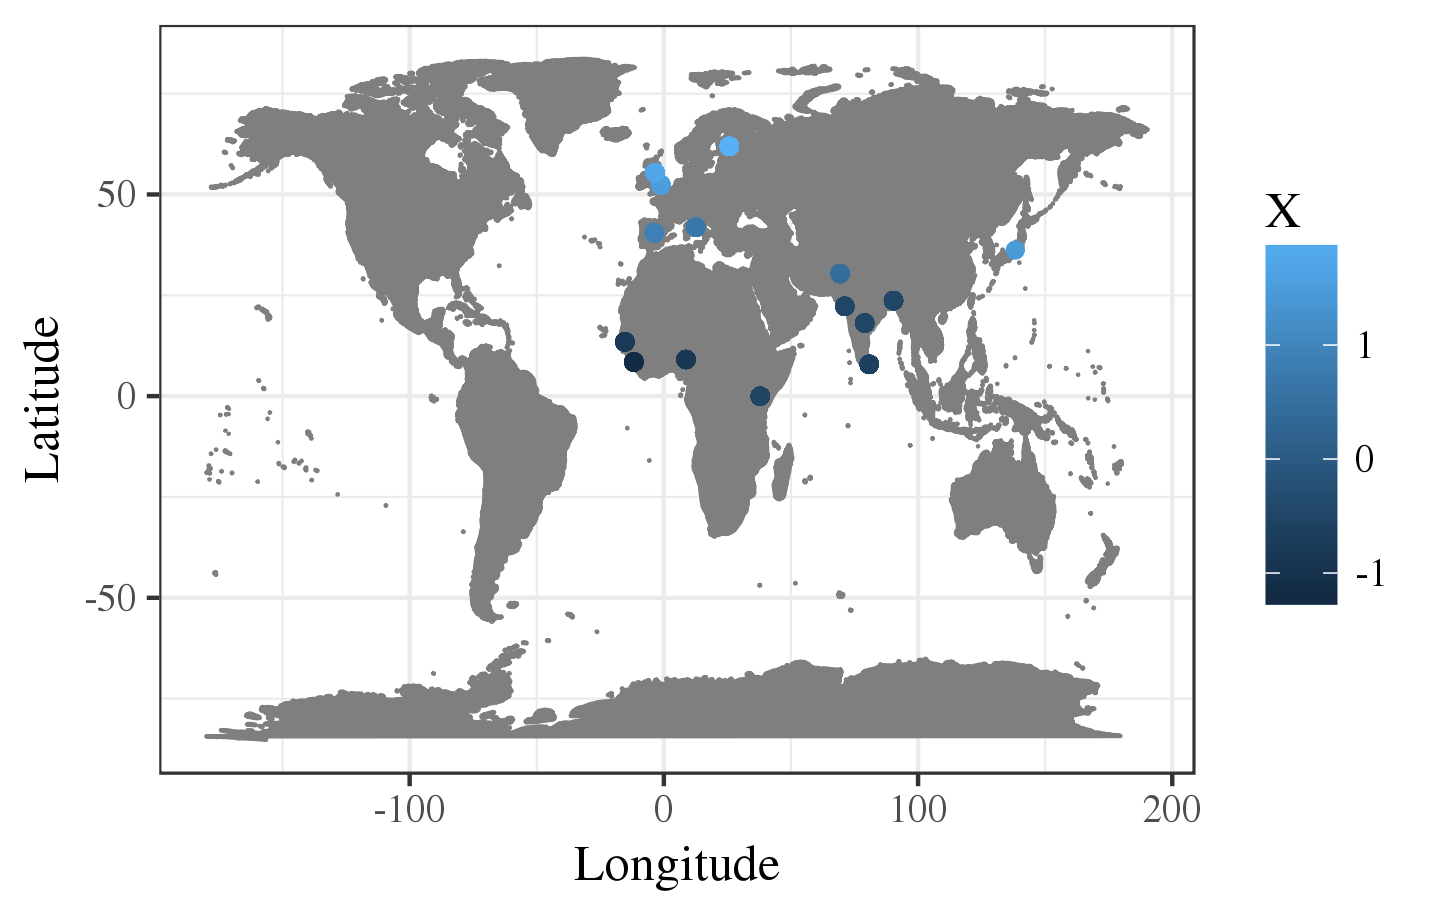
\includegraphics{./OUTPUT/Rplots/eas_climatic_gradient.pdf}
\caption{Gradient climatique $\X$ utilisé pour l'association génotypes-environnement.}
\label{fig:eas_gradient}
\end{figure}

\section{Résultats}
\label{sec:org33f3e6c}
Dans cette partie, nous présentons les expériences numériques que nous avons
réalisées, pour évaluer la performance de nos algorithmes de correction des
facteurs de confusion dans les études d'association. Les deux nouveaux
algorithmes ont été implémentés dans le langage de programmation R et sont
appelés respectivement ridgeLFMM pour l'estimation \(L_{2}\) et lassoLFMM pour
l'estimation \(L_{1}\). Nos méthodes sont comparées aux méthodes présentées dans
la partie \ref{orgb7a2d5c}. Les méthodes de régression linéaire avec et sans
les scores de l'ACP ont été implémentées dans le langage R. Elles sont
respectivement appelées lm et PCAlm. Pour les méthodes cate, sva-irw et
sva-two-step, nous avons respectivement utilisé les implémentations R mises à
disposition par leurs auteurs respectifs.
\subsection{Comparaison des méthodes sur des données simulées}
\label{sec:org64b1f78}
Sur les 125 jeux de données simulés, nous avons utilisé les méthodes lm, PCAlm,
sva-irw, sva-two-step, cate, les deux méthodes présentées dans ce chapitre
(lassoLFMM et ridgeLFMM) et la méthode oracle. Pour comparer les méthodes, nous
avons calculé les facteurs d'inflation et les aires sous la courbe
précision-rappel (AUC). Les méthodes cate, lassoLFMM et ridgeLFMM ont des
performances similaires à la méthode oracle sur toutes les simulations (Figure
\ref{fig:method_comp}), sauf lorsque paramètre de corrélation \(\rho\) vaut 1. En
effet, sur les simulations avec une forte corrélation entre les variables
latentes et la variable explicative, cate et ridgeLFMM renvoient des \pvalues
avec un taux d'inflation moyen de \(3.3\) alors que celui de lassoLFMM vaut \(1.3\)
et celui de l'oracle \(1.0\) (Figure \ref{fig:method_comp} D). Nous constatons par
ailleurs que les méthodes cate et ridgeLFMM donnent des résultats très
similaires sur toutes les simulations. Les performances de la méthode lm sont
sensibles au paramètre de corrélation \(\rho\). Lorsque le paramètre de
corrélation est faible, l'AUC de lm et le facteur d'inflation de lm sont proches
de ceux de la méthode oracle (\(\rho = 0.1\), Figure \ref{fig:method_comp} B et D).
Mais le facteur d'inflation de lm croît jusqu'à plus de 30 et l'AUC décroît
jusqu'à la moitié de celui de la méthode oracle lorsqu'il y a une forte
corrélation entre les variables latentes et la variable explicative (\(\rho = 1\),
Figure \ref{fig:method_comp} B et D). Les \pvalues de la méthode PCAlm sont
toujours correctement calibrées puisque le facteur d'inflation est toujours
autour de 1 (Figure \ref{fig:method_comp} C et D). Cependant l'écart de l'AUC de
PCAlm avec l'AUC obtenu par la méthode oracle croît avec la proportion de vraies
associations et le paramètre de corrélation \(\rho\) (Figure \ref{fig:method_comp} A
et B). Les méthodes sva-two-step et sva-irw renvoient des \pvalues correctement
calibrées sauf quand le paramètre de corrélation \(\rho\) vaut 0.8 et 1.0 (Figure
\ref{fig:method_comp} C et D). L'AUC de sva-irw est toujours en dessous de l'AUC
de la méthode oracle pour toutes les proportions de vraies associations dans les
simulations (Figure \ref{fig:method_comp} A). La différence entre l'AUC de sva-irw
et l'AUC de la méthode oracle croît avec le paramètre de corrélation \(\rho\)
(Figure \ref{fig:method_comp} B). Nous observons également que l'AUC de
sva-two-step est très légèrement en dessous de l'AUC de la méthode oracle pour
toutes les proportions de vraies associations dans les simulations (Figure
\ref{fig:method_comp} A) et, comme pour sva-irw, la différence de l'AUC de
sva-two-step avec l'AUC de la méthode oracle croît avec le paramètre de
corrélation \(\rho\) mais plus faiblement que pour sva-irw (Figure
\ref{fig:method_comp} B).

\begin{sidewaysfigure}
\centering
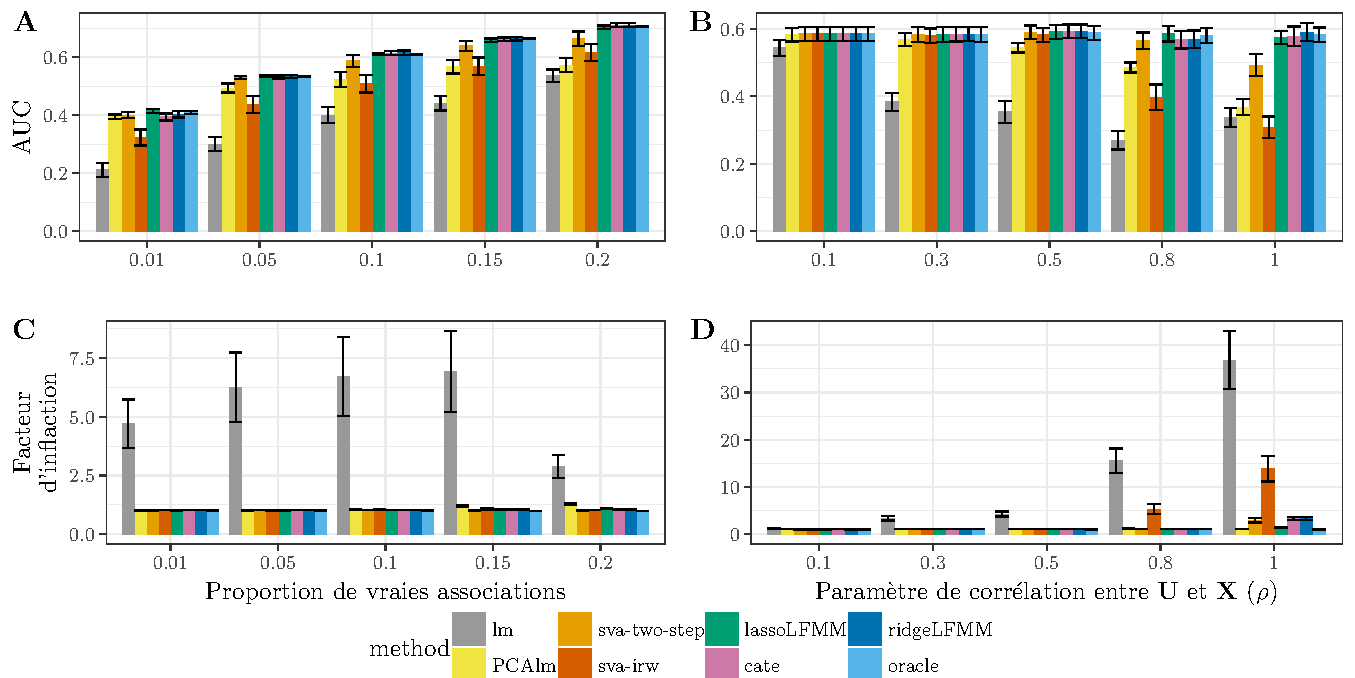
\includegraphics{./OUTPUT/Rplots/lfmm_method_comp.pdf}
\caption{{\bf Comparaison des méthodes sur des simulations rélisées à partir du jeu de
  données 1000Genomes.} A-B) Aire sous la courbe précision-rappel en fonction de
  la proportion de colonnes de $\Y$ associées à $\X$ et de la corrélation de la
  variable explicative $\X$ avec les variables latentes. C-D) Facteur
  d'inflation calculé sur les variables nulles en fonction de la proportion de
  colonnes de $\Y$ associées à $\X$ et la corrélation de la variable explicative
  $\X$ avec les variables latentes.}
\label{fig:method_comp}
\end{sidewaysfigure}

\subsection{Étude d'association entre des niveaux de méthylation de l'ADN et la polyarthrite rhumatoïde (EWAS)}
\label{sec:org7af9219}
\label{org30cf0b0} 

Nous avons appliqué les méthodes cate, lm, PCAlm, sva-irw, sva-two-step,
lassoLFMM et ridgeLFMM afin de trouver les sites de méthylation de l'ADN
associés à la polyarthrite. Nous avons choisi \(\K = 10\) pour le nombre de
variables latentes (voir Figure \ref{fig:ewas_params} A et B). Pour \(\K = 10\), les
valeurs du paramètre de régularisation \(L_{2}\) (\(\lambRidge\)) entre \(10^{-10}\)
et \(1.0\) donnent les mêmes valeurs moyennes d'erreur de prédiction (Figure
\ref{fig:ewas_params} C). Nous avons choisi de prendre \(\lambRidge = 10^{-5}\) pour
ridgeLFMM. 

\begin{figure}
\centering
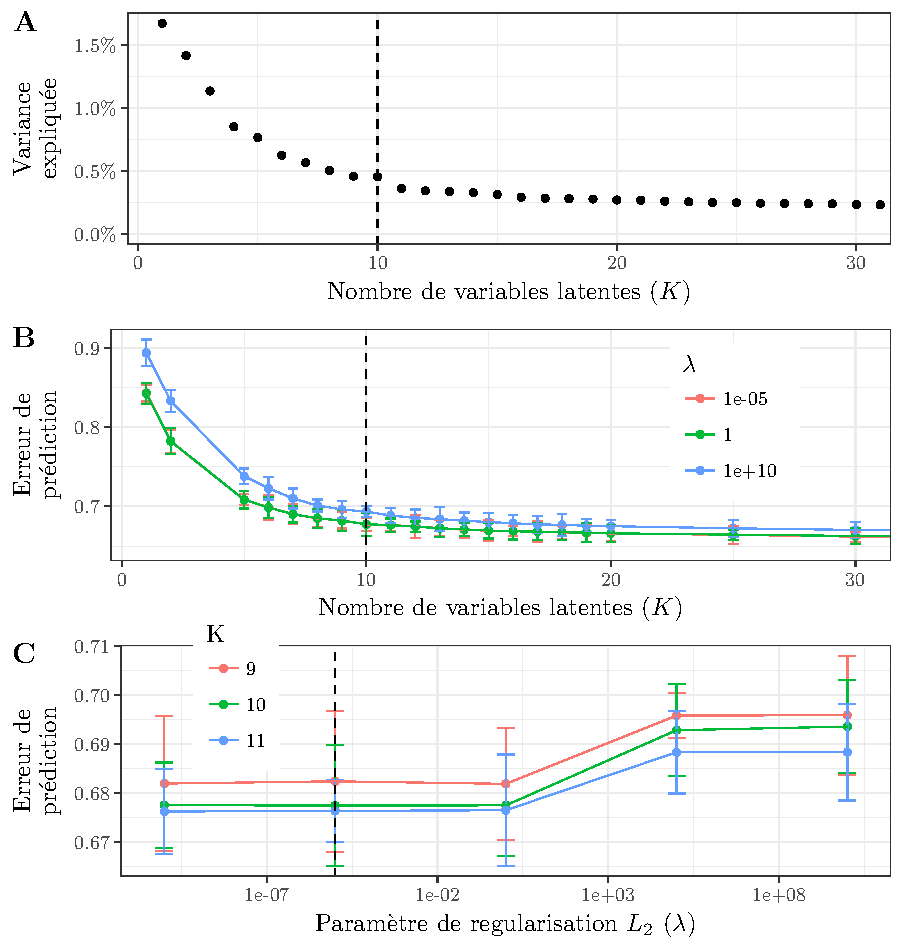
\includegraphics{./OUTPUT/Rplots/ewas_hyperparams.pdf}
\caption{{\bf Choix des paramètres pour l'étude d'association entre des sites
    méthylation de l'ADN et la polyarthrite rhumatoïde (EWAS).} A) Proportion de
  variance expliquée de la projection de $\Y$ sur l'espace orthogonal à $\X$
  (c'est à dire $\matr{D}_{0} \Q^{T} \Y$) par chacune des composantes
  principales. B)C) Erreur de prédiction calculée grâce à la validation croisée
  des estimateurs $L_{2}$ des paramètres de LFMM pour différente valeurs du
  paramètre de régularisation $\lambda$ et du nombre variable latentes $\K$. Le
  point représente l'erreur de prédiction moyen et les barres l'erreur standard.
  La ligne pointillée verticale marque sur A et B le nombre de variables
  latentes choisies, c'est à dire 10, et sur C le paramètre de régularisation
  choisi, c'est à dire $\lambda = 10^{-5}$. }
\label{fig:ewas_params}
\end{figure}

Nous constatons une augmentation du nombre de petites \pvalues pour toutes les
méthodes; cette augmentation est encore plus forte pour les méthodes lm et
sva-irw (Figure \ref{fig:ewas_qqplot_top} A). La figure \ref{fig:ewas_qqplot_top} B
montre la proportion des candidats identifiés par \citet{Zou_2014,Rahmani_2016}
qui sont retrouvés dans les listes rangées (les listes sont rangées selon les
\(p\text{-valeurs}\)) retournées par chaque méthode. Nous rappelons que les
candidats identifiés par \citet{Zou_2014,Rahmani_2016} sont au nombre de 5. Ils
ont été identifiés en prenant en compte les facteurs de confusion tels que
l'âge, le sexe et une estimation de la composition cellulaire. Les méthodes
considérées dans notre analyse retrouvent les candidats de la littérature dans
leurs 40 premiers rangs, sauf lm et sva-irw (Figure \ref{fig:ewas_qqplot_top} B).
Pour la méthode lm, il faut prendre le rang 11881 pour trouver le premier
candidat de \citet{Zou_2014,Rahmani_2016}, et le rang 138038 pour tous les avoir.
Pour la méthode sva-irw, les candidats de \citet{Zou_2014,Rahmani_2016} sont tous
identifiés entre les rangs \(5111\) et \(87659\).

\begin{figure}[!h]
\centering
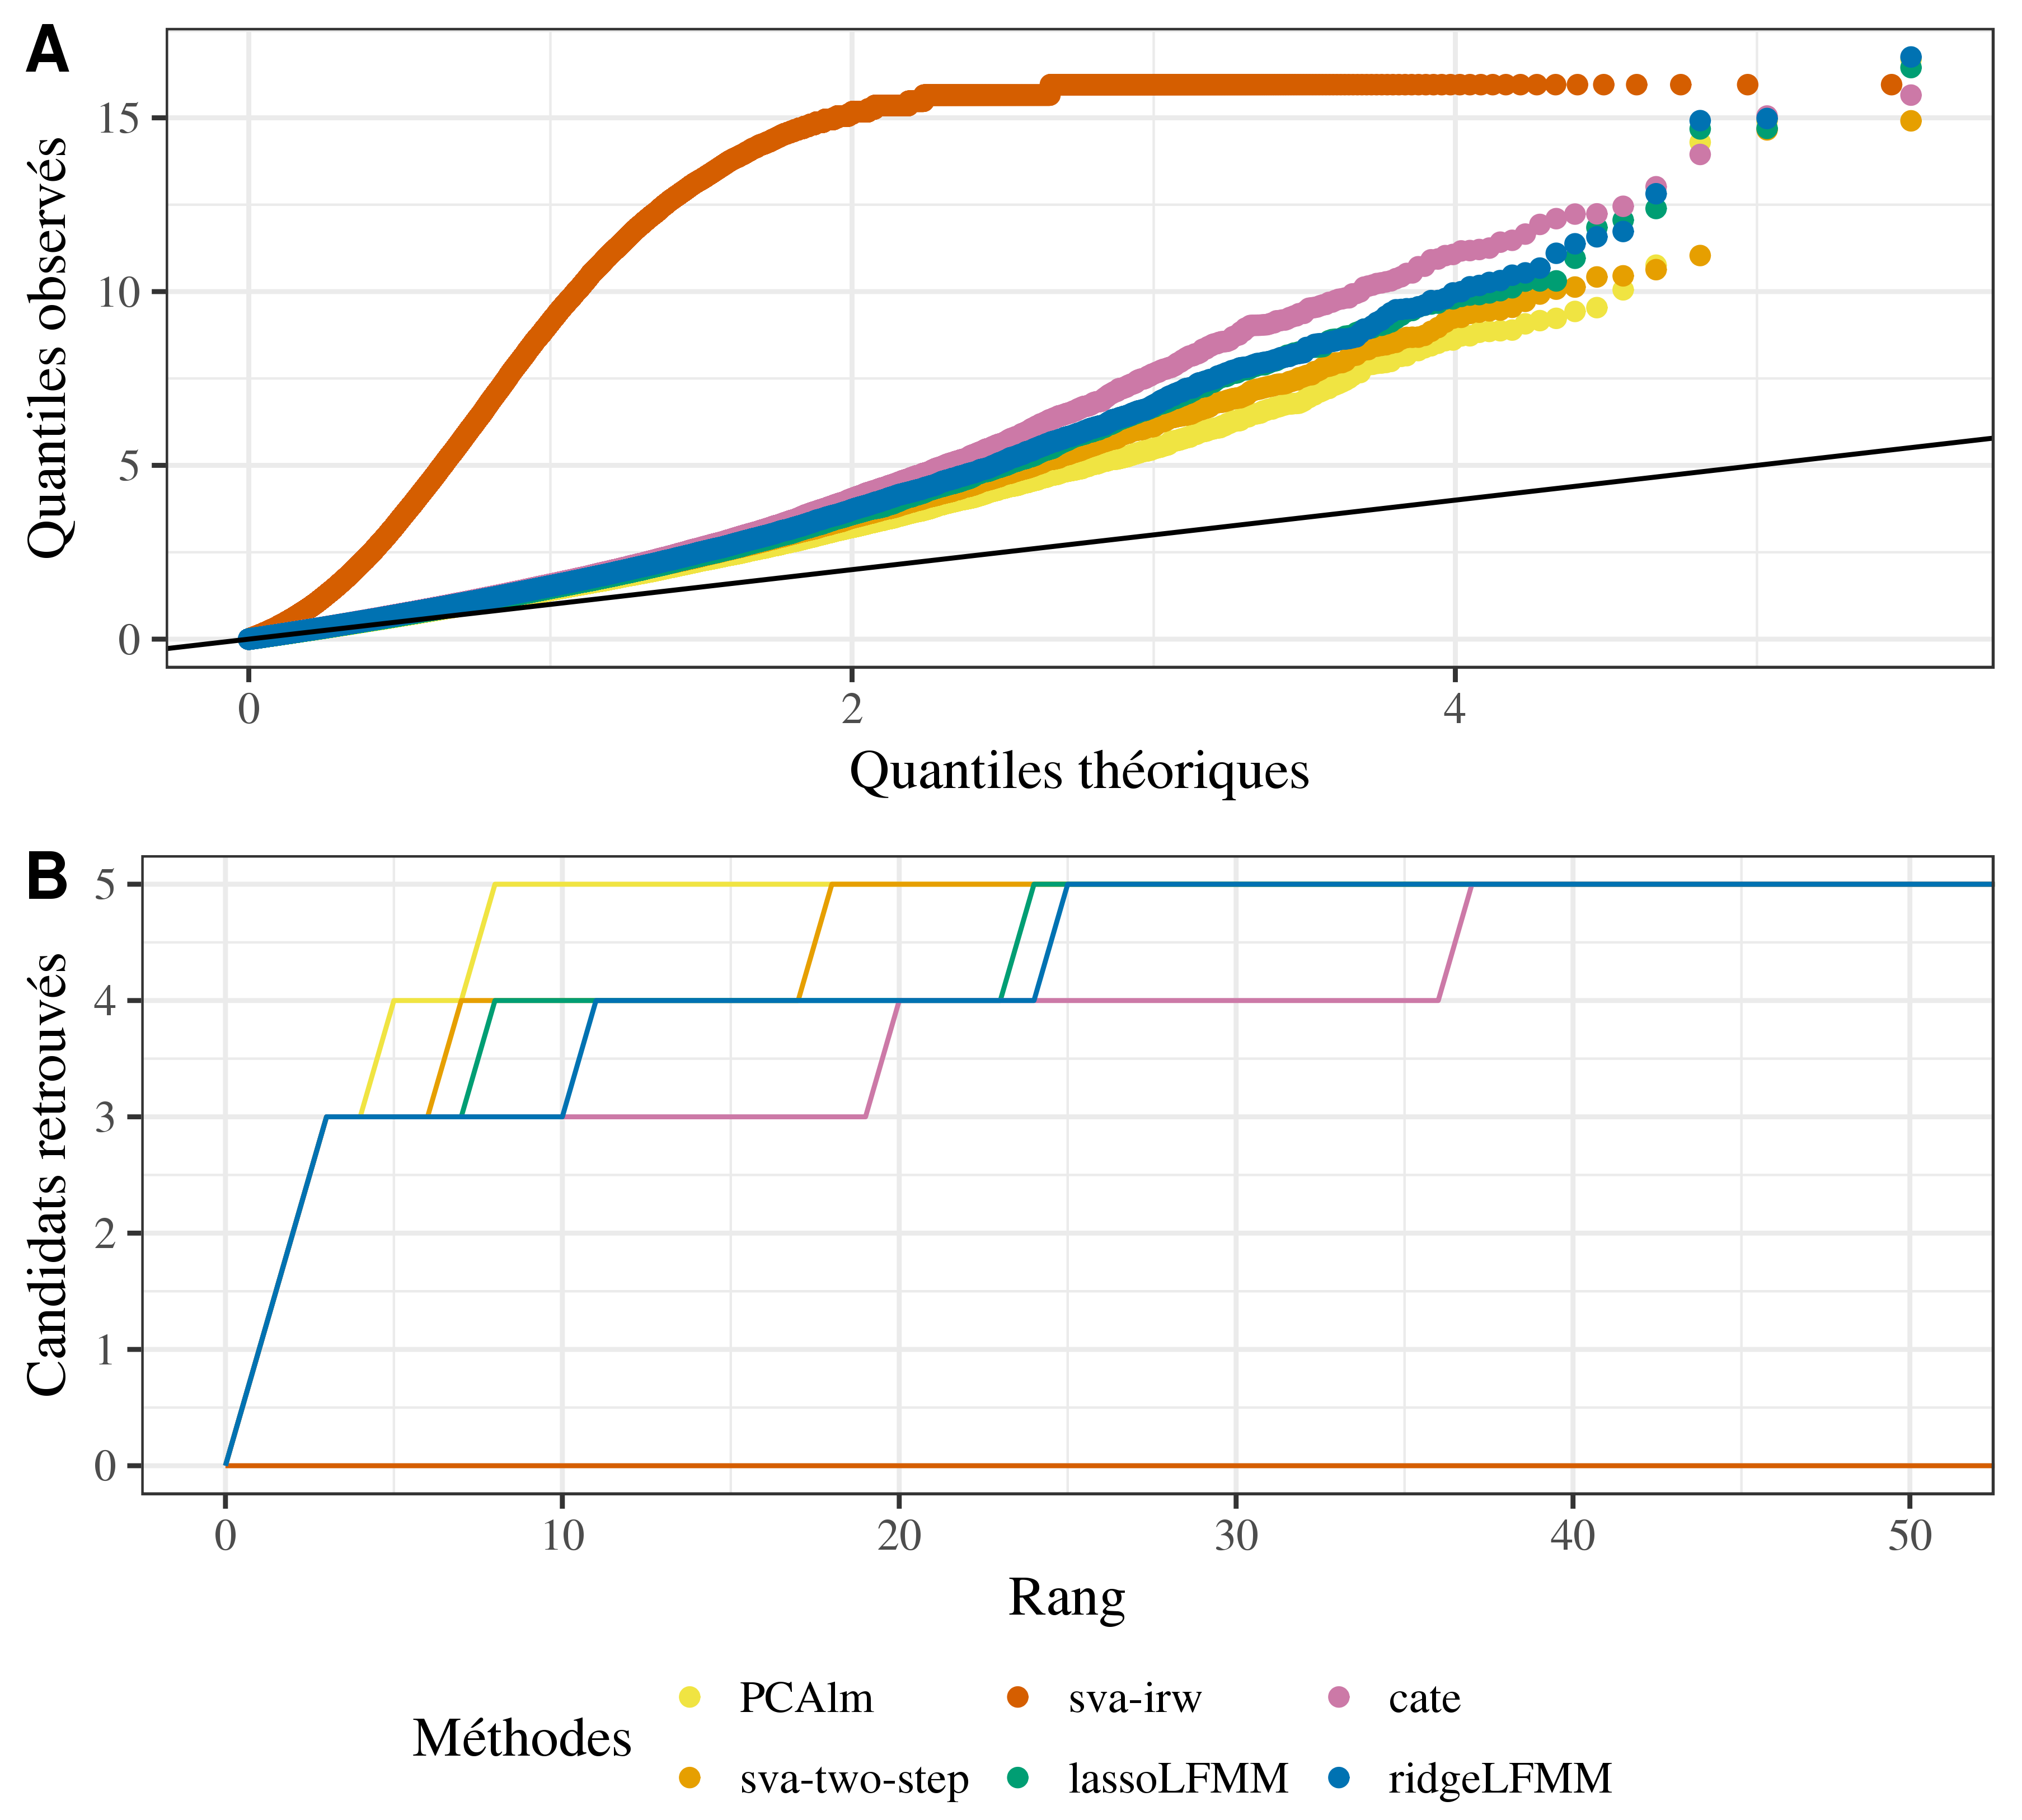
\includegraphics{./OUTPUT/Rplots/ewas_qqplot_top.png}
\caption{{\bf Q-Q plot et rang pour l'étude d'association entre des sites de
    méthylation et la polyarthrite rhumatoïde (EWAS).} A) Diagramme
  quantile-quantile de l'inverse du logarithme en base 10 des \pvalues renvoyées
  par chaque méthode. Les quantiles théoriques sont ceux de la loi
  exponentielle. B) Nombre de sites proposés par \citet{Rahmani_2016,Zou_2014}
  retrouvés dans la liste rangée (la liste est rangée selon les $p\text{-valeurs}$) avant
  un rang donné.}
\label{fig:ewas_qqplot_top}
\end{figure}

Enfin, nous calculons les sites de méthylation candidats pour l'association à la
polyarthrite lorsque l'on contrôle le taux de fausse découverte à \(1\%\). Nous
avons écarté lm et sva-irw car ils renvoyaient des listes trop différentes des
autres méthodes. Parmi les 19 candidats trouvés par toutes les méthodes lorsque
nous contrôlons le FDR à \(1 \%\), nous retrouvons les 5 candidats identifiés par
\citet{Zou_2014,Rahmani_2016}. Avec un FDR controlé à \(1 \%\), les méthodes PCAlm
et sva-two-step retournent des listes de 20 candidats avec 19 candidats en
commun. Les méthodes cate, lassoLFMM et ridgeLFMM proposent des listes de
candidats plus de deux fois plus longues que les méthodes PCAlm et sva-two-step.
De plus, les méthodes cate, lassoLFMM et ridgeLFMM proposent en commun 51 sites
de méthylation (Figure \ref{fig:ewas_venn}). Enfin, nous remarquons que d'autres
sites de méthylation situés dans des gènes sont détectés avant les 5 candidats
de la littérature. En particulier, nous trouvons des gènes situés dans le
complexe de gènes HLA qui joue un rôle central dans le système immunitaire
(Table \ref{table:ewas}).

\begin{figure}[!h]
\centering
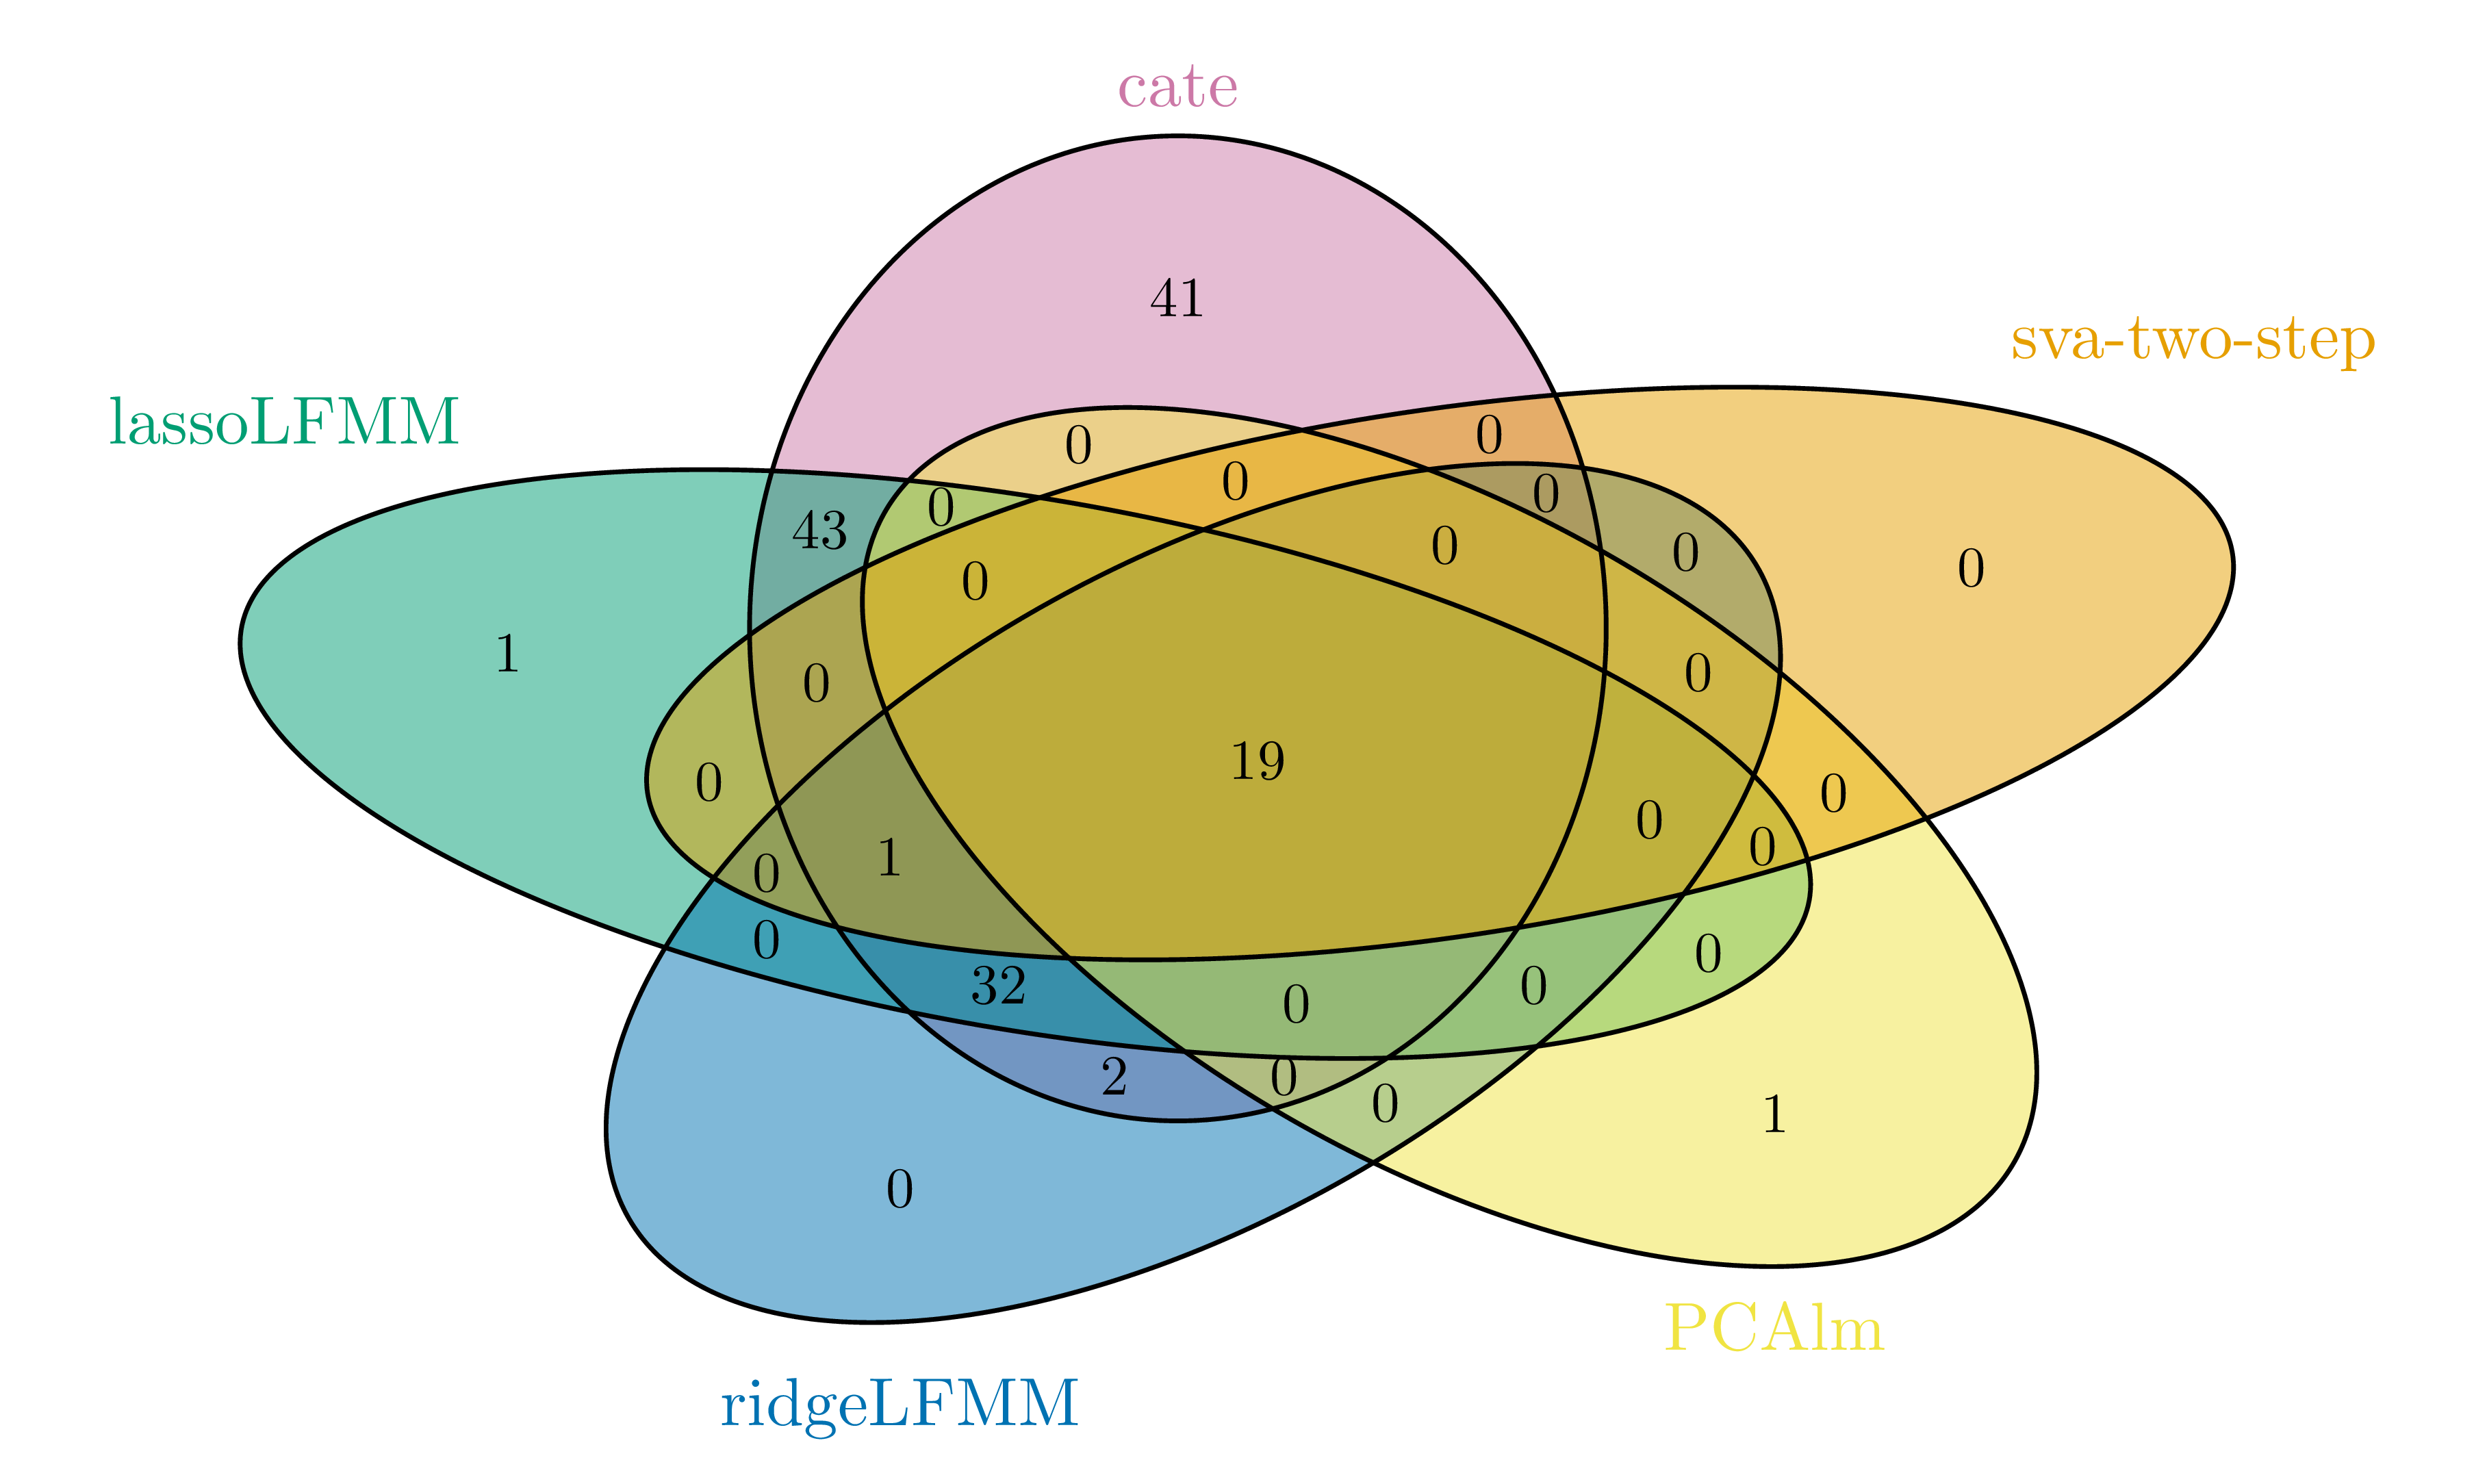
\includegraphics[width=\textwidth]{./OUTPUT/Rplots/ewas_venn.png}
\caption{{\bf Diagramme de Venn de l'étude d'association entre des sites de
    méthylation et la polyarthrite rhumatoïde (EWAS).} Diagramme de Venn des
  listes controlées à un taux de fausses de découvertes de 1 \%.}
\label{fig:ewas_venn}
\end{figure}

\rowcolors{2}{gray!25}{white}
% latex table generated in R 3.4.0 by xtable 1.8-2 package
% Sun Oct  8 20:25:36 2017
\begin{sidewaystable}[ht]
\centering
\begin{tabular}{llllcccc}
  \hline
ID & Chr & Position & Gene & PCAlm & lassoLFMM & cate & ridgeLFMM \\ 
  \hline
\textbf{cg16411857} & \textbf{16} & \textbf{57023191} & \textbf{NLRC5} & \textbf{9.2e-13} & \textbf{2.4e-12} & \textbf{6.6e-12} & \textbf{5.3e-12} \\ 
  \textbf{cg07839457} & \textbf{16} & \textbf{57023022} & \textbf{NLRC5} & \textbf{1.9e-11} & \textbf{4.5e-11} & \textbf{1.1e-10} & \textbf{9.7e-11} \\ 
  \textbf{cg05428452} & \textbf{6} & \textbf{32712979} & \textbf{HLA-DQA2} & \textbf{5.4e-11} & \textbf{4.6e-11} & \textbf{8.5e-11} & \textbf{8.8e-11} \\ 
  cg02508743 & 8 & 56903623 & LYN & 2.9e-08 & 2.7e-08 & 2.7e-08 & 2.8e-08 \\ 
  \textbf{cg20821042} & \textbf{6} & \textbf{32709158} & \textbf{HLA-DQA2} & \textbf{6.5e-08} & \textbf{6.1e-08} & \textbf{9.6e-08} & \textbf{1.0e-07} \\ 
  cg13081526 & 6 & 32449961 &  & 1.5e-07 & 1.2e-07 & 2.0e-07 & 2.2e-07 \\ 
  cg18052547 & 6 & 32552547 & HLA-DRB1 & 1.8e-07 & 1.8e-07 & 3.0e-07 & 3.1e-07 \\ 
  \textbf{cg25372449} & \textbf{6} & \textbf{32490350} & \textbf{HLA-DRB5} & \textbf{2.5e-07} & \textbf{2.6e-07} & \textbf{4.5e-07} & \textbf{4.6e-07} \\ 
  cg02030958 & 13 & 110386267 &  & 4.0e-07 & 7.8e-08 & 6.0e-08 & 1.1e-07 \\ 
  cg16171858 & 3 & 58472734 &  & 4.6e-07 & 1.6e-07 & 2.7e-08 & 3.8e-08 \\ 
  cg03280622 & 8 & 145023013 & PLEC1 & 4.7e-07 & 5.0e-09 & 5.8e-09 & 3.8e-08 \\ 
  cg24150157 & 19 & 51891210 & LIM2 & 6.2e-07 & 3.1e-07 & 1.6e-07 & 2.1e-07 \\ 
  cg26244575 & 12 & 76354015 &  & 6.9e-07 & 2.7e-09 & 5.0e-10 & 4.2e-09 \\ 
  cg05370853 & 6 & 32606634 & HLA-DQA1 & 7.1e-07 & 3.0e-07 & 3.3e-07 & 4.4e-07 \\ 
  cg14989316 & 10 & 80757927 & LOC283050 & 7.3e-07 & 6.1e-08 & 7.8e-08 & 2.1e-07 \\ 
  cg17360552 & 6 & 32725332 & HLA-DQB2 & 8.1e-07 & 6.1e-07 & 1.1e-06 & 1.2e-06 \\ 
  cg01373248 & 3 & 18480297 & SATB1 & 8.1e-07 & 1.4e-07 & 1.1e-07 & 2.5e-07 \\ 
  cg26164488 & 2 & 64440295 &  & 9.3e-07 & 3.5e-09 & 1.6e-09 & 1.4e-08 \\ 
  cg05874806 & 2 & 102350276 & MAP4K4 & 1.1e-06 & 1.1e-06 & 4.7e-07 & 5.6e-07 \\ 
   \hline
\end{tabular}
\caption{{\bf Sites de méthylation associés avec la maladie polyarthrite rhumatoïde (EWAS).} \pvalues des candidats détectés par les méthodes PCAlm, lassoLFMM, ridgeLFMM et cate pour un taux de fausse décourverte controlé à 1$\%$ pour l'EWAS. Les Sites de méthylation en gras sont les candidats de \citep{Zou_2014, Rahmani_2016}} 
\label{table:ewas}
\end{sidewaystable}

\subsection{Étude d'association entre des données génétiques et la maladie c\oe{}liaque (GWAS)}
\label{sec:orgad47ebb}

Nous avons utilisé les méthodes cate, lm, PCAlm, lassoLFMM et ridgeLFMM afin de
trouver les SNPs associés avec la maladie \celiac. Nous avons utilisé les
méthodes avec 9 variables latentes (Figure \ref{fig:gwas_params} A et B). La
validation croisée du paramètre \(\lambRidge\) tend à sélectionner une forte
valeur pour celui-ci (Figure \ref{fig:gwas_params} C). La validation croisée
présentée sur la Figure \ref{fig:gwas_params} C sélectionne une valeur plus grande
que \(10^3\). Nous avons choisi \(10^3\) car, comme nous l'avons discuté dans la
partie \ref{org4dbaae9}, \(\lambRidge\) trop grand conduit la méthode ridgeLFMM à
renvoyer les mêmes résultats que PCAlm.

\begin{figure}[!h]
\centering
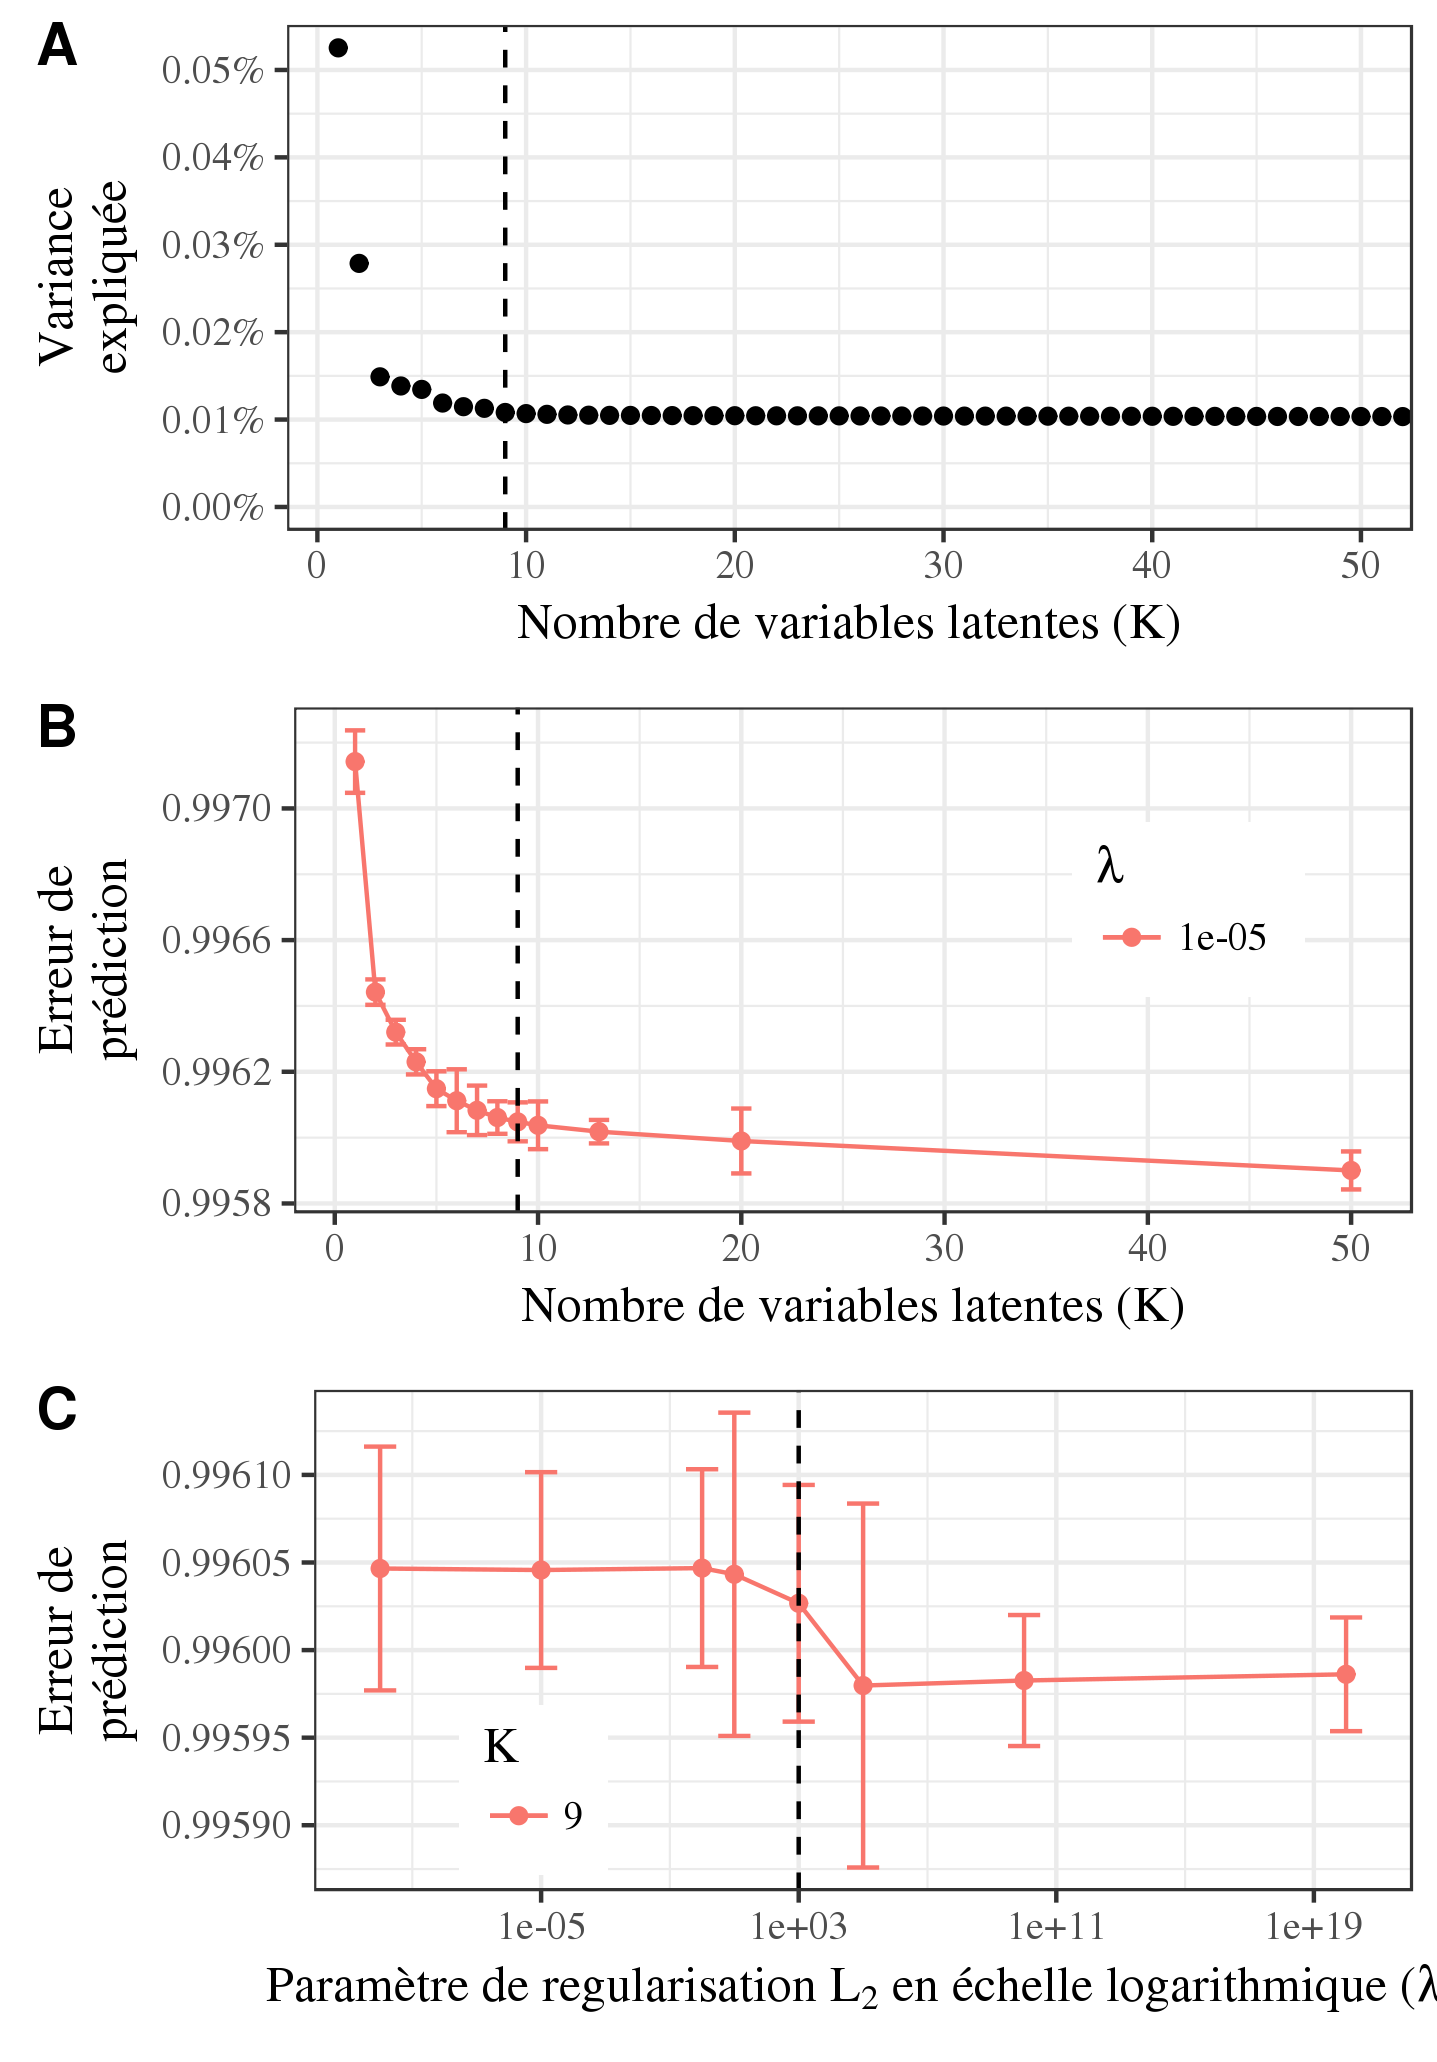
\includegraphics{./OUTPUT/Rplots/gwas_hyperparams.pdf}
\caption{{\bf Choix des paramètres pour l'étude d'association entre génotype et
    la maladie c\oe{}liaque (GWAS).}  A) Proportion de variance expliquée de la
  projection de $\Y$ sur l'espace orthogonal à $\X$ (c'est à dire $\matr{D}_{0}
  \Q^{T} \Y$) par chacune des composantes principales. B)C) Erreur de prédiction
  calculée grâce à la validation croisée des estimateurs $L_{2}$ des paramètres
  de LFMM pour différente valeurs du paramètre de régularisation $\lambda$ et du
  nombre variable latentes $\K$. Le point représente l'erreur de prédiction
  moyen et les barres l'erreur standard. La ligne pointillée verticale marque
  sur A et B le nombre de variables latentes choisies, c'est à dire 9, et sur C
  le paramètre de régularisation choisi, c'est à dire $\lambda = 10^{-3}$. }
\label{fig:gwas_params}
\end{figure}

Les méthodes fournissent des \pvalues bien calibrées avec une forte inflation du
nombre de petites \pvalues (Figure \ref{fig:gwas_qqplot_top} A). La méthode la
plus libérale est lm, alors que ridgeLFMM et PCAlm sont les méthodes les plus
conservatives. Le chromosome 6 contient le complexe de gènes HLA. Ce complexe de
gènes joue un rôle important dans le système immunitaire et dans la maladie
c\oe{}liaque \citep{dubois2010multiple}. Nous avons séparé les SNPs candidats du
GWAS catalog retrouvés sur le chromosome 6 des autre chromosomes. Les candidats
du GWAS catalog sur le chromosome 6 arrive plus tôt dans les listes rangées (la
liste est rangée selon les \(p\text{-valeurs}\)) des méthodes PCAlm et ridgeLFMM (Figure
\ref{fig:gwas_qqplot_top} B). Sur les autres chromosomes, ce sont les méthodes
lassoLFMM et cate qui retrouvent le plus vite les candidats du GWAS catalog
(Figure \ref{fig:gwas_qqplot_top} B).

\begin{figure}[!h]
\centering
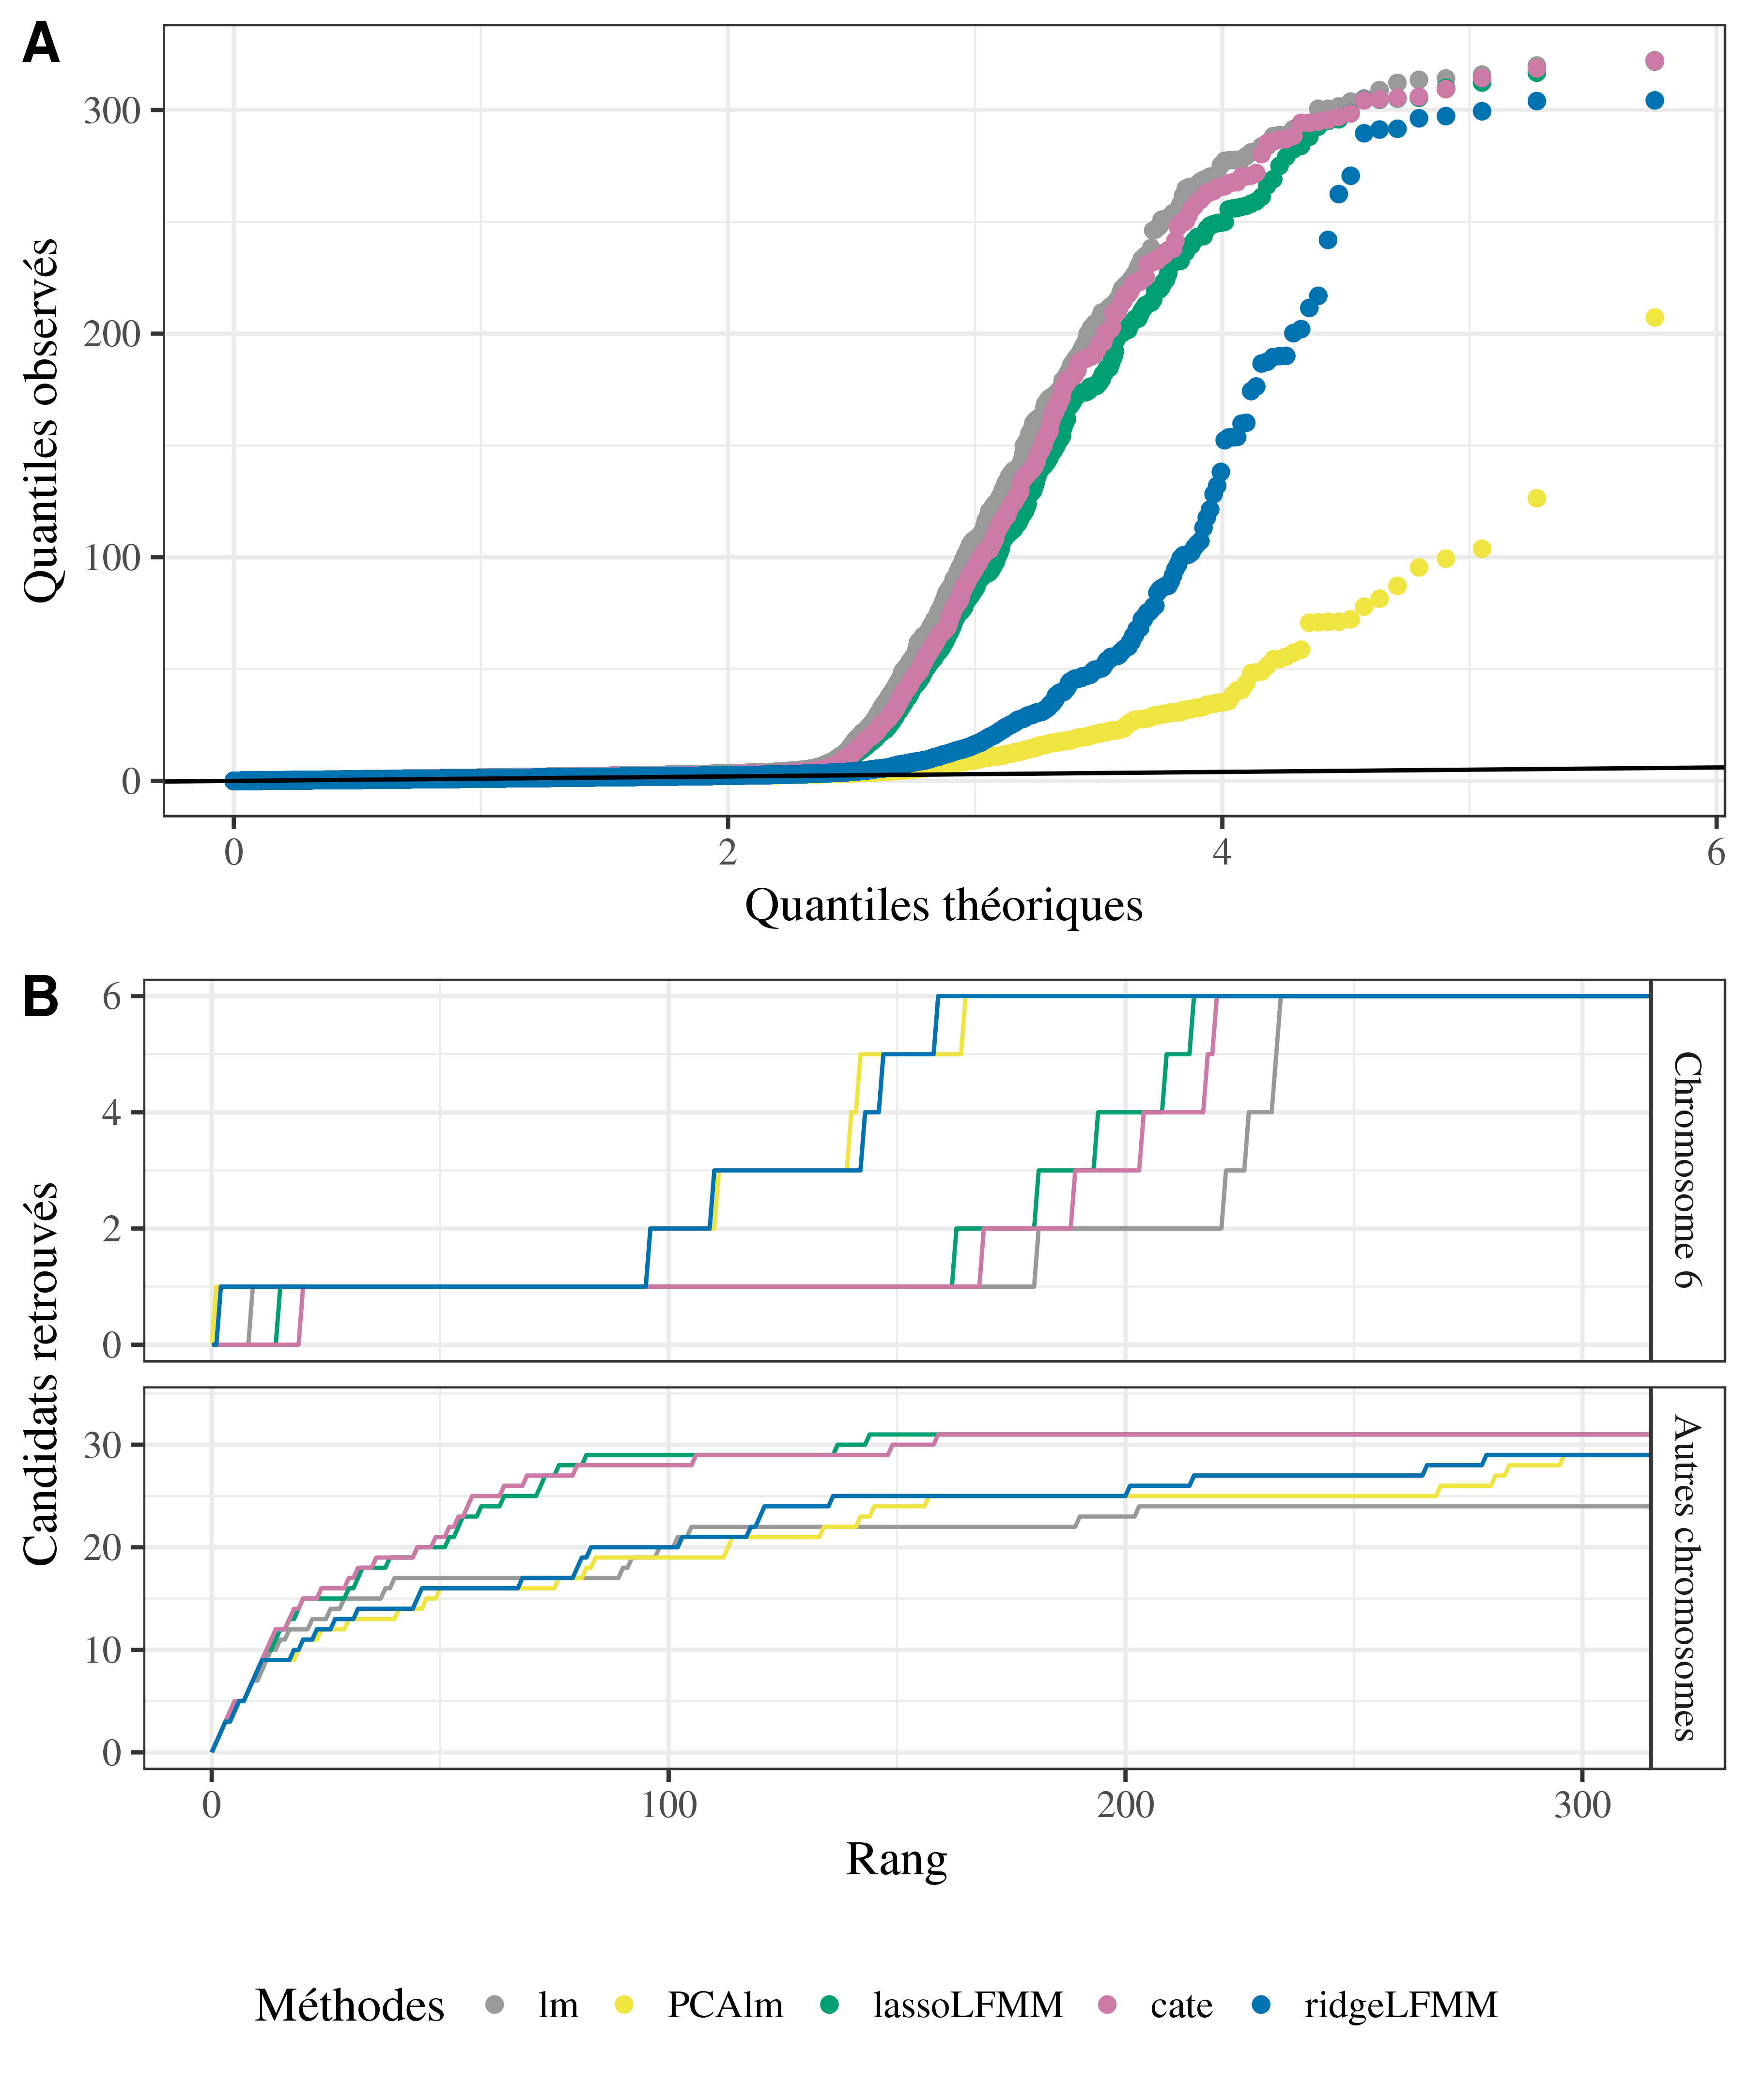
\includegraphics{./OUTPUT/Rplots/gwas_qqplot_top.png}
\caption{{\bf Q-Q plot et rang pour l'étude d'association entre des génomes et
    la maldie c\oe{}liaque (GWAS).} A) Diagramme quantile-quantile de l'inverse
  du logarithme en base 10 des \pvalues renvoyées par chaque méthode. Les
  quantiles théoriques sont ceux de la loi exponentielle. B) Nombre de gènes du
  GWAS catalog retrouvés dans la liste rangée (la liste est rangée selon les $p\text{-valeurs}$) avant
  un rang donné.}
\label{fig:gwas_qqplot_top}
\end{figure}

Enfin, nous calculons les SNPs candidats pour l'association à la maladie
\celiac lorsque l'on contrôle le taux de fausse découverte à \(1\%\). Ce sont
ridgeLFMM et PCAlm qui donnent les plus petites listes contrôlées avec 754
candidats pour ridgeLFMM et 777 candidats pour PCAlm (Figure \ref{fig:gwas_venn}).
Les méthodes cate et lm donnent les plus grandes listes avec le même nombre de
1319 candidats. Nous constatons que l'intersection des listes à FDR contrôlé de
toutes les méthodes contient \(28\%\) des candidats du GWAS catalog. Afin
d'identifier des groupes de SNPs associés à la maladie \celiac, nous avons
regroupé les SNPs voisins corrélés grâce à l'algorithme de \emph{clumping} du
logiciel \texttt{plink}. Dans les 20 premières zones détectées par lassoLFMM, en dehors
du chromosome 6, 6 zones ne sont pas référencés dans le GWAS catalog (Table
\ref{table:gwas_table}).

\begin{figure}[!h]
\centering
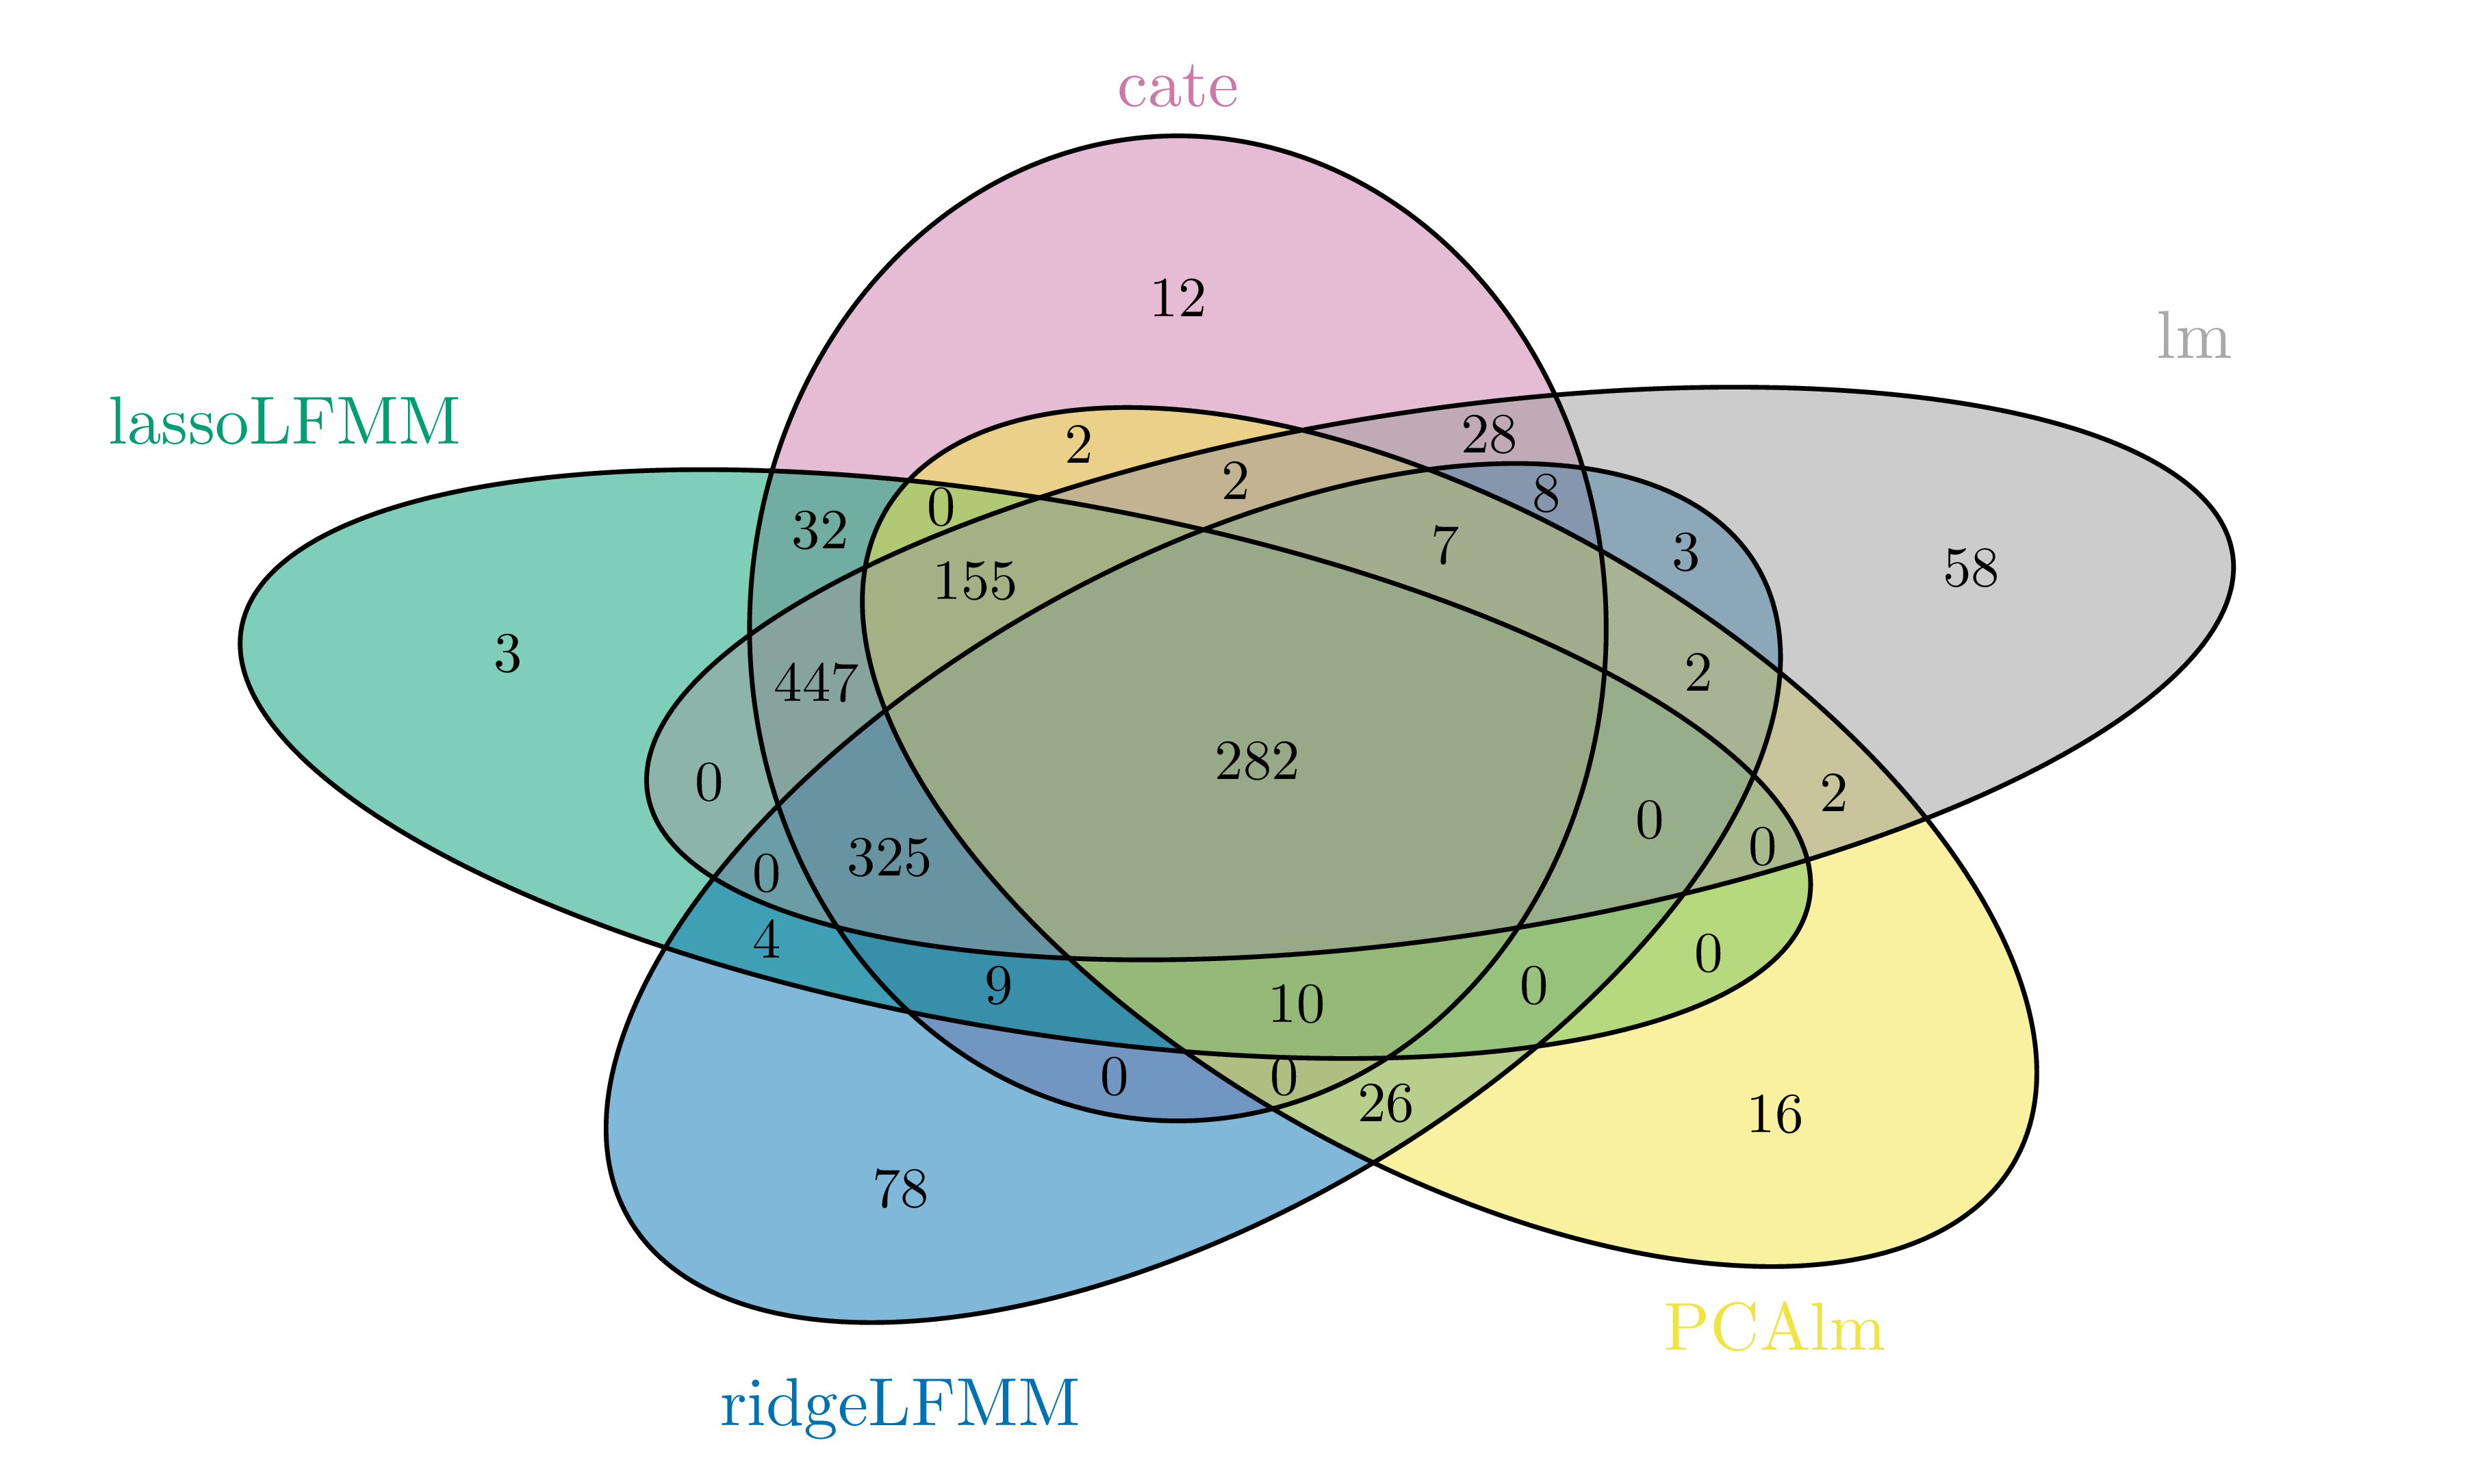
\includegraphics[width=\textwidth]{./OUTPUT/Rplots/gwas_venn.png}
\caption{{\bf Diagramme de Venn de l'étude d'association entre des génotypes et
    la maladie c\oe{}liaque (GWAS).} Diagramme de Venn des listes controlées à
  un taux de fausses de découvertes de $1 \%$ pour chaque méthode.}
\label{fig:gwas_venn}
\end{figure}

\rowcolors{2}{gray!25}{white}
% latex table generated in R 3.4.0 by xtable 1.8-2 package
% Tue Oct 10 18:00:18 2017
\begin{sidewaystable}[ht]
\centering
\begingroup\fontsize{8pt}{8pt}
\begin{tabular}{llllccp{6cm}}
  \hline
Chr & Snp & LD block (Mb) & Odds ratio [$95\%$ IC] & \pvalue & \qvalue & Gènes dans la zone \\ 
  \hline
\textbf{3} & \textbf{rs1464510} & \textbf{189.56-189.61} & \textbf{1.30 [1.24-1.36]} & \textbf{3.8e-23} & \textbf{1.5e-20} & \textbf{LPP} \\ 
  \textbf{3} & \textbf{rs17810546} & \textbf{160.99-161.32} & \textbf{1.35 [1.26-1.45]} & \textbf{1.8e-16} & \textbf{6.1e-14} & \textbf{IQCJ-SCHIP1, IL12A-AS1, IL12A} \\ 
  \textbf{4} & \textbf{rs13151961} & \textbf{123.19-123.56} & \textbf{0.73 [0.68-0.78]} & \textbf{1.7e-14} & \textbf{5.3e-12} & \textbf{KIAA1109, ADAD1} \\ 
  \textbf{12} & \textbf{rs653178} & \textbf{110.25-110.49} & \textbf{1.22 [1.16-1.28]} & \textbf{6.8e-13} & \textbf{2.1e-10} & \textbf{CUX2, LINC02356, SH2B3, ATXN2} \\ 
  \textbf{2} & \textbf{rs917997} & \textbf{102.26-102.61} & \textbf{1.27 [1.20-1.35]} & \textbf{1.5e-12} & \textbf{4.6e-10} & \textbf{IL1RL1, IL18R1, IL18RAP, MIR4772, SLC9A4, SLC9A2} \\ 
  4 & rs6840978 & 123.73-123.77 & 0.77 [0.72-0.82] & 1.2e-11 & 3.5e-09 & IL21-AS1 \\ 
  3 & rs9811792 & 161.12-161.18 & 1.18 [1.12-1.24] & 6.6e-11 & 1.9e-08 & IL12A-AS1 \\ 
  \textbf{3} & \textbf{rs13098911} & \textbf{45.98-46.21} & \textbf{1.32 [1.22-1.43]} & \textbf{2.1e-10} & \textbf{5.8e-08} & \textbf{FYCO1, FLT1P1, CCR3} \\ 
  \textbf{1} & \textbf{rs2816316} & \textbf{190.77-190.80} & \textbf{0.78 [0.72-0.83]} & \textbf{2.2e-10} & \textbf{6.2e-08} & \textbf{} \\ 
  \textbf{3} & \textbf{rs6441961} & \textbf{46.26-46.33} & \textbf{1.21 [1.15-1.27]} & \textbf{1.7e-08} & \textbf{4.6e-06} & \textbf{CCR3, UQCRC2P1} \\ 
  \textbf{2} & \textbf{rs4675374} & \textbf{204.29-204.52} & \textbf{1.23 [1.16-1.31]} & \textbf{2.1e-07} & \textbf{5.4e-05} & \textbf{CD28, ICOS} \\ 
  2 & rs1018326 & 181.54-181.78 & 1.15 [1.10-1.21] & 4.4e-07 & 1.1e-04 & UBE2E3, LINC01934 \\ 
  3 & rs7648827 & 46.56-46.56 & 1.22 [1.12-1.33] & 4.6e-07 & 1.2e-04 & LRRC2 \\ 
  \textbf{2} & \textbf{rs13003464} & \textbf{60.95-61.24} & \textbf{1.19 [1.13-1.25]} & \textbf{5.0e-07} & \textbf{1.3e-04} & \textbf{LINC01185, REL, PUS10, RNA5SP95, KIAA1841, C2orf74} \\ 
  \textbf{10} & \textbf{rs1250552} & \textbf{80.71-80.74} & \textbf{0.84 [0.80-0.88]} & \textbf{5.2e-07} & \textbf{1.3e-04} & \textbf{ZMIZ1} \\ 
  3 & rs7629708 & 189.56-189.62 & 1.17 [1.11-1.24] & 1.0e-06 & 2.5e-04 & LPP \\ 
  \textbf{22} & \textbf{rs2298428} & \textbf{20.13-20.31} & \textbf{1.17 [1.10-1.24]} & \textbf{1.3e-06} & \textbf{3.3e-04} & \textbf{HIC2, UBE2L3, YDJC, CCDC116} \\ 
  18 & rs1394466 & 48.93-49.30 & 1.14 [1.08-1.20] & 1.5e-06 & 3.6e-04 & DCC \\ 
  \textbf{18} & \textbf{rs1893217} & \textbf{12.80-12.84} & \textbf{1.16 [1.08-1.23]} & \textbf{1.6e-06} & \textbf{4.0e-04} & \textbf{PTPN2} \\ 
  \textbf{1} & \textbf{rs864537} & \textbf{165.66-165.70} & \textbf{0.87 [0.83-0.92]} & \textbf{1.7e-06} & \textbf{4.2e-04} & \textbf{POU2F1, CD247} \\ 
   \hline
\end{tabular}
\endgroup
\caption{{\bf 20 premiers groupes de SNPs associés avec la maladie \coeliac retrounés par l'algorithme lassoLFMM.} Les lignes en gras sont les SNPs référencés dans la base de données GWAS catalog.} 
\label{table:gwas_table}
\end{sidewaystable}
\subsection{Étude d'association entre des données génétiques et un gradient environnemental (GEAS)}
\label{sec:org431eb88}
\label{orgedaebe0}

Nous avons utilisé les méthodes cate, ridgeLFMM, lassoLFMM et PCAlm avec 9
variables latentes, afin de trouver les SNPs associés à un gradient climatique.
Nous avons utilisé les méthodes avec 9 variables latentes (Figure
\ref{fig:eas_params} A et B). Le screeplot et l'erreur de validation croisée
conduisent à choisir 5 variables latentes, mais nous avons choisi un nombre
légèrement plus élevé car les individus proviennent de 16 populations
différentes. En effet, les 6 premières variables latentes permettent d'expliquer
la structure de population (Figure \ref{fig:eas_variable} A et B). Les variables
latentes 8 et 9 ne permettent pas de visualiser la structure de population, mais
il pourrait s'agir de facteurs de confusion à prendre en compte dans l'étude
d'association (Figure \ref{fig:eas_variable} C). Enfin, les 10-ième et 11-ième
variables latentes séparent un seul individu du reste du groupe (Figure
\ref{fig:eas_variable} D), nous avons donc choisi \(K = 9\). Pour \(\K = 9\), les
valeurs du paramètre de régularisation \(L_{2}\) comprises entre \(10^{-10}\)
et \(1.0\) donnent les mêmes valeurs moyennes d'erreur de prédiction (Figure
\ref{fig:eas_params} C). Nous avons choisi de prendre \(\lambRidge = 10^{-5}\) pour
ridgeLFMM.

\begin{figure}[!h]
\centering
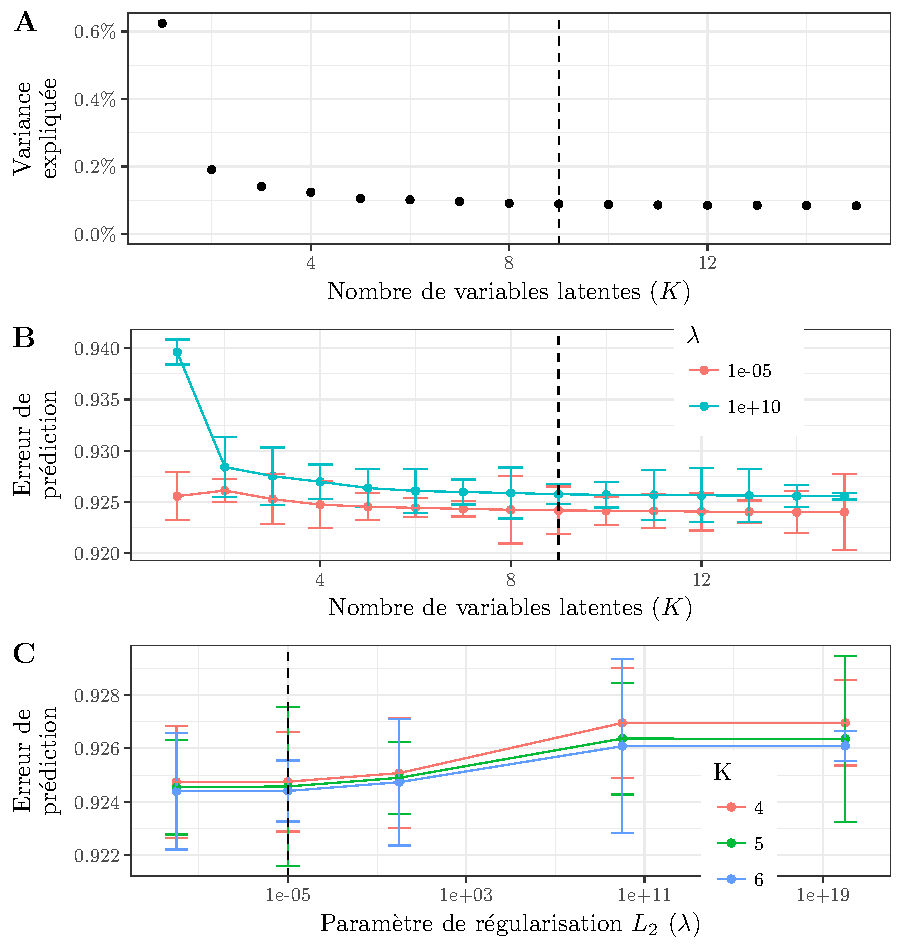
\includegraphics{./OUTPUT/Rplots/eas_hyperparams.pdf}
\caption{{\bf Choix des paramètres pour l'étude d'association entre génotype et
    un gradient environnemental (GEAS).} A) Proportion de variance expliquée de
  la projection de $\Y$ sur l'espace orthogonal à $\X$ (c'est à dire
  $\matr{D}_{0} \Q^{T} \Y$) par chacune des composantes principales. B)C) Erreur
  de prédiction calculée grâce à la validation croisée des estimateurs $L_{2}$
  des paramètres de LFMM pour différente valeurs du paramètre de régularisation
  $\lambda$ et du nombre variable latentes $\K$. Le point représente l'erreur de
  prédiction moyen et les barres l'erreur standard. La ligne pointillée
  verticale marque sur A et B le nombre de variables latentes choisies, c'est à
  dire 9, et sur C le paramètre de régularisation choisi, c'est à dire $\lambda
  = 10^{-3}$. }
\label{fig:eas_params}
\end{figure}

\begin{figure}[!h]
\centering
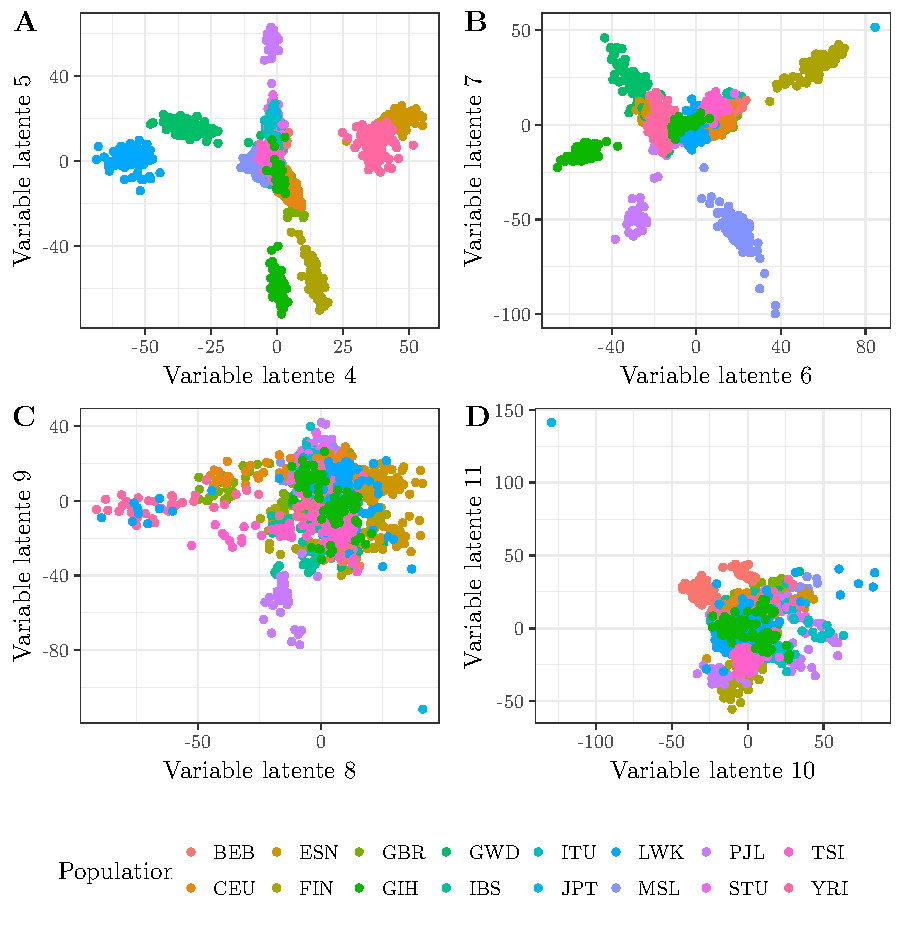
\includegraphics{./OUTPUT/Rplots/eas_pc.pdf}
\caption{{\bf Variables latentes retournées par ridgeLFMM pour l'étude
    d'association entre génotype et un gradient environnemental (GEAS).} Les noms de populations sont les codes utilisés dans le projet 1000Genomes.}
\label{fig:eas_variable}
\end{figure}

La figure \ref{fig:geas_qqplot} montre la distribution observée des \pvalues
renvoyées par chaque méthode, contre la distribution théorique sous l'hypothèse
nulle. Nous constatons une forte inflation pour les petites \pvalues de la
méthode lm. En effet, le MAD des \zscores retournées par la méthode lm est de
\(8.7\). De plus nous remarquons que le diagramme quantile-quantile de lm forme
une droite. Cela signifie que même si nous recalibrons les \pvalues retournées
par la méthode lm, celle-ci ne permet pas d'identifier des \pvalues atypiques et
donc des candidats pour l'association. Par contre, nous observons un excès de
\pvalues atypiques pour les autre méthodes. Pour les méthodes PCAlm, ridgeLFMM,
lassoLFMM et cate, nous avons calculé la liste des SNPs candidats pour
l'association au gradient climatique, lorsque nous contrôlons le FDR à \(1
\%\). La méthode lm a été écartée pour les raisons que nous venons d'évoquer. La
Figure \ref{fig:gwas_venn} montre l'intersection des listes de candidats contrôlés
à un FDR de \(1\%\) entre les méthodes. L'union des candidats retournés par ces
quatre méthodes donne 836 SNPs. Nous avons étudié la sur-représentation de
chacun des degrés d'annotation de vep dans la sous-liste des 836 SNPs par
rapport à la liste complète de SNPs. Nous constatons qu'il y a en proportion 22
fois plus d'annotation \HIGH$\backslash$, 8 fois plus de \MODERATE$\backslash$ et \(1.7\) fois plus de
\LOW$\backslash$ dans les 836 SNPs que parmi les 5397214 SNPs. Nous avons de plus testé si
chaque rapport de proportion est significativement supérieur à 1 à l'aide d'un
test exact de Fisher; les trois tests renvoient une \pvalue inférieure à
\(0.005\). Ainsi, parmi les SNPs que nous proposons pour l'association aux
conditions climatiques, il y a une sur-représentation significative de
polymorphismes ayant des impacts forts sur l'expression des gènes. Enfin, dans
l'union des candidats, nous observons 21 SNPs référencés dans le GWAS catalog
pour être associés à différents phénotypes liés à l'environnement (Table
\ref{table:geas}). Nous remarquons qu'aucun SNP référencé dans le GWAS catalog
n'est détecté par les méthodes lm et PCAlm.

\begin{figure}[!h]
\centering
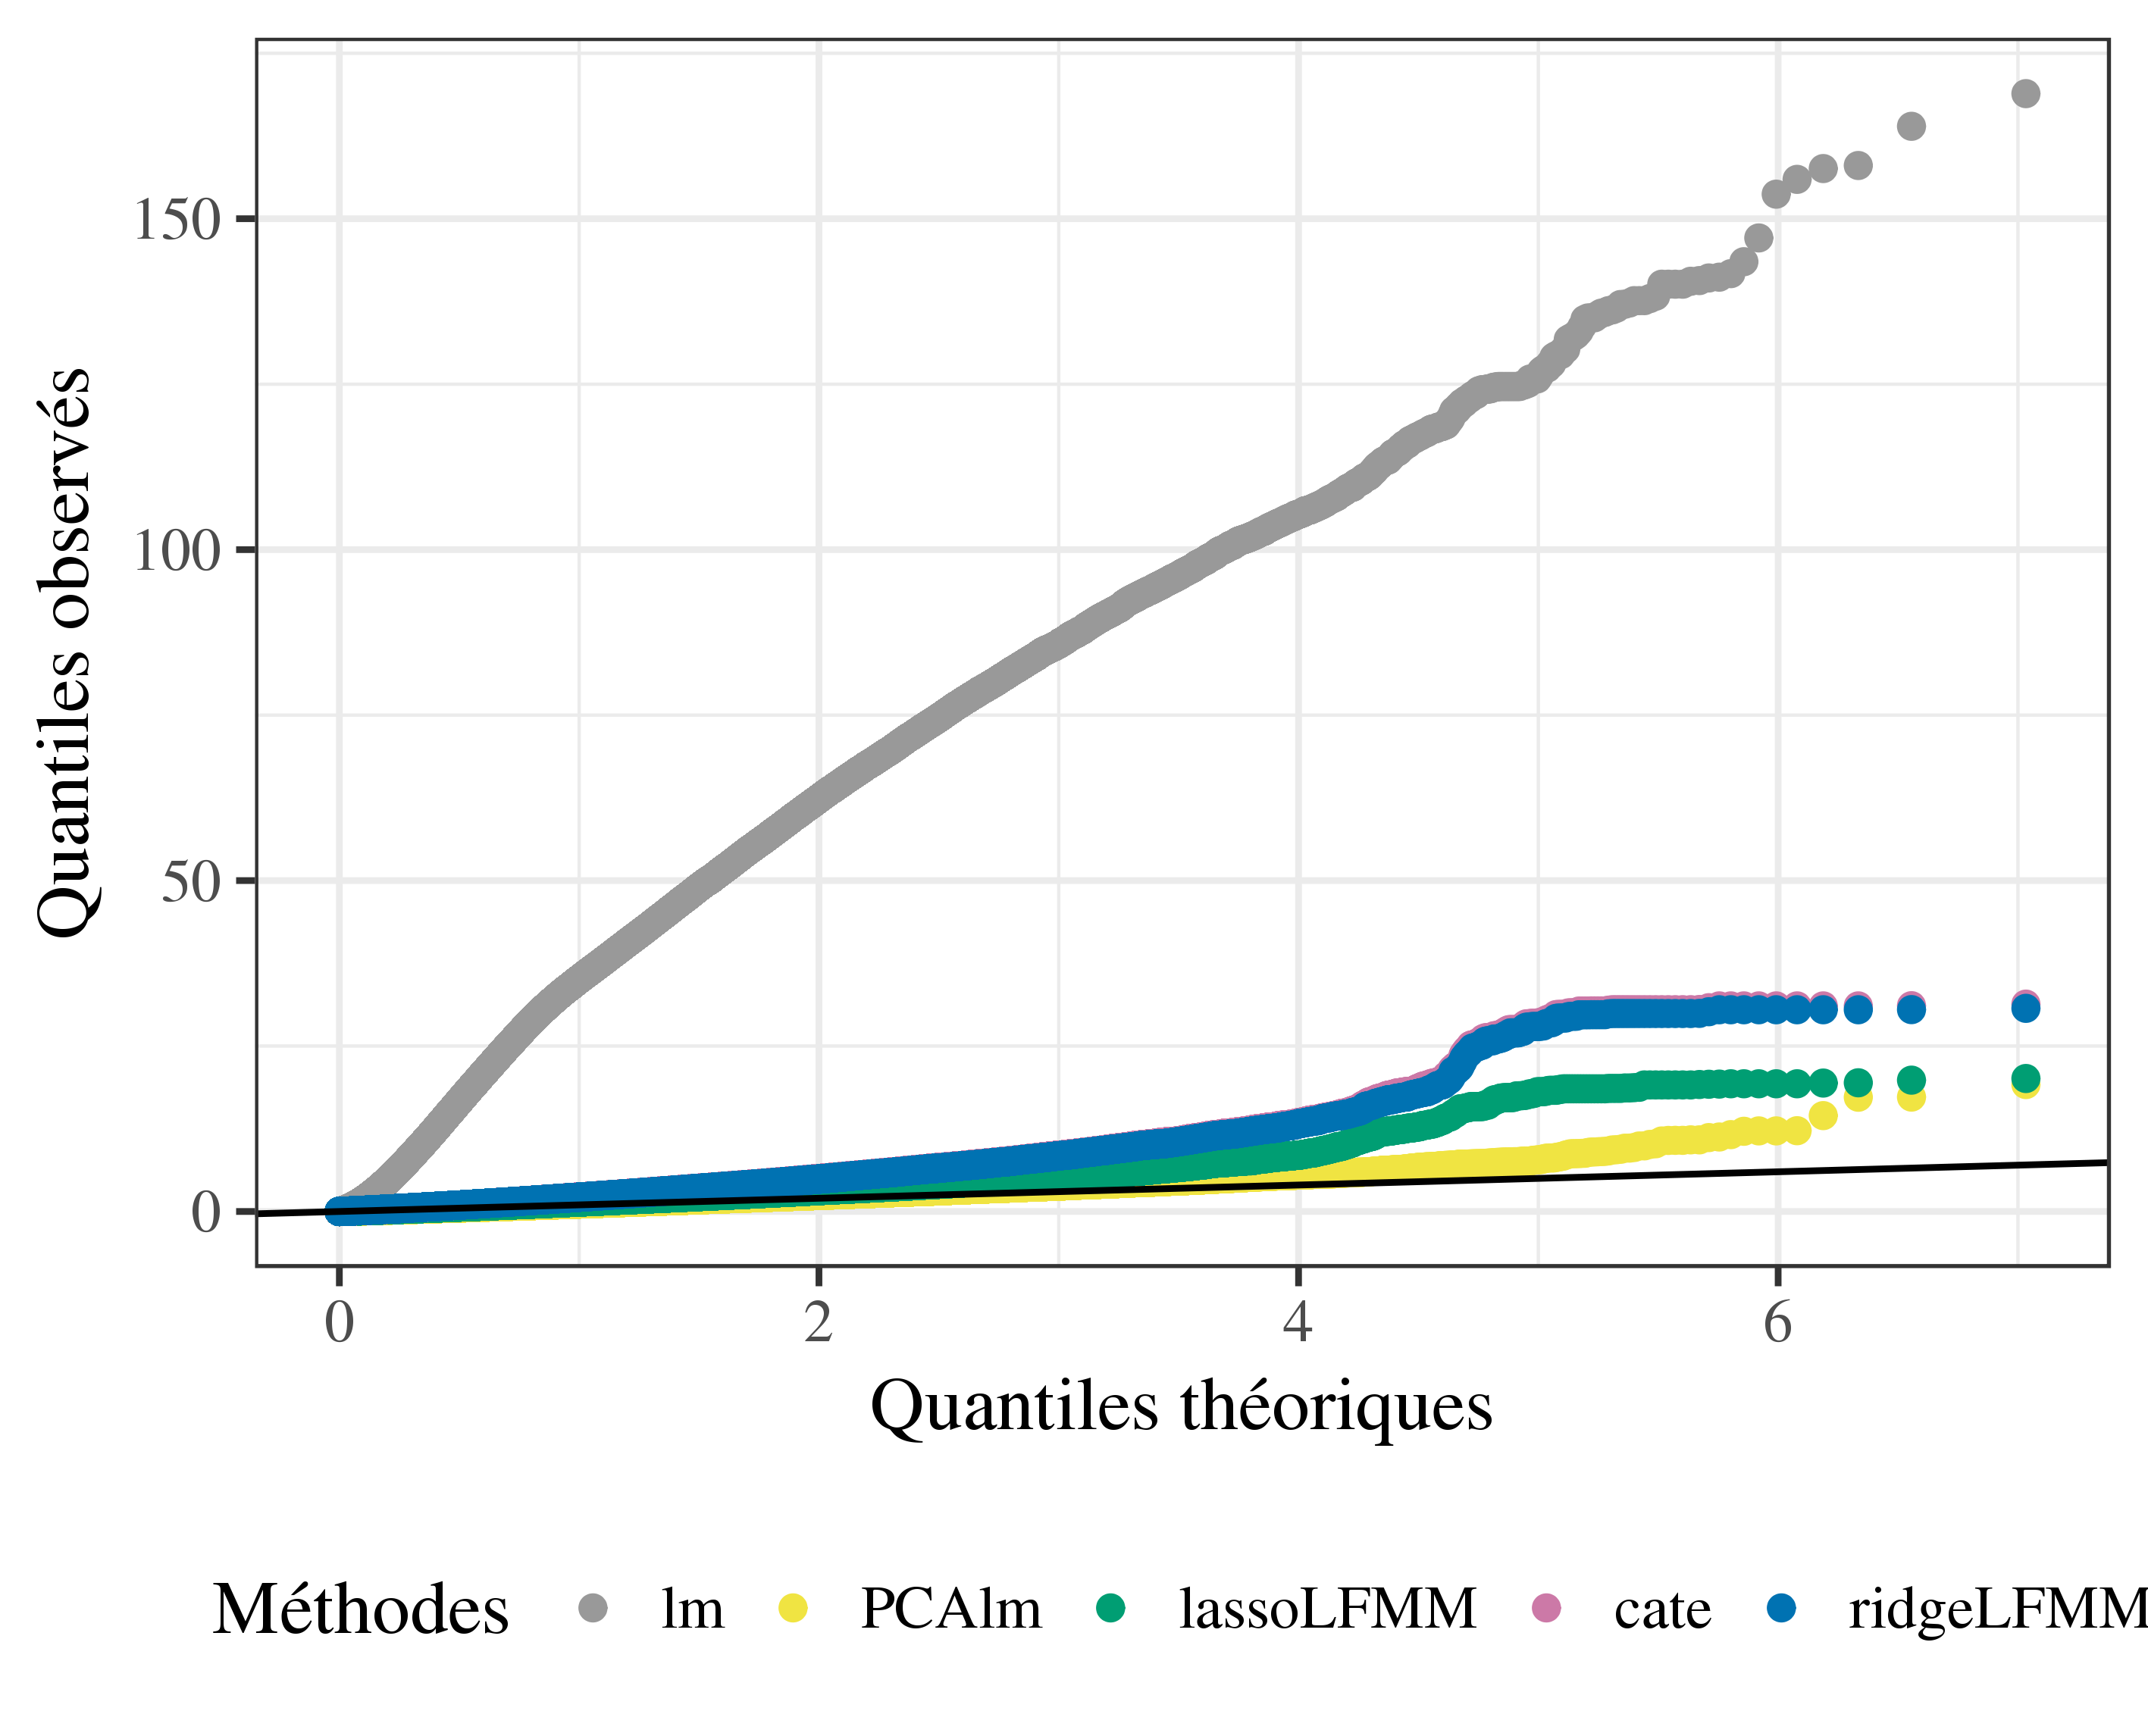
\includegraphics[width = \textwidth]{./OUTPUT/Rplots/geas_qqplot.png}
\caption{{\bf Q-Q plot de l'étude d'association entre génotype et un gradient
    environnemental (GEAS).} Diagramme quantile-quantile de l'inverse du
  logarithme en base 10 des \pvalues renvoyées par chaques méthodes. Les quantiles
  théoriques suivent la loi exponentielle.}
\label{fig:geas_qqplot}
\end{figure}

\begin{figure}[!h]
\centering
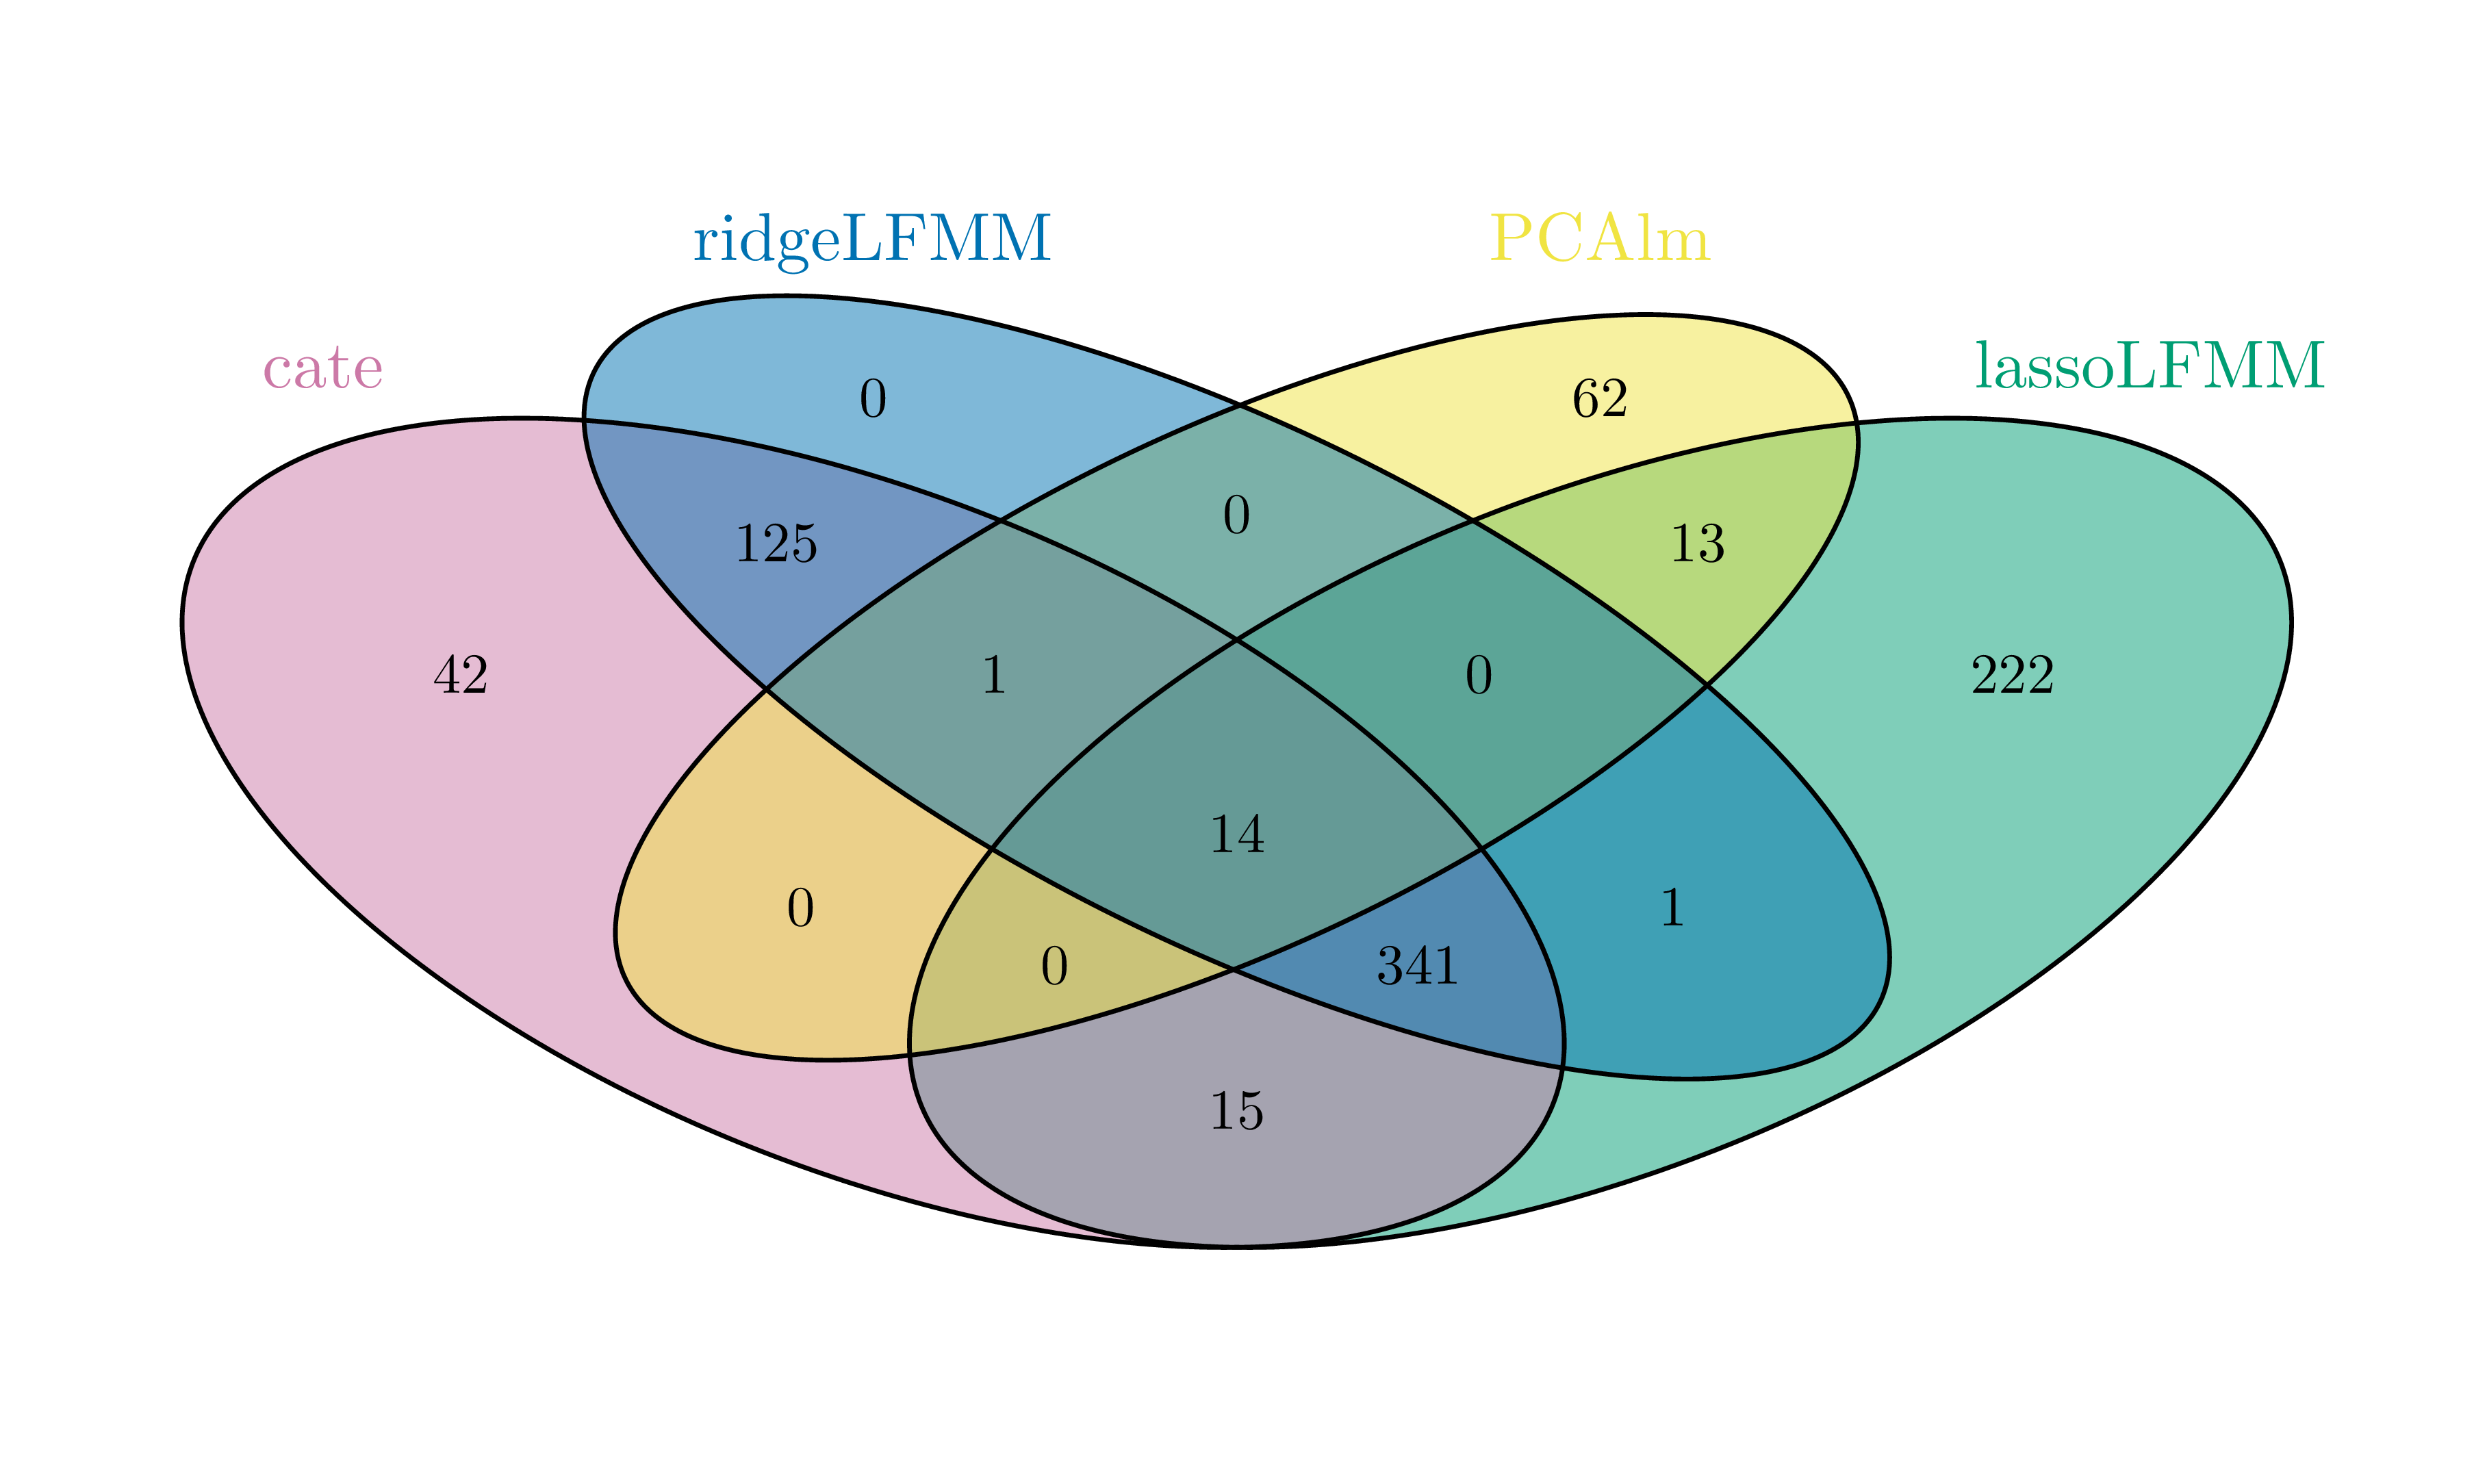
\includegraphics[width=\textwidth]{./OUTPUT/Rplots/geas_venn.png}
\caption{{\bf Diagramme de Venn de l'étude d'association entre des génotypes et
    un gradient environnemental (GEAS).} Diagramme de Venn des listes controlées à
  un taux de fausses de découvertes de $1 \%$ pour chaque méthode.}
\label{fig:geas_venn}
\end{figure}


\rowcolors{2}{gray!25}{white}
% latex table generated in R 3.4.0 by xtable 1.8-2 package
% Mon Oct  2 18:05:16 2017
\begin{sidewaystable}[ht]
\centering
\begin{tabular}{p{4cm}ll}
  \hline
SNPs & Détecté par les méthodes & Description du phénotype \\ 
  \hline
rs10908907 & ridgeLFMM, cate & Alcoholism (heaviness of drinking) \\ 
  rs10496731 & lassoLFMM & Body Height \\ 
  rs2472297 & ridgeLFMM, cate, lassoLFMM & Caffeine metabolism \\ 
  rs2256175 & ridgeLFMM, cate, lassoLFMM & Cholesterol total \\ 
  rs2472297 & ridgeLFMM, cate, lassoLFMM & Coffee consumption (cups per day) \\ 
  rs2278544, rs2322659 & lassoLFMM & Congenital lactase deficiency \\ 
  rs4954218 & ridgeLFMM, cate, lassoLFMM & Corneal structure \\ 
  rs882300 & ridgeLFMM, cate, lassoLFMM & Electrocardiographic traits \\ 
  rs882300 & ridgeLFMM, cate, lassoLFMM & Electrocardiography \\ 
  rs2256175 & ridgeLFMM, cate, lassoLFMM & Giant cell arteritis \\ 
  rs2256175, rs6085576, rs2104012, rs1983716, rs2853977 & ridgeLFMM, cate, lassoLFMM & Height \\ 
  rs6430549 & ridgeLFMM, cate, lassoLFMM & Hematocrit \\ 
  rs2278544, rs2322659 & lassoLFMM & Lactose intolerance \\ 
  rs882300 & ridgeLFMM, cate, lassoLFMM & Multiple sclerosis \\ 
  rs1123848 & ridgeLFMM, cate, lassoLFMM & Neuroblastoma \\ 
  rs17158483 & lassoLFMM & Obesity-related traits \\ 
   \hline
\end{tabular}
\caption{{\bf SNPs associés avec un gradient climatique qui ont été associés avec des phénotypes dans d'autres études.} SNPs présents dans l'union des SNPs détectés par les méthodes lassoLFMM, ridgeLFMM, cate et PCAlm pour un le FDR à $1\%$.} 
\label{table:geas}
\end{sidewaystable}

\section{Discussion}
\label{sec:org7064ae6}
Les études d'association sont largement utilisées en biologie pour trouver des
liens de corrélation entre des variables d'intérêt. Nous nous sommes intéressés
à la situation où des variables non observées expliquent une partie des
variations des variables expliquées et sont corrélées aux variables
explicatives. Nous avons proposé dans ce chapitre deux algorithmes, ridgeLFMM et
lassoLFMM, pour corriger les études d'association à l'aide de facteurs latents.
Nos méthodes reposent sur les solutions optimales de problèmes de moindres
carrés régularisés. La méthode ridgeLFMM utilise une régularisation \(L_{2}\)
portant sur la matrice des effets. La régularisation \(L_{2}\) permet de définir
de façon unique la matrice des variables latentes. La méthode lassoLFMM utilise
une régularisation \(L_{1}\) portant sur la matrice des effets. La régularisation
\(L_{1}\) permet de choisir a priori la proportion de variables expliquées
associées à la variable d'intérêt. Les deux algorithmes d'estimation des
facteurs de confusion que nous avons présentés reposent sur les deux mêmes
étapes : on transforme la matrice des variables expliquées afin d'estimer les
variables latentes, puis on estime les effets des variables explicatives sur les
variables expliquées. L'algorithme ridgeLFMM fait une seule fois chaque étape,
tandis que l'algorithme lassoLFMM les itère plusieurs fois.

Afin dévaluer l'intérêt d'estimer les facteurs latents dans les études
d'association, nous avons considéré la méthode lm qui repose sur un modèle de
régression de chaque variable expliquée par la variable explicative. Nous avons
observé que les \pvalues retournées par lm sont mal calibrées en présence de
facteurs de confusion. En outre, la méthode lm a montré moins de puissance pour
retrouver les candidats sur les données simulées et réelles. Cela montre que la
présence de facteurs de confusion influence la calibration des \pvalues ainsi
que leurs rangs.

Nous avons considéré une méthode de correction pour les facteurs de confusion
qui utilise les scores de l'ACP (PCAlm). Nous avons montré que la méthode PCAlm
permet d'obtenir des \pvalues correctement calibrées sur les simulations et les
données réelles. Cependant nous avons observé sur les simulations que PCAlm
retrouve moins bien les variables associées que les autres méthodes prenant en
compte les variables latentes. De même, sur les données réelles la méthodes
PCAlm propose moins de candidats, passant ainsi à côté de certaines associations
potentielles.

Les deux méthodes SVA comparées dans ce chapitre donnent des résultats
similaires à PCAlm sur les simulations numériques. La méthode sva-two-step donne
des résultats très similaires à PCAlm sur l'EWAS, alors que sva-two-step donne
des résultats très atypiques comparés aux autres méthodes considérées pour
l'EWAS. Avec les bons hyperparamètres, il est possible que sva-irw donne des
résultats comparables aux autres méthodes. Cependant il n'y a aucune garantie sur
la convergence de sva-irw; ce qui rend compliqué l'exploration pour trouver les
bons paramètres de l'algorithme.

Sur les jeux de données simulées, nos algorithmes ont les mêmes performances que
la méthode oracle qui connait les facteurs de confusion. Les \pvalues renvoyées
par nos algorithmes sont bien calibrées sur les vrais jeux de données, et
permettent de retrouver les candidats trouvés par d'autres études. Les
performances globales de ces méthodes sont très comparables à celles de la
méthode cate. Bien que cate, ridgeLFMM et lassoLFMM aient des performances très
similaires pour nos critères d'évaluation, il existe tout de même des différences
entre les listes de candidats renvoyées pas ces trois méthodes. Par ailleurs, il
existe des techniques permettant de combiner les résultats venant de plusieurs
méthodes pour tester l'association; ce qui permettrait d'augmenter la confiance que
l'on a en les résultats d'une étude d'association. 

Dans les études d'association sur des données réelles, il n'y pas de vérité
terrain. De plus, une méthode peut toujours donner de meilleurs résultats qu'une
autre sur des simulations bien choisies \citep{Wolpert_1997}. Sur les données
réelles nous avons constaté que les méthodes cate, lassoLFMM et ridgeLFMM
retournent des \pvalues correctement calibrées qui permettent de calculer des
listes pour des FDR controlé. Ces listes sont en général plus grandes que celles
des autres méthodes. Nous avons implémenté nos algorithmes dans un package R. Ce
qui permet aux utilisateurs de les combiner avec d'autres algorithmes
d'association. Ces deux nouvelles méthodes s'ajoutent ainsi à l'arsenal des
méthodes permettant de corriger les tests d'association statistique pour les
facteurs de confusion.

\chapter{Conclusions et perspectives}
\label{sec:org20eadc5}
Un grande partie de la biologie repose sur l'analyse des données provenant du
monde qui nous entoure. Les techniques qui permettent d'acquérir les données
évoluent; il est donc nécessaire que les méthodes pour les analyser évoluent
également. Dans le cadre de cette thèse, nous avons proposé plusieurs
algorithmes résolvant des problèmes de factorisation de matrice. Pour certains
algorithmes nous avons prouvé leur convergence vers un point critique de leur
fonction objectif. Nous avons démontré l'utilité de chacun de nos algorithmes
sur des données réelles afin de répondre à des questions de la génétique
moderne. Des implémentations efficaces de nos algorithmes sont disponibles dans
deux packages R : \texttt{tess3r} et \texttt{lfmm}. Nous proposons maintenant différentes
perspectives de nos travaux.

\section{Développement et maintenance des packages \texttt{tess3r} et \texttt{lfmm}}
\label{sec:org85f259d}
Le choix de l'implémentation des packages en R n'est pas anodin. La communauté R
est très vivante et en particulier en analyse de données biologiques. Les
packages que nous avons développés peuvent ainsi être intégrés à des pipelines
d'analyse de données biologiques faisant intervenir d'autre package R. Par
ailleurs, le langage de programmation R est un langage "haut niveau" permettant
une maintenance plus facile que sur des langages de programmation bas niveau tel
que le langage C par exemple. Une perspective majeure de nos travaux est de
maintenir nos packages en fonction des mises à jour du langage R, ou bien des
rapports d'erreurs renvoyés par les utilisateurs. Un autre aspect important du
développement des packages est la mise en place d'une documentation complète. Au
même titre que le développement des fonctions informatiques, la documentation
doit évoluer avec les retours des utilisateurs.

Les packages \texttt{tess3r} et \texttt{lfmm} reposent sur des structures de données
matricielles. Nous avons choisi d'utiliser la structure matricielle classique du
langage R afin d'être le plus général possible. Une question majeure pour les
utilisateurs est de savoir comment charger les données en mémoire vive afin
d'utiliser nos outils. Certains formats de fichier se sont imposés dans la
communauté de la génétique, comme par exemple le format \texttt{.bed} du logiciel
\texttt{plink}, ou le format \texttt{.vcf}. Ajouter une option permettant aux utilisateurs de
fournir directement un fichier formaté dans un format standard, serait un réel
avantage pour les utilisateurs. De plus, certains formats de fichier ont été
pensés pour permettre un accès rapide des données à la manière des algorithmes
onlines\footnote{Un algorithme online, ou algorithme en ligne, est un algorithme qui
reçoit son entrée non pas d'un seul coup, mais comme un flux de données, et qui
doit prendre des décisions au fur et à mesure.}. C'est le cas par exemple du format \texttt{.bed}. Ne pas charger
toutes les données dans la mémoire vive de l'ordinateur permettrait aux
utilisateurs ayant des capacités en mémoire vive modeste d'utiliser nos
algorithmes sur des données massives.

Enfin, pour rendre nos outils utilisables par le plus grand nombre, il est très
important de communiquer sur ceux-ci. En particulier, il faut inciter les
utilisateurs à poser des questions sur les plateformes d'échange du type Stack
Exchange comme \href{https://www.biostars.org/}{biostars} et \href{https://stackoverflow.com/documentation/r/topics}{stackoverflow}. Ces plateformes permettent des
échanges avec les utilisateurs, à la fois sur les aspects pratiques d'utilisation
des packages, mais aussi sur les aspects plus généralistes d'analyse de données.
Ces échanges permettent de faire le lien entre statisticiens et biologistes et
stimule la recherche de nouvelles méthodes statistiques.
\section{Valeurs aberrantes et données manquantes}
\label{sec:orgd8e6998}
Les données réelles analysées lors de cette thèse peuvent être qualifiées de
données "propres"; c'est-à-dire que les données contiennent peu d'erreurs et peu
de valeurs manquantes. Cependant, il est fréquent sur les grands jeux de données
biologiques avec beaucoup de variables, qu'un certain nombre de variables ne soit
pas observé pour tous les échantillons. Ou bien qu'il y ait des erreurs dans les
variables observées. Par exemple, il est fréquent que les données génétiques
comportent des erreurs de séquençage. Des données génétiques de très mauvaise
qualité sont par exemple les données génétiques prélevées sur des espèces qui
se sont éteintes (ADN fossile).

Les algorithmes que nous avons développés ont été pensés pour fonctionner sur
des matrices de données complètes. Dans le cas des données génétiques,
l'imputation des valeurs manquantes a été très étudiée \citep{Browning_2016}.
L'approche la plus simple est d'imputer les valeurs manquantes avant de
considérer d'autres analyses (d'association ou d'inférence de la structure de
population par exemple). Cette approche fonctionne très bien pour les espèces
très étudiées comme l'humain. Pour de telles espèces, on a accès à beaucoup de
génomes complets pouvant servir de référence pour l'imputation \citep{Howie_2012}.
Pour des espèces anciennes ou simplement moins étudiées l'imputation est moins
évidente.

Les algorithmes que nous avons développés peuvent être découpés en une suite
d'opérations matricielles. Les opérations matricielles n'étant pas définies avec
des matrices incomplètes, il est nécessaire d'adapter les algorithmes pour
qu'ils gèrent les valeurs manquantes. Nos algorithmes reposent sur des fonctions
objectif. Il est donc possible d'écrire les fonctions objectif avec des matrices
incomplètes. Nous perdons cependant les structures matricielles des variables
lors de l'optimisation des fonctions objectif. Il faut alors envisager d'autres
algorithmes d'optimisation que les algorithmes de descente par blocs de
coordonnées utilisés dans nos méthodes. Une autre approche simple à implémenter
consiste à imputer les variables manquantes par leur moyenne ou une autre
statistique. Quand il y a peu de données manquantes, on s'attend à ce que cette
méthode ne biaise pas trop l'inférence des facteurs dans les méthodes à facteurs
comme l'ACP \citep{josse2009gestion}.

Une autre approche consiste à imputer au hasard une première fois les données
manquantes. Puis dans le cadre d'un algorithme d'estimation itératif à chaque
étape on utilise la valeur prédite par le modèle. Il s'agit de l'approche
utilisée par l'algorithme SOFT-IMPUTE prévu pour fonctionner sur des matrices de
données très incomplètes
\citep{mazumder10_spect_regul_algor_learn_large_incom_matric}. Cette approche
pourrait être directement adaptable aux algorithmes APLS, AQP et lassoLFMM,
ceux-ci étant des algorithmes itératifs. Nous perdons cependant les propriétés
de convergence démontrées sur les algorithmes AQP et lassoLFMM.

On attribue parfois un score à la confiance des séquençages génétiques. Une
méthode simple consiste à filtrer les observations ayant un score trop faible
pour les traiter comme des données manquantes. Le problème est autrement plus
complexe lorsque que nous ne sommes pas capables de détecter les erreurs de
mesure présentes dans les données biologiques. Nous avons évalué, dans le
chapitre \ref{orgbd1de0b}, l'effet du bruit dans les données géographiques sur les
résultats de nos algorithmes spatiaux d'estimation de l'ascendance. Cependant,
nous pouvons nous interroger sur l'effet des valeurs aberrantes présentes dans
les données génétiques, ainsi que sur la façon dont les erreurs de mesure
peuvent influencer les études d'association faites à partir de notre package
\texttt{lfmm}.
\section{Conclusion générale}
\label{sec:orgb271fb7}
Dans cette thèse, nous avons développé deux logiciels d'analyse de données
répondant à des problèmes spécifiques de la biologie. Nos travaux s'inscrivent
dans une logique de coévolution des méthodes statistiques et des techniques
d'acquisition de données. Les perspectives ouvertes par cette thèse sont
multiples. D'une part, nos travaux ouvrent des perspectives de développement
méthodologique et logiciel, afin par exemple d'ajouter des fonctionnalités à nos
packages R en fonction des retours des utilisateurs. D'autre part, nos travaux
ouvrent des perspectives sur l'utilisation de la factorisation matricielle dans
d'autres problèmes d'analyse de données massives. Nous pensons par exemple aux
études d'association à partir de données d'expression génique (données RNA-Seq),
ou bien de données de méthylation de l'ADN utilisant les technologies de
séquençage dernière génération.


\printbibliography[heading=bibintoc]

\backmatter
\chapter{Travaux réalisés}
\label{sec:org81ab4e1}

\subsection*{Articles de revue}

\begin{itemize}
\item \textbf{Kévin Caye}, Timo Deist, Helena Martins, Olivier Michel, Olivier François
(2016) TESS3: fast inference of spatial population structure and genome scans
for selection. \emph{Molecular Ecology Resources} 16 (2), 540-548. DOI :
\href{http://dx.doi.org/10.1111/1755-0998.12471}{10.1111/1755-0998.12471}.
\item \textbf{Kévin Caye}, Flora Jay, Olivier Michel, Olivier Francois (2017). Fast
Inference of Individual Admixture Coefficients Using Geographic Data. Accepted
to \emph{The Annals of Applied Statistics}. DOI : \href{http://dx.doi.org/10.1101/080291}{10.1101/080291}.
\item Helena Martins, \textbf{Kévin Caye}, Keurcien Luu, Michael GB Blum, Olivier François
(2016). Identifying outlier loci in admixed and in continuous populations
using ancestral population differentiation statistics. \emph{Molecular Ecology} 25
(20), 5029-5042. DOI : \href{http://dx.doi.org/10.1101/054585}{10.1101/054585}.
\item Olivier François, Helena Martins, \textbf{Kévin Caye}, Sean D Schoville (2016).
Controlling false discoveries in genome scans for selection. \emph{Molecular
ecology} 26 (2), 454-469. DOI : \href{http://dx.doi.org/10.1111/mec.13513}{10.1111/mec.13513}.
\end{itemize}

\subsection*{Conférences}

\begin{itemize}
\item \textbf{Kévin Caye}, Olivier Michel, Olivier François (2016). Algorithmes Pour
l’Estimation des Coefficients de Métissage dans des Populations Continues
Spatialement. 48èmes Journées de Statistique de la SFdS, 30 mai-3 juin 2016.
\item \textbf{Kévin Caye}, Olivier Michel, Olivier François (2016). \texttt{tess3r} : étude du
jeu de données Arabidopsis thaliana RegMap. Cinquièmes Rencontres R, 22-24
juin 2016.
\item \textbf{Kévin Caye}, Olivier Michel, Olivier François (2016). \texttt{tess3r} : un package R
pour l’estimation de la structure génétique des populations spatialisées.
JOBIM, 28-30 juin 2016.
\end{itemize}

\subsection*{Logiciels}

\begin{itemize}
\item \textbf{Kévin Caye}, Olivier François, Flora Jay. \texttt{tess3r} : An R package for
estimating and visualizing spatial population structure based on
geographically constrained non-negative matrix factorization and population
genetics.
\item \textbf{Kévin Caye}, Olivier François. \texttt{lfmm} : An R package for correcting
association studies for confounding factors.
\item Michael Blum, \textbf{Kévin Caye}, Thomas Dias Alves, Keurcien Luu. SSMPG2015 : Un
site web pour l'organisation du challenge de l'école de printemps \emph{Software
and Statistical Methods for Population Genetics} 2015.
\url{https://ssmpg-challenge.imag.fr}
\item Michael Blum, \textbf{Kévin Caye}, Keurcien Luu, Florian Privé. SSMPG2017 : Une
application web pour l'organisation du challenge de l'école de printemps
\emph{Software and Statistical Methods for Population Genetics} 2017.
\url{https://github.com/bcm-uga/SSMPG2017}
\end{itemize}

\subsection*{Scripts}

Les scripts utilisés pour réaliser les expériences présentées dans cette thèse
sont disponibles à l'adresse : \url{https://github.com/cayek/MaThese}.
\end{document}